\documentclass[10pt]{article}

% basic packages
\usepackage[margin=1in]{geometry}
\usepackage{fix-cm}        % scale one design size, as OT1 does --- keeps the title bold
\usepackage[T1]{fontenc}   % accented French terms kept inline in the prose
\usepackage[pdftex]{graphicx}
\graphicspath{{./src/}}
\usepackage{amsmath,amssymb,amsthm}
\usepackage{custom}
\usepackage{subcaption}
\usepackage{tabularx}
\usepackage{xcolor}

\usepackage{pgfplots}
\pgfplotsset{compat=1.15}
\usetikzlibrary{arrows,automata,positioning,calc}

\renewcommand\qedsymbol{$\blacksquare$}

% code listings: three languages appear in this module --- x86-64 GAS assembly,
% C and OCaml --- so the bare \begin{lstlisting} of the reference notes is given
% a style and a per-listing language rather than left at the package default.
\lstset{
  basicstyle=\ttfamily\footnotesize,
  columns=fullflexible,
  keepspaces=true,
  showstringspaces=false,
  breaklines=true,
  captionpos=b,
  xleftmargin=12pt,
}
\lstdefinelanguage{gas}{
  morekeywords={movq,movl,movw,movb,movzbl,movsbl,movabs,lea,leaq,add,addq,addl,
    sub,subq,subl,imul,imulq,idiv,idivq,cqo,cltq,inc,incq,dec,decq,neg,negq,
    and,andq,or,orq,xor,xorq,not,notq,shl,shlq,shr,shrq,sar,sarq,cmp,cmpq,cmpl,
    test,testq,jmp,je,jne,jz,jnz,jg,jge,jl,jle,ja,jae,jb,jbe,js,jns,
    call,ret,push,pushq,pop,popq,syscall,int,nop,cmove,cmovne,sete,setne},
  morekeywords=[2]{\%rax,\%rbx,\%rcx,\%rdx,\%rsi,\%rdi,\%rsp,\%rbp,
    \%r8,\%r9,\%r10,\%r11,\%r12,\%r13,\%r14,\%r15,
    \%eax,\%ebx,\%ecx,\%edx,\%esi,\%edi,\%al,\%bl,\%cl,\%dl},
  morekeywords=[3]{.text,.data,.bss,.rodata,.global,.globl,.section,.byte,.word,
    .long,.quad,.ascii,.asciz,.string,.space,.align,.type,.size},
  sensitive=true,
  morecomment=[l]{\#},
  morestring=[b]",
}

% page formatting
\usepackage{fancyhdr}
\pagestyle{fancy}

\usepackage{titlesec}
\titleformat*{\subsubsection}{\large\bfseries\sffamily}

\renewcommand{\sectionmark}[1]{\markright{\textsf{\arabic{section}. #1}}}
\renewcommand{\subsectionmark}[1]{}
\lhead{\textbf{\thepage} \ \ \nouppercase{\rightmark}}
\chead{}
\rhead{}
\lfoot{}
\cfoot{}
\rfoot{}
\setlength{\headheight}{14pt}

\linespread{1.03} % give a little extra room
\setlength{\parindent}{0in} % reduce paragraph indent a bit
\setcounter{secnumdepth}{2} % no numbered subsubsections
\setcounter{tocdepth}{2} % no subsubsections in ToC

\begin{document}

% make title page
\thispagestyle{empty}
\bigskip \
\vspace{0.1cm}

\begin{center}
{\fontsize{30}{30} \selectfont \bf \sffamily ECE 3TC32: Compilation }\\
\vspace{24pt}
%{\fontsize{14}{14} \selectfont \rmfamily Donald Kong} \\
%\vspace{6pt}
%{\fontsize{12}{12} \selectfont \ttfamily dkkl1137@gmail.com} \\
%\vspace{24pt}
\end{center}

{\parindent0pt \baselineskip=15.5pt
  A compiler is a program that translates a program from one language into
  another while preserving its semantics. This module builds one, and the
  academic content is the pipeline it is made of: \textit{lexeur},
  \textit{parseur}, assembler and logic circuits. It starts from the bottom ---
  x86-64 assembly, the memory model, the stack and the calling convention, and
  the C that compiles down to them --- and then climbs back up through formal
  grammars, ambiguity and parsing to regular languages, automata and lexical
  analysis.

  \medskip
  These notes cover the séances taught so far: séance 1 (introduction
  générale, premiers pas en x86), séance 2 (rappels de C, suite x86 et
  libC) and séance 3 (analyse lexicale, with the grammar and parsing material
  that precedes it). The remaining séances of the séquençage ---
  parseur, portes logiques combinatoires and synchrones, génération de code,
  and the projet compilateur --- are not held yet and get chapters when they
  are taught.

  \medskip
  Prose is in English; the French terms the decks, the TP and the exam actually
  use are kept inline, so the vocabulary stays findable in both languages.
}

% make table of contents
% \newpage
\microtoc%
\newpage

% main content
\setcounter{section}{-1}
\section{Prérequis}
\subsection{Bases de l'informatique}
\[
  \mathtt{0b101010} = 1\times 2^5 + 0\times 2^4 + 1\times 2^3
  + 0\times 2^2 + 1\times 2^1 + 0\times 2^0 = 32 + 8 + 2 = 42.
\]

\begin{figure}[h!]
  \centering
  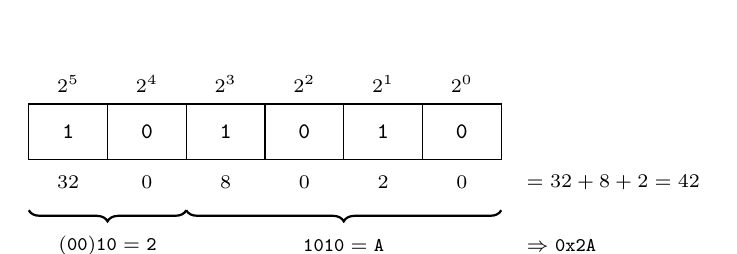
\begin{tikzpicture}[font=\footnotesize]
    \foreach \b [count=\i from 0] in {1,0,1,0,1,0} {
      \pgfmathtruncatemacro{\w}{5-\i}
      \pgfmathtruncatemacro{\val}{\b*(2^(5-\i))}
      \draw (\i,0) rectangle ++(1,0.7);
      \node at (\i+0.5,0.35) {\texttt{\b}};
      \node[font=\scriptsize] at (\i+0.5,0.95) {$2^{\w}$};
      \node[font=\scriptsize] at (\i+0.5,-0.3) {\val};
    }
    \node[anchor=west,font=\scriptsize] at (6.2,-0.3) {$=32+8+2=42$};
    \draw[decorate,decoration={brace,amplitude=4pt,mirror},thick]
      (0,-0.65) -- (2,-0.65);
    \draw[decorate,decoration={brace,amplitude=4pt,mirror},thick]
      (2,-0.65) -- (6,-0.65);
    \node[font=\scriptsize] at (1,-1.1) {$\mathtt{(00)10}=\mathtt{2}$};
    \node[font=\scriptsize] at (4,-1.1) {$\mathtt{1010}=\mathtt{A}$};
    \node[anchor=west,font=\scriptsize] at (6.2,-1.1) {$\Rightarrow \mathtt{0x2A}$};
  \end{tikzpicture}
\end{figure}

Hexadecimal uses the digits $0$ to $9$ and then $\mathtt{A}\,(=10)$ to
$\mathtt{F}\,(=15)$, so that
\[
  \mathtt{0x2A} = 2\times 16^1 + 10 = 32 + 10 = 42.
\]
\begin{notation}[Prefixes]
  \texttt{0b} marks une représentation binaire and \texttt{0x} celle
  hexadécimale. C uses these same prefixes.
\end{notation}

\subsubsection{Endianness (petit-boutien / grand-boutien)}
\begin{definition}[Grand-boutien (\textit{big-endian}) and petit-boutien (\textit{little-endian})]
  In \textbf{grand-boutien} order the octets are written classically with the
  most significant octet first. In \textbf{petit-boutien} order, often when the
  size of the words is known, the least significant octet comes first: if $m =
  o_1 o_2$ then
  \[
    m = o_1 + 256\, o_2 .
  \]
\end{definition}
\begin{figure}[h!]
  \centering
  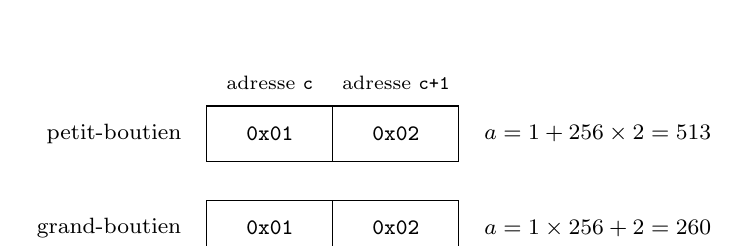
\begin{tikzpicture}[font=\footnotesize]
    % little endian
    \node[anchor=east] at (-0.2,1.35) {petit-boutien};
    \draw (0,1) rectangle ++(1.6,0.7); \node at (0.8,1.35) {\texttt{0x01}};
    \draw (1.6,1) rectangle ++(1.6,0.7); \node at (2.4,1.35) {\texttt{0x02}};
    \node[anchor=west] at (3.4,1.35)
      {$a = 1 + 256\times 2 = 513$};
    % big endian
    \node[anchor=east] at (-0.2,0.15) {grand-boutien};
    \draw (0,-0.2) rectangle ++(1.6,0.7); \node at (0.8,0.15) {\texttt{0x01}};
    \draw (1.6,-0.2) rectangle ++(1.6,0.7); \node at (2.4,0.15) {\texttt{0x02}};
    \node[anchor=west] at (3.4,0.15)
      {$a = 1\times 256 + 2 = 260$};
    % addresses
    \node[font=\scriptsize] at (0.8,2.0) {adresse \texttt{c}};
    \node[font=\scriptsize] at (2.4,2.0) {adresse \texttt{c+1}};
  \end{tikzpicture}
\end{figure}
\begin{remark}
  x86-64 is petit-boutien and is used hereinafter.
\end{remark}

\subsection{Complément à Deux}
Negative integers are represented in \textbf{complement à deux} (\textit{two's
complement}) on $k$ bits.\\

Mathematically, this allows the numbers to live in $\zee/2^{k}\zee$. The
operations $+$, $-$ and $\times$ then work regardless of whether the operands
are positive or negative. This does \emph{not} extend to comparisons and to
division.

\begin{definition}[Complement à Deux]
  The bit string $b_0 \ldots b_k$ represents
  \[
    -2^{k} b_{k} + \sum_{i<k} b_i 2^{i}.
  \]
  The most significant bit is a sign bit: $-1$ is written
  $\mathtt{0xFFFF}\ldots$, and the sign bit is used to invert the comparisons.
\end{definition}

\begin{figure}[h!]
  \centering
  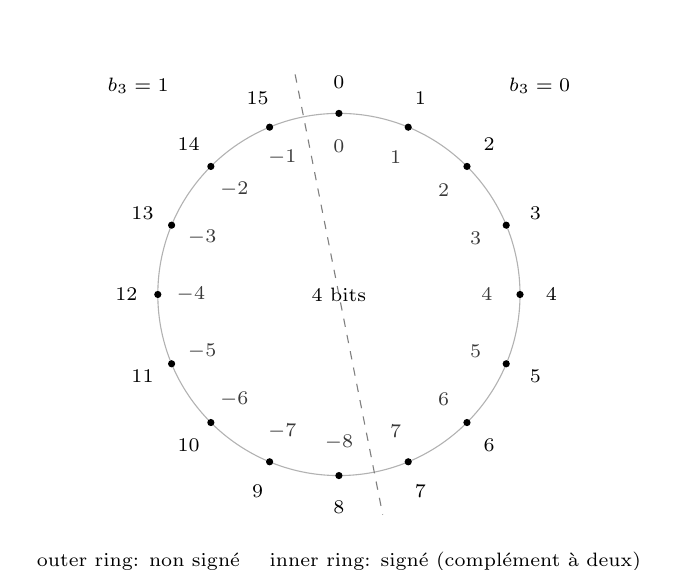
\begin{tikzpicture}[font=\scriptsize]
    \def\R{2.3}
    \draw[gray!60] (0,0) circle (\R);
    \draw[dashed,gray] (101.25:\R+0.55) -- (-78.75:\R+0.55);
    \foreach \u in {0,...,15} {
      \pgfmathsetmacro{\ang}{90 - \u*22.5}
      \pgfmathtruncatemacro{\s}{\u<8 ? \u : \u-16}
      \fill (\ang:\R) circle (1.3pt);
      \node at (\ang:\R+0.40) {\u};
      \node[gray!45!black] at (\ang:\R-0.42) {$\s$};
    }
    \node[font=\scriptsize,align=center] at (0,0) {4 bits};
    \node[font=\scriptsize] at (-2.55,\R+0.35) {$b_3=1$};
    \node[font=\scriptsize] at (2.55,\R+0.35) {$b_3=0$};
    \node[font=\scriptsize,anchor=north] at (0,-\R-0.85)
      {outer ring: non signé \quad inner ring: signé (complément à deux)};
  \end{tikzpicture}
\end{figure}

\begin{example}[Eight bits]
  $\mathtt{0x00}=0$, $\mathtt{0x7F}=127$, $\mathtt{0x80}=-128$,
  $\mathtt{0xFF}=-1$. The last follows from the formula: all bits set gives
  $-2^7 + (2^7-1) = -1$.
\end{example}

\subsection{Code ASCII}
ASCII is a table of characters on $7$ bits, i.e.\ the range $[0-127]$. It
covers the basic US characters and a set of ``control'' characters.
\begin{center}
  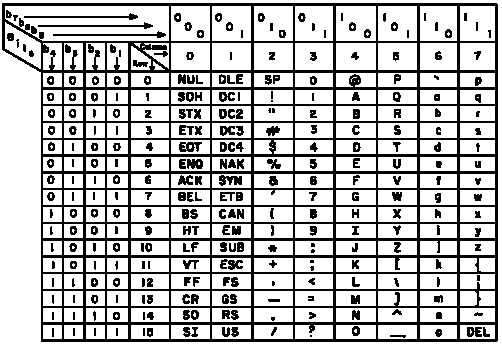
\includegraphics[width=0.75\textwidth]{ascii-table.pdf}
\end{center}

\subsection{Unités de Mémoire}
The definitions used in these notes for memory units are those of the C
standard, which are also those of the x86-64 architecture. The table below
gives the size of each unit and the number of values it can represent.
\begin{center}
  \begin{tabular}{lcc}
    \toprule
    & taille & \#~valeurs \\
    \midrule
    bit         & ---       & $2$ \\
    octet/byte  & 8 bits    & $256$ \\
    mot/word    & 2 octets  & $65\,536$ \\
    double      & 4 octets  & $\sim 4\cdot 10^{9}$ \\
    quad        & 8 octets  & $\sim 18\cdot 10^{18}$ \\
    \bottomrule
  \end{tabular}
  \hspace{1.2cm}
  \begin{tabular}{lcc}
    \toprule
    Type C & mini & courant \\
    \midrule
    \texttt{char}      & 8  & 8  \\
    \texttt{short}     & 16 & 16 \\
    \texttt{int}       & 16 & 32 \\
    \texttt{long}      & 32 & 64 \\
    \texttt{long long} & 64 & 64 \\
    \bottomrule
  \end{tabular}
\end{center}

\begin{remark}
  \textit{mot} désigne parfois le nombre de bits du processeurs (64 sur les
  processeurs modernes).
\end{remark}

The table on the right gives, for each C type, the width the standard
\emph{guarantees} and the width used in common implementations.

\subsection{Rappels de C}
C'est un langage de programmation qui est \textbf{proche de la machine}
(\textit{low-level}), \textbf{impératif}, avec \textbf{passage par valeur}
(\textit{pass-by-value}), \textbf{statiquement typé}, et l'indentation ne joue
aucun rôle (contrairement à Python).

\section{Compilateurs}
A compilateur (\textit{compiler}) are software systems that translates from
the programming languages that humans write into a form in which it can be executed
by a computer. 

\begin{definition}[Compilateur]
  Un \textbf{compilateur} est un programme qui traduit un ``programme'' d'un
  langage à un autre en préservant la sémantique.
\end{definition}
\begin{example}[Compilateurs]
  ocamlopt, latex, gcc
\end{example}

An interpréteur is another common kind of language processor, which reads a
program and executes it directly, without producing a separate output file. The
machine-language target program produced by a compilateur is typically much
faster, but an interpréteur often gives better error diagnostics.\\

\begin{example}[Hybrid systems]
  Certain language processors systems, such as Java's \texttt{javac} and
  \texttt{java}, combine both approaches: \texttt{javac} compiles Java source
  into an intermediate bytecode, which \texttt{java} then interprets.
\end{example}

\paragraph{Properties of a compilateur}:
\begin{itemize}
  \item Correct: le code compilé fait ce que l'on attend;
  \item Fast: le compilateur compile rapidement; and
  \item Optimising: le compilateur produit un code efficace.
\end{itemize}

\subsection{Grandes étapes de compilation}
This mapping between the source program to the target program is done in two main parts:
\textbf{analysis} and \textbf{synthesis}.

\begin{figure}[h!]
  \centering
  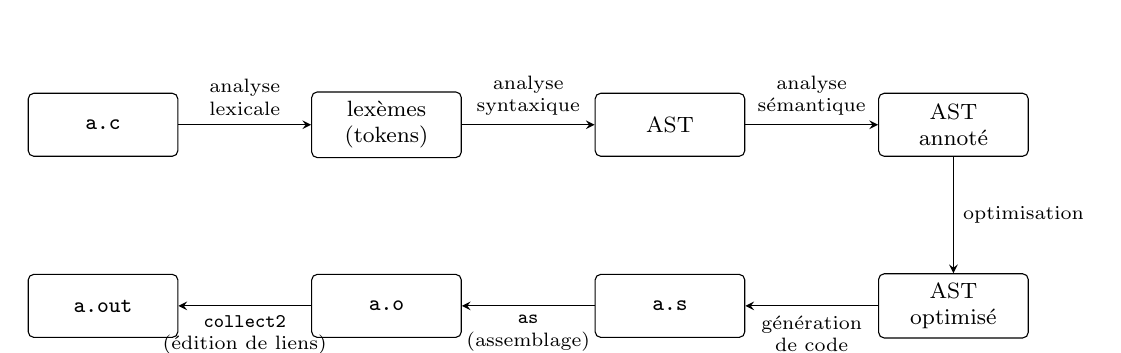
\begin{tikzpicture}[
      font=\footnotesize, >=stealth,
      box/.style={draw, rounded corners=2pt, minimum height=8mm,
                  minimum width=19mm, align=center},
      lab/.style={font=\scriptsize, align=center}
    ]
    \node[box] (c)   at (0,0)     {\texttt{a.c}};
    \node[box] (tok) at (3.6,0)   {lexèmes\\(tokens)};
    \node[box] (ast) at (7.2,0)   {AST};
    \node[box] (sem) at (10.8,0)  {AST\\annoté};
    \node[box] (opt) at (10.8,-2.3) {AST\\optimisé};
    \node[box] (asm) at (7.2,-2.3)  {\texttt{a.s}};
    \node[box] (obj) at (3.6,-2.3)  {\texttt{a.o}};
    \node[box] (bin) at (0,-2.3)    {\texttt{a.out}};
    \draw[->] (c)   -- node[lab,above]{analyse\\lexicale} (tok);
    \draw[->] (tok) -- node[lab,above]{analyse\\syntaxique} (ast);
    \draw[->] (ast) -- node[lab,above]{analyse\\sémantique} (sem);
    \draw[->] (sem) -- node[lab,right]{optimisation} (opt);
    \draw[->] (opt) -- node[lab,below]{génération\\de code} (asm);
    \draw[->] (asm) -- node[lab,below]{\texttt{as}\\(assemblage)} (obj);
    \draw[->] (obj) -- node[lab,below]{\texttt{collect2}\\(édition de liens)} (bin);
  \end{tikzpicture}
\end{figure}

The \textit{analysis} stages breaks up the source program into constituent
peices and imposes a grammatical structure on them. It then uses this structure
to create an intermediate representation of the source program. The
\textit{synthesis} stages construct the target program from the intermediate
representation and the information in the symbol table.

\subsection{Les étapes de l'analyse}
\subsubsection{Analyse Lexicale}
\begin{definition}[Analyse lexicale (\textit{lexing})]
  L'\textbf{analyse lexicale} a pour objectif de découper le fichier en une liste de
  lexèmes (\textit{tokens}); souvent à l'aide d'expressions régulières.
\end{definition}

The lexeur is the only stage that sees the file as a sequence of characters.
After it, whitespace, indentation and line breaks no longer exist.

\begin{example}[The token stream of \texttt{fibo}]
  The source on the left lexes to the stream on the right.
  \begin{multicols}{2}
    \begin{lstlisting}[language=C]
    int fibo(int n)
    {
      if(n<=1)
        return 1;
      return
         fibo(n-1)
       + fibo(n-2);
    }
    \end{lstlisting}
    \vfill\null
    \begin{lstlisting}
    INT ID("fibo") LPAR INT ID("n") RPAR
    LBRACKET
       IF LPAR ID("n") LEQ CST(1) RPAR
         RETURN CST(1) SEMICOL
       RETURN
        ID("fibo") LPAR ID("n") MINUS CST(1) RPAR
       PLUS
        ID("fibo") LPAR ID("n") MINUS CST(2) RPAR
       SEMICOL
    RBRACKET
    \end{lstlisting}
  \end{multicols}
\end{example}

\begin{remark}
This mapping into the token stream depends on the implementation and the
grammar of the source langauge, but each token usually carries an identifier
and a value.
\end{remark}

\subsubsection{Analyse Syntaxique}
\begin{definition}[Analyse syntaxique (\textit{parsing})]
  L'\textbf{analyse syntaxique} a pour objectif de récupérer la structure du
  code, généralement sous la forme d'un \textbf{arbre de syntaxe abstrait}
  (\textit{Abstract Syntax Tree}, AST) et souvent à l'aide d'une \textbf{grammaire}.
\end{definition}

\begin{example}[The AST of \texttt{fibo}]
  The token stream on the left parses to the AST on the right.
  \begin{multicols}{2}
    \begin{lstlisting}
    INT ID("fibo") LPAR INT ID("n") RPAR
    LBRACKET
       IF LPAR ID("n") LEQ CST(1) RPAR
         RETURN CST(1) SEMICOL
       RETURN
        ID("fibo") LPAR ID("n") MINUS CST(1) RPAR
       PLUS
        ID("fibo") LPAR ID("n") MINUS CST(2) RPAR
       SEMICOL
    RBRACKET
    \end{lstlisting}
    \vfill\null
    \begin{lstlisting}[language=Caml]
    Function( "fibo", [("n",Tint)],
       Sequence(
         If(Less(Var "n", Cst 1),
            Return (Cst 1)),
         Return Plus(
           Call("fibo",[Minus(Var "n", Cst 1)]),
           Call("fibo",[Minus(Var "n", Cst 2)])
          )
       )
    )
    \end{lstlisting}
  \end{multicols}
\end{example}
\begin{remark}
  The AST is only a common form of intermediate representation used by
  compilers. Alternatives include the \textit{three-address code} and the
  \textit{control-flow graph}.
\end{remark}

\subsubsection{Analyse Sémantique}
\begin{definition}[Analyse sémantique (\textit{semantic analysis})]
  L'\textbf{analyse sémantique} checks for semantic consistency with the
  language definition, and further gathers type information and saves it.
\end{definition}
This stage does not change the shape of the tree, only annotating it and
reject semantically inconsistent programs.
\begin{remark}
  Certain language specifications may permit type conversions known as
  \textit{coercions}, which typically overloads various operators and
  functions, and require conversion between types.
\end{remark}

\subsubsection{Optimisation}
\begin{definition}[Optimisation]
  L'\textbf{optimisation} a pour objectif de produire un code plus performant.
\end{definition}
An optimisation is a rewriting of the program which must preserve the
semantics; the analyses that justify the rewriting are what the names below
refer to.

\begin{example}[Élimination du code mort (\textit{dead code elimination})]
  The call under a condition that is statically false is removed.
\begin{lstlisting}[language=C]
int fibo(int n) {                         int fibo(int n) {
  if(n<=1)                                  if(n<=1)
    return 1;                                 return 1;
  if(false)                   ==>           return
    printf("fib %d\n",n);                     fibo(n-1)
  return                                    + fibo(n-2);
     fibo(n-1)                            }
   + fibo(n-2);
}
\end{lstlisting}
\end{example}

\begin{example}[Propagation des constantes (\textit{constant propagation})]
  A product of four \texttt{const int}s is evaluated at compile time.
\begin{lstlisting}[language=C]
const int days_in_year = 365 ;                const int days_in_year = 365 ;
const int hours_in_day = 24 ;                 const int hours_in_day = 24 ;
const int min_in_hours = 60 ;         ==>     const int min_in_hours = 60 ;
const int seconds_in_hours = 60 ;             const int seconds_in_hours = 60 ;
int main() {                                  int main() {
  printf("There are %d "                        printf("There are %d "
  "seconds in an ordinary year!",               "seconds in an ordinary year!",
  days_in_year * hours_in_day *                 31536000);
  min_in_hours * seconds_in_hours );          }
}
\end{lstlisting}
\end{example}

\begin{example}[Analyse des alias (\textit{alias analysis})]
  The load is replaced by the value that was just stored.
\begin{lstlisting}[language=C]
int f(int * a, int * b) {            int f(int * a, int * b) {
  *a = 42;                             *a = 42;
  *b = 12;                  ==>        *b = 12;
  return *a;                           return 42;
}                                    }
\end{lstlisting}
  This rewrite is legal exactly when the compiler can prove that \texttt{a} and \texttt{b} do not
\emph{alias}, i.e.\ do not point at the same cell.
\end{example}

Optimisation is non-trivial, often requiring global analyses of the program,
and is a major part of the work of a compiler. There are also other forms of
optimisations, such as dépliement de boucles (\textit{loop unrolling}), analyse
de vie (\textit{liveness analysis}), dead store, and sous-expressions communes
(\textit{common subexpression elimination}).

\subsection{Les étapes de la synthèse}
\subsubsection{Code Génération}
The first stage of \textit{synthesis} is code generation, which turns the intermediate
representation into the target language. In the context of \textit{code assembleur (x86)},
this produces a (still) human-readable text file of assembly instructions.

\begin{example}[\texttt{fibo} in x86-64 AT\&T assembly]
  What \texttt{cc1} emits for the source above.
\begin{lstlisting}[language=gas]
    .file    "a.c"
    .text
    .globl   fibo
    .type    fibo, @function
fibo:
.LFB0:
    .cfi_startproc
    pushq    %rbp
    .cfi_def_cfa_offset 16
    .cfi_offset 6, -16
    movq     %rsp, %rbp
    .cfi_def_cfa_register 6
    pushq    %rbx
    subq     $24, %rsp
    .cfi_offset 3, -24
\end{lstlisting}
$\qquad\quad\vdots$
\end{example}

\begin{remark}
  The lines beginning with a dot are \textbf{directives} addressed to the
  assembler, not instructions: \texttt{.text}, \texttt{.section .rodata},
  \texttt{.globl}, \texttt{.type} and \texttt{.size} organise the output. They
  produce no machine code.
\end{remark}

\subsubsection{Assemblage}
\begin{definition}[Assemblage]
  In the context of Linux / ELF, the assembleur turns that text into an fichier
  objet (\textit{object file}). The instructions are now octets, grouped into
  named sections.
\end{definition}

\begin{example}[A hex dump of \texttt{b.o}]
  What \texttt{as} emits, section by section.
\begin{lstlisting}
b.o:     file format elf64-x86-64

Contents of section .text:
 0000 554889e5 534883ec 18897dec 837dec01  UH..SH....}...}.
 0010 7f07b801 000000eb 1e8b45ec 83e80189  ..........E.....
 0020 c7e80000 000089c3 8b45ec83 e80289c7  .........E......
 0030 e8000000 0001d848 8b5df8c9 c3        .......H.].....
Contents of section .comment:
 0000 00474343 3a202844 65626961 6e203132  .GCC: (Debian 12
 0010 2e322e30 2d31342b 64656231 32753129  .2.0-14+deb12u1)
 0020 2031322e 322e3000                     12.2.0.
Contents of section .eh_frame:
 0000 14000000 00000000 017a5200 01781001  .........zR...x.
 0010 1b0c0708 90010000 1c000000 1c000000  ................
 0020 00000000 3d000000 00410e10 8602430d  ....=....A....C.
 0030 06458303 730c0708                    .E..s...
\end{lstlisting}
\end{example}

\subsubsection{Édition de liens}
\begin{definition}[Édition de liens (\textit{linking})]
  In Linux / ELF, the linker takes one or more object files and produces a
  single executable file. It resolves the references between the object files,
  and adds the C runtime startup code and the dynamic-linking machinery.
\end{definition}
This produce the fichier binaire (\textit{binary file}) that the operating
system can load and run.

\begin{example}[A word dump inside \texttt{a.out}]
  A window onto the symbol names the linker had to resolve.
\begin{lstlisting}
0000470 5f00 6c5f 6269 5f63 7473 7261 5f74 616d
0000480 6e69 5f00 635f 6178 665f 6e69 6c61 7a69
0000490 0065 7270 6e69 6674 6c00 6269 2e63 6f73
00004a0 362e 4700 494c 4342 325f 322e 352e 4700
00004b0 494c 4342 325f 332e 0034 495f 4d54 645f
00004c0 7265 6765 7369 6574 5472 434d 6f6c 656e
00004d0 6154 6c62 0065 5f5f 6d67 6e6f 735f 6174
00004e0 7472 5f5f 5f00 5449 5f4d 6572 6769 7374
00004f0 7265 4d54 6c43 6e6f 5465 6261 656c 0000
\end{lstlisting}
Each group is a 16-bit word printed in hexadecimal. On a petit-boutien machine,
we may recover the null-terminated strings by swapping each pair of two octets
and reading the result as ASCII:
\begin{lstlisting}
__libc_start_main   __cxa_finalize   printf   libc.so.6
GLIBC_2.2.5   GLIBC_2.34   _ITM_deregisterTMCloneTable
__gmon_start__   _ITM_registerTMCloneTable
\end{lstlisting}
\end{example}

\subsection{Le Pipeline de Compilation}
\begin{example}[Linux / ELF]
  Invoking \texttt{gcc a.c} triggers three tools in sequence:
  \begin{itemize}
    \item \verb|cc1 a.c a.s| --- produce the assembly from the C;
    \item \verb|as -o a.o a.s| --- produce the object from the assembly;
    \item \verb|collect2 a.o a.out| --- produce the binary from the object.
  \end{itemize}
  Each of these tools performs its own lexical, syntactic and semantic
  analyses. Additionally, each of the intermediate files can be inspected with
  the following commands:
  \begin{itemize}
    \item \texttt{gcc -S a.c} --- produce the assembly from the C;
    \item \texttt{as -o a.o a.s} --- produce the object from the assembly;
    \item \texttt{objdump -d a.o} --- produce a disassembly of the object;
    \item \texttt{objdump -d a.out} --- produce a disassembly of the binary.
  \end{itemize}
\end{example}

The compiler is a chain of programs, each potentially taken as compilers in
their own right, with its own input and output language.

\section{Bases de x86-64}
A compiler ultimately has to emit machine code, so the bottom of the pipeline
has to be understood before the top of it means anything. This chapter is the
target language: the x86-64 \textbf{instruction set architecture}
(\textit{Instruction Set Architecture}, ISA), the GAS syntax in which it is
written by hand, and enough of Linux's system-call interface to get a program
to produce visible output without any library at all.

\subsection{Modèle Simplifié}
\subsubsection{Le Mémoire d'un Ordinateur}
Le modèle d'un ordinateur used in this course has two kinds of storage:
\textbf{Registres} (\textit{registers}), and \textbf{RAM} (\textit{Random Access Memory}). 

\begin{figure}[h!]
  \centering
  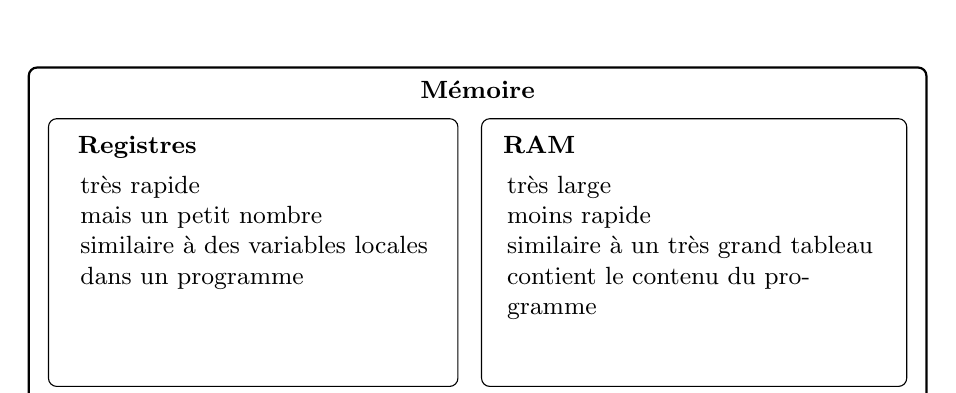
\begin{tikzpicture}[font=\small]
    \draw[rounded corners=3pt, thick] (-0.25,-0.25) rectangle (11.15,4);
    \node[anchor=north] at (5.45,3.95) {\textbf{Mémoire}};
    \draw[rounded corners=3pt] (0,-0.05) rectangle (5.2,3.35);
    \node[anchor=north west] at (0.25,3.25) {\textbf{Registres}};
    \node[anchor=north west, text width=4.55cm] at (0.28,2.75)
      {très rapide\\ mais un petit nombre\\ similaire à des variables locales dans un programme};
    \draw[rounded corners=3pt] (5.5,-0.05) rectangle (10.9,3.35);
    \node[anchor=north west] at (5.65,3.25) {\textbf{RAM}};
    \node[anchor=north west, text width=4.7cm] at (5.7,2.75)
      {très large\\ moins rapide\\ similaire à un très grand tableau\\ contient le contenu du programme};
  \end{tikzpicture}
\end{figure}

\subsubsection{Le Programme}
\begin{definition}[Programme]
  Un \textbf{programme} ce sont des instructions dans la RAM à une adresse.
\end{definition}
Un registre spécial --- \verb|%rip| en x86-64, le \textbf{pointeur d'instruction}
(\textit{instruction pointer}) --- contient l'adresse de l'instruction courante.\\

Chaque instruction peut:
\begin{itemize}
  \item lire ou écrire des registres;
  \item lire ou écrire une case de la RAM; ou
  \item faire un appel à l'OS (\textbf{syscall}).
\end{itemize}

\begin{remark}
  Ce modèle ne gère pas : disque, écran, clavier, souris, etc. Tous les effets
  du programme sur le monde extérieur passent par l'OS.
\end{remark}

\begin{example}[Factorial of $R_0$ in the abstract model]
  With registers $R_0$, $R_1$ and $R_{IP}$, the factorial of $R_0$ is computed
  by the following six instructions. Only the writes to $R_{IP}$ make control
  flow.

  \medskip
  \centering
  \begin{tabular}{c l l}
    \toprule
    Instruction & Effect & \\
    \midrule
    0 & $R_1 = 1$, \quad $R_{IP} = R_{IP} + 1$ & $R_{IP}$ = next instruction \\
    1 & if $R_0 = 0$ then $R_{IP} = 5$, else $R_{IP} = R_{IP} + 1$ & conditional jump \\
    2 & $R_1 = R_0 \times R_1$, \quad $R_{IP} = R_{IP} + 1$ & \\
    3 & $R_0 = R_0 - 1$, \quad $R_{IP} = R_{IP} + 1$ & \\
    4 & $R_{IP} = 1$ & unconditional jump \\
    5 & rest of the program, or end & \\
    \bottomrule
  \end{tabular}
\end{example}

\subsection{L'Assembleur}
\begin{definition}[Assembleur]
  \textbf{Assembleur} est le langage lisible dans lequel on écrit du code
  traduit ensuite vers du binaire. Aussi: Le programme qui fait cette traduction.
\end{definition}
\subsubsection{Instruction Set Architecture}
\begin{definition}[Instruction Set Architecture (ISA)]
  \textbf{ISA} est l'ensemble des instructions qu'un processeur peut exécuter,
  et la manière dont elles sont codées en binaire.
\end{definition}

The assembleur depends on the ISA but there may be multiple syntaxes for
the same ISA.
\begin{example}[Intel vs AT\&T/GAS syntax]
  The Intel syntax is used in the Intel manuals and in the Visual Studio IDE.
  The AT\&T/GAS syntax is used by the GNU Assembler (GAS) and by GCC.
  Between the two syntaxes the order of operands is reversed: Intel writes
  \verb|mov rax, rbx| while GAS writes \verb|mov %rbx, %rax|.
\end{example}

\subsubsection{Le Format Binaire}
\begin{definition}[Processus]
  Un \textbf{processus} (\textit{process}) est un programme en cours d'exécution. Il peut
  aussi être vu comme un état de la mémoire: le contenu des registres et de la RAM.
\end{definition}
\begin{definition}[Exécutable]
  Un \textbf{exécutable} (\textit{executable}) est un fichier qui contient un
  programme et les informations nécessaires pour que l'OS le charge en mémoire
  et lancer le processus correspondant.
\end{definition}
There are several formats for exécutables:
\begin{itemize}
  \item \textbf{Executable and Linking Format} (ELF) under Unix, except Mac;
  \item \textbf{Portable Executable} under Windows;
  \item \textbf{Mach-O} or PEF under Mac.
\end{itemize}

\begin{remark}
  In this course, we study the ELF format, used in Linux, with the x86-64 ISA
  and the GAS syntax.
\end{remark}

\subsection{La mémoire en x86-64}
\subsubsection{Les Registres Généraux}
x86-64 exposes sixteen 64-bit registres généraux:
\begin{center}
  \begin{tabular}{l l @{\qquad\qquad} l l}
    \toprule
    \multicolumn{2}{c}{Compute registers} & \multicolumn{2}{c}{Pointer registers} \\
    Name & ``Historical'' function & Name & ``Historical'' function \\
    \midrule
    \verb|rax| & Accumulator & \verb|rsi| & Source index \\
    \verb|rbx| & Base        & \verb|rdi| & Destination index \\
    \verb|rcx| & Counter     & \verb|rsp| & Stack Pointer \\
    \verb|rdx| & Data        & \verb|rbp| & Base Pointer \\
    \bottomrule
  \end{tabular}
\end{center}

\noindent along with 8 x86-64 registers with no pre-established function,
\verb|r8| through \verb|r15|.

Each register can be addressed at four widths by their \textbf{sous-registres}
(\textit{subregisters}), each a \emph{part of} the same physical register. e.g.
Writing \verb|%al| leaves the upper 56 bits of \verb|%rax| untouched.

\begin{center}
  \begin{tabular}{l l l l l}
    \toprule
    $b_0 \dots b_{63}$ & $b_0 \dots b_{31}$ & $b_0 \dots b_{15}$ & $b_8 \dots b_{15}$ & $b_0 \dots b_7$ \\
    Quad (q) & Double (d/l) & Word (w) & Byte (b) & Byte \\
    \midrule
    \verb|rax| & \verb|eax| & \verb|ax| & \verb|ah| & \verb|al| \\
    \verb|rbx| & \verb|ebx| & \verb|bx| & \verb|bh| & \verb|bl| \\
    \verb|rcx| & \verb|ecx| & \verb|cx| & \verb|ch| & \verb|cl| \\
    \verb|rdx| & \verb|edx| & \verb|dx| & \verb|dh| & \verb|dl| \\
    \verb|rsi| & \verb|esi| & \verb|si| &            & \verb|sil| \\
    \verb|rdi| & \verb|edi| & \verb|di| &            & \verb|dil| \\
    \verb|rsp| & \verb|esp| & \verb|sp| &            & \verb|spl| \\
    \verb|rbp| & \verb|ebp| & \verb|bp| &            & \verb|bpl| \\
    \verb|r8|  & \verb|r8d| & \verb|r8w| &           & \verb|r8b| \\
    \bottomrule
  \end{tabular}
\end{center}

The \verb|r8| row is the pattern for all eight registers:
\verb|r|$n$\verb|d|, \verb|r|$n$\verb|w|, \verb|r|$n$\verb|b|.

\begin{remark}
  The suffix letters \verb|q|, \verb|l|, \verb|w|, \verb|b| can also be
  appended to instructions to state how many bytes the operation touches.
\end{remark}

\subsubsection{Adressage Virtuel}
Memory is seen as an array of $2^{64}$ bytes. Each process has its own
translation from the address to memory, which is not necessarily on the RAM.
This translation is provided by the OS, depending on its state of paging.
\begin{figure}[h!]
  \centering
  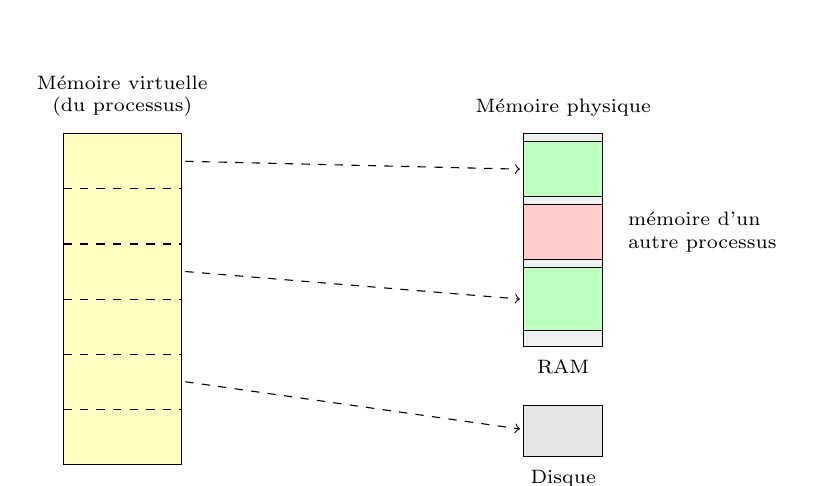
\begin{tikzpicture}[font=\small]
    \node[anchor=south, align=center, font=\scriptsize] at (1,4.3)
      {Mémoire virtuelle\\ (du processus)};
    \draw[fill=yellow!25] (0.25,0) rectangle (1.75,4.2);
    \foreach \y in {0.7,1.4,2.1,2.8,3.5} { \draw[dashed] (0.25,\y) -- (1.75,\y); }

    \node[anchor=south, align=center, font=\scriptsize] at (6.6,4.3) {Mémoire physique};
    \draw[fill=gray!12] (6.1,1.5) rectangle (7.1,4.2);
    \draw[fill=green!25] (6.1,3.4) rectangle (7.1,4.1);
    \draw[fill=red!20]   (6.1,2.6) rectangle (7.1,3.3);
    \draw[fill=green!25] (6.1,1.7) rectangle (7.1,2.5);
    \node[anchor=west, font=\scriptsize, align=left] at (7.3,2.95)
      {mémoire d'un\\ autre processus};
    \node[anchor=north, font=\scriptsize] at (6.6,1.45) {RAM};

    \draw[fill=gray!20] (6.1,0.1) rectangle (7.1,0.75);
    \node[anchor=north, font=\scriptsize] at (6.6,0.05) {Disque};

    \draw[->, dashed] (1.8,3.85) -- (6.05,3.75);
    \draw[->, dashed] (1.8,2.45) -- (6.05,2.1);
    \draw[->, dashed] (1.8,1.05) -- (6.05,0.45);
  \end{tikzpicture}
\end{figure}

\subsection{Programmation en GAS}
\paragraph{Définir des sections en GAS} Based on the mémoire virtuelle of the
processus, we may hence define the sections in which our data lives:
\begin{lstlisting}[language=gas]
        .text # debut d'une section de code
# ce qui est defini ici (donnees ou instructions) est executable

        .data # section de donnees modifiables
# ce qui est defini ici est modifiable mais n'est pas executable
.quad 0x1234567890 # la section commence par
      # 8 octets contenant le nombre 0x1234567890
      # qui prend minimum 5 octets a etre stocke
.byte 0x12 ; ces 8 octets sont suivi par un octet contenant
      ; 0x12 (=18 en decimal)
.ascii "Hello " ; H, e, l, l, o, ' '
.asciz "World" ; 6 octets W, o, r, l, d, \0
.helloworld: ; un label, une maniere d'adresser
        .string        "Hello World!\n" # la meme chose que asciz, donc 13+1=14 octets

        .bss # section de donnees modifiables initialisees a 0

        .text         # une autre section de code
        .globl _start # on veut exporter ce symbole
_start: # le label main correspondra a une function
        movq $42, .x(%rip)
        ret

# GCC rale si on ne finit pas par une speciale section protegee
.section        .note.GNU-stack,"",@progbits
\end{lstlisting}

\begin{remark}
  The trailing \verb|.note.GNU-stack| is required for the linker in \verb|gcc|
  to be able to certify that the program does not want an executable pile.
\end{remark}

\subsubsection{Registres et constantes, accès à la RAM}
In GAS,
\begin{itemize}
  \item on préfixe les registres par \verb|%| --- \verb|%rip|, \verb|%rbx|, etc.;
  \item on préfixe les nombres par \verb|$| --- \verb|$42|, \verb|$0x2A|, etc.
\end{itemize}
Plus généralement, \verb|offset(base, index, scale)| accède à
\[
  \text{offset} + v(\text{base}) + v(\text{index}) \times \text{scale},
\]
avec \textit{offset} en constante 32 bits signés, \textit{base} un registre,
\textit{index} un registre, \textit{scale} un entier parmi
$1, 2, 4, 8$. Any of the four parts may be omitted. On peut lire ou écrire
$1$, $2$, $4$ ou $8$ octets consécutifs.

\begin{center}
  \begin{tabular}{l l}
    \toprule
    Operand & Cell addressed \\
    \midrule
    \verb|(%rsp)|            & la case à la valeur de \verb|%rsp| \\
    \verb|4(%rsp)|           & la case à la valeur de $4 + $ \verb|%rsp| \\
    \verb|4(%rsp,%rdi,2)|    & la case à la valeur de $4 + $ \verb|%rsp| $+\, 2 \times$ \verb|%rdi| \\
    \verb|x(%rip)|           & the cell at the label \verb|x| (see below) \\
    \bottomrule
  \end{tabular}
\end{center}

\paragraph{Labels et multisections} Un registre spécial (\text{\%rip} en
x86-64) stocke l'adresse de l'instruction courante. Labels store
addresses relative to \text{\%rip}, so that the code can be
position-independent. We may hence use labels to obtain the address of a stored
variable:

\begin{lstlisting}[language=gas]
        .text
.globl _start # marque que le symbole _start sera visible
_start:       # dans le fichier ELF produit
      # differents adressages
      mov x(%rip), %rax # relatif
      lea x(%rip), %rcx # adresse
      ### toujours mettre label(%rip) pour parler de la valeur
      # a la position du label
# on n'est pas oblige de changer de section
# pour stocker notre nombre
x: .quad 0x1234567890
\end{lstlisting}

\begin{example}[Copying Data]
La copie de données se fait avec \verb|mov source destination| où \verb|source| et
\verb|destination| peuvent être :
\begin{itemize}
  \item un nombre comme \verb|$42| (décimal) ou \verb|0x2A| en hexadécimal;
  \item un registre \verb|%rbx|;
  \item une case mémoire \verb|(%rsp)|, \verb|4(%rsp)|, \verb|18(%rsp,%rax,4)|,
    \verb|x(%rip)|.
\end{itemize}
\begin{remark}
On peut spécifier le nombre d'octets à copier. It is specified with the suffixes
\verb|b|, \verb|w|, \verb|l| and \verb|q| for $1$, $2$, $4$ and $8$ bytes,
respectively. L'assembleur tente de deviner le nombre d'octets à copier mais ce
n'est pas toujours possible, p.~ex.\ \verb|mov $42, (%rsp)|. When the suffix is
omitted the guess is made from the operands, and there it fails because neither
operand carries a width. Toutes les combinaisons source/destination ne sont pas
possibles. Memory to memory copies, for instance, are not allowed, so
\verb|mov (%rsp),(%rax)| is illegal.
\end{remark}
\end{example}

\begin{lstlisting}[language=gas]
mov $42, %rax
mov helloworld(%rip), %rsi
mov $42, %eax
mov $42, %ax
mov $42, %al
movb $0x12, (%rax) ; ecrit un seul octet (byte)
movw $0x1234, (%rax) ; ecrit un mot (2 O)
movl $0x12345678, (%rax) ; ecrit mot long (4 O)
movq $0x12345678, (%rax) ; ecrit un quad (8 O)
                         ; en utilisant un 32 bits signe
movq $0x4883ec08, 4(%rip)
\end{lstlisting}

\subsubsection{Casting}
Extending a value from a smaller width to a larger one is called
\textbf{casting}. In x86-64, the choice between the two forms is the choice of
how the new high bits are filled.

\begin{example}[Casting]
  \verb|movq $0x12345678, (%rax)| writes \verb|0x0000000012345678|, while
  \verb|movq $0xFFFFFFFF, (%rax)| writes \verb|0xFFFFFFFFFFFFFFFF|, since
  the immediate is encoded as a signed 32-bit value and sign-extended to
  64 bits.
\end{example}

We may hence specify the extension from a source width to a destination width
with zero- or sign-extension:
\begin{lstlisting}[language=gas]
movzbl %al, %ecx ; extension with Zero
movswq %ax , %rcx ; extension Signed:
                  ; 1 if starts with 1, 0 otherwise
\end{lstlisting}

\begin{example}[C to Assembly]
  We then have the following example of a C program and its translation to assembly, obtained
  with \verb|gcc -S -O0|. Note that an \verb|int| is four bytes, so we use \verb|movl| and
  store it in a \verb|.long|; the \verb|pushq %rbp| / \verb|movq %rsp, %rbp| /
  \verb|popq %rbp| trio is the function prologue and epilogue; and the valeur de
  retour of \verb|main| is stored in \verb|%eax|.
  \begin{multicols}{2}
    \begin{lstlisting}[language=C]
    int x = 0x12;   // 18
    int main() {
      x = 0x34;     // 52
      x = 0x56;     // 86
      x = 0x78;     // 120
    }
    \end{lstlisting}\vfill\null
    
    \begin{lstlisting}[language=gas]
            .globl  x
            .data
    x:      .long   18
            .text
            .globl  main
    main:
            pushq   %rbp
            movq    %rsp, %rbp
            movl    $52, x(%rip)
            movl    $86, x(%rip)
            movl    $120, x(%rip)
            movl    $0, %eax
            popq    %rbp
            ret
    \end{lstlisting}
  \end{multicols}
\end{example}

\begin{example}[Disassembly]
  Below is the disassembly of the previous example. Utilisation de
  \verb|objdump -S| pour le \verb|main| et \verb|-d| pour le data.
  \begin{lstlisting}
  0000000000001129 <main>:
    1129: 55                      push %rbp
    112a: 48 89 e5                mov %rsp,%rbp
    112d: c7 05 d9 2e 00 00 34    movl $0x34,0x2ed9(%rip) # 4010 <x>
    1134: 00 00 00
    1137: c7 05 cf 2e 00 00 56    movl $0x56,0x2ecf(%rip) # 4010 <x>
    113e: 00 00 00
    1141: c7 05 c5 2e 00 00 78    movl $0x78,0x2ec5(%rip) # 4010 <x>
    1148: 00 00 00
    114b: b8 00 00 00 00          mov $0x0,%eax
    1150: 5d                      pop %rbp
    1151: c3                      ret
  .....
  Contents of section .data:
   4000 00000000 00000000 08400000 00000000 .........@......
   4010 12000000                            ....
  \end{lstlisting}
\end{example}
\begin{remark}
  Instructions are variable-length on x86-64. The three \verb|movl| stores
  each occupy ten bytes while \verb|ret| occupies one. 
\end{remark}

\subsubsection{Arithmétique}
\begin{lstlisting}[language=gas]
add $42, %rax ; %rax += 42
add $-4, %rsp ; %rsp += -4
add %rax, %rbx ; %rbx += %rax
sub %rax, %rbx ; %rbx -= %rax
inc %rbx ; %rbx++
incq (%rsp) ; interpret the 8 byte at positions %rsp
decq (%rsp) ; as an integer and inc/dec them
cmp %rax, %rbx ; compute the diff but stores nothing
\end{lstlisting}
\begin{lstlisting}[language=gas]
imul $42, %rax ; %rax *= 42
imul %rbx ; %rax = (%rax * %rbx) mod 2^64
          ; %rdx = (%rax * %rbx) / 2^64
          ; or %rax:%rdx = (%rax * %rbx)
          ; as signed 128 bits int
mul %rbx ; %rax:%rdx = %rbx * %rax unsigned

idiv %rbx ; %rax = computes %rax + 2^64 x %rdx / %rbx
          ; %rdx is the remainder % %rbx
          ; idivq segfaults if the result does not fit

lea -8(%rsp, %rdx,4), %rax ; %rax = -8+%rsp+%rdx*4
      ; usually used to compute addresses
\end{lstlisting}

The one-operand forms are implicit in \verb|%rax| and \verb|%rdx|. For division
the dividend is the 128-bit quantity \verb|%rdx:%rax|:
\[
  \texttt{\%rax} \seteq
    \myfloor{\frac{2^{64}\,\texttt{\%rdx} + \texttt{\%rax}}{\texttt{\%rbx}}},
  \qquad
  \texttt{\%rdx} \seteq
    \left(2^{64}\,\texttt{\%rdx} + \texttt{\%rax}\right) \mod \texttt{\%rbx}.
\]

\subsubsection{Manipulation Bit-À-Bit}
\begin{lstlisting}[language=gas]
not %rax ; reverse all bits
xor %rax, %rbx ; %rbx ^= %rax
or %rax, %rbx ; %rbx |= %rax
and %rax, %rbx ; %rbx &= %rax

sal $42, %rax ; Shift arithmetic left
sar $42, %rax ; Shift arithmetic right
shr $42, %rax ; Shift (logic) right

test %rax, %rbx ; computes & but stores nothing
\end{lstlisting}

\subsubsection{Sauts}
\begin{lstlisting}[language=gas]
jmp main ; go to main, do not put (%rip) here
jmp *%rax ; go to the address pointed by %rax
\end{lstlisting}

A jump target is a label written bare --- \emph{not} \verb|main(%rip)|, because
the operand of a jump already is an address rather than the contents of one.
The starred form \verb|jmp *%rax| is the indirect jump, and it is what function
pointeurs, \verb|switch| tables and virtual dispatch all compile to.

\subsubsection{Drapeaux Utiles}
Il existe un \textbf{registre de drapeaux} (\textit{flags register}) spécial, on
y retrouve les drapeaux suivants :
\begin{center}
  \begin{tabular}{c c l l}
    \toprule
    Bit & Abréviation & Nom & Description \\
    \midrule
    0  & CF & Carry Flag    & retenue ? (was there a carry?) \\
    2  & PF & Parity Flag   & pair ou impair ? (even or odd?) \\
    6  & ZF & Zero Flag     & nul ? (is it zero?) \\
    7  & SF & Sign Flag     & strictement négatif ? (strictly negative?) \\
    11 & OF & Overflow Flag & le calcul signé a débordé ? (did the signed computation overflow?) \\
    \bottomrule
  \end{tabular}
\end{center}

\subsubsection{Instructions Conditionnelles}
\begin{lstlisting}[language=gas]
jCOND fact ; jump on COND
cmovCOND %rbx, %rcx ; mov on COND
setCOND %rax ; set %rax to 1 when COND
             ; and to 0 otherwise
\end{lstlisting}

Every condition is invertible by inserting \verb|n|, so \verb|jne| is the
negation of \verb|je|, \verb|cmovnz| of \verb|cmovz|, and so on. Quelques
conditions usuelles :

\begin{center}
  \begin{tabular}{l l @{\qquad\qquad} l l}
    \toprule
    \verb|e|  & equal                     & \verb|ae| & above or equal / unsigned \\
    \verb|z|  & zero (same as above)      & \verb|g|  & greater / signed \\
    \verb|ge| & greater equal             & \verb|l|  & less / signed \\
    \verb|b|  & below / unsigned          & \verb|ge| & greater or equal / signed \\
    \verb|a|  & above / unsigned          & \verb|le| & less or equal / signed \\
    \verb|be| & below or equal / unsigned & \verb|p|  & parity is even \\
    \bottomrule
  \end{tabular}
\end{center}

\subsubsection{Interaction avec l'OS}
En x86-64, c'est la commande \verb|syscall| qui rend la main à
l'OS. The syscall number goes in \verb|%rax| and the arguments in \verb|%rdi|,
\verb|%rsi|, \verb|%rdx| (and then \verb|%r10|, \verb|%r8|, \verb|%r9|).

\begin{center}
  \begin{tabular}{c l c c c}
    \toprule
    \verb|%rax| & Nom & \verb|%rdi| & \verb|%rsi| & \verb|%rdx| \\
    \midrule
    0  & Read  & \verb|fd|    & \verb|char*| & \verb|count| \\
    1  & Write & \verb|fd|    & \verb|char*| & \verb|count| \\
    12 & Break & \verb|brk|   &              &              \\
    60 & Exit  & \verb|error| &              &              \\
    \bottomrule
  \end{tabular}
\end{center}

\begin{remark}
  En Linux tout est fichier notamment l'entrée, la sortie et la sortie d'erreur
  avec les \textbf{descripteurs de fichiers} (\textit{file descriptors},
  \verb|fd|) $0$, $1$, et $2$. On désigne par \verb|fd| $0$ la entrée standard,
  et par \verb|fd| $1$ la sortie standard.
\end{remark}

\subsection{Exercices: Programmation en GAS}

\begin{problem}[A program that does nothing]
\begin{lstlisting}[language=gas]
        .globl _start
_start:
        mov $60, %rax ; id of the syscall
        xor %rdi, %rdi ; a trick to set %rdi to 0
        syscall

        .section .note.GNU-stack ; pour gcc
\end{lstlisting}
\end{problem}

\begin{remark}
  The \verb|syscall| instruction is required to terminate the program,
  otherwise the CPU will continue executing off into whatever bytes follow.
\end{remark}

\begin{problem}[Hello World]
  Pour l'appel \verb|Write| il faut \verb|%rax| $= 1$; la chaîne a une longueur
  de $13$; et il faut un pointeur vers la chaîne dans \verb|%rsi|.  Pour avoir
  le pointeur, il faut que \verb|"Hello World!\n"| existe dans la mémoire; il
  faut trouver son adresse et la mettre dans \verb|%rsi|.
\begin{lstlisting}[language=gas]
        .data
helloWorld:
        .string "Hello World!\n"
        .text
        .globl _start
_start:
        lea helloWorld(%rip), %rsi ; load the address of the string
        mov $1, %rdi ; stdout = 1
        mov $13,%rdx ; size of string to be printed
        mov $1, %rax ; id of the syscall
        syscall
        mov $60, %rax
        xor %rdi, %rdi
        syscall
        .section .note.GNU-stack
\end{lstlisting}
\end{problem}

\begin{problem}[Hello World 10 times]
\begin{lstlisting}[language=gas]
_start:
        mov $10, %r8
.boucle:
        lea helloWorld(%rip), %rsi
        mov $1,        %rdi
        mov $13,%rdx
        mov $1, %rax
        syscall
        dec %r8
        jnz .boucle
        mov $60, %rax
        xor %rdi, %rdi
        syscall
        .section .note.GNU-stack
\end{lstlisting}
  On utilise \verb|dec| pour décrémenter et \verb|jnz| pour jump non zero. With
  these, a counter in \verb|%r8| turns the body into a loop.
\end{problem}

\begin{remark}
  Not all registres d'argument are preserved across a \verb|syscall|, and there
  is no guarantee that the kernel will not trash them, without knowing the
  implementation of the syscall.
\end{remark}

\subsubsection{Autres Exercices}
\begin{center}
  \begin{tabular}{l r}
    \toprule
    Consigne & Exemple \\
    \midrule
    afficher une ligne de \verb|'X'| & \verb|XXXXXX| \\
    afficher une pyramide de \verb|'O'| & \verb|OO| puis \verb|O| \\
    afficher une chaîne dont on ne connaît pas la longueur & \verb|Hello !| \\
    afficher un caractère stocké dans \verb|%r8| $(\dagger)$ & \verb|'c'| $= 99$ \\
    afficher en décimal petit-boutien l'entier dans \verb|%r8| & \verb|24| \\
    calculer $10!$ avec une boucle & \verb|3628800| \\
    \bottomrule
  \end{tabular}
\end{center}

% The x86-64 reference sheet: after chapter 2, on pages of its own, on the model
% of Stanford CS107's x86-64 Reference Sheet. Unnumbered, so chapters 3--6 keep
% their numbers. Content and verification:
% docs/superpowers/specs/2026-09-21-ece-3tc32-x86-reference-sheet-design.md
%
% Every tabularx whose first column is instruction or directive syntax is
% preceded by the line "% syntax-table": the verification script reads those
% rows and requires each mnemonic to have been assembled.
\clearpage
\newgeometry{hmargin=0.6in, top=0.9in, bottom=0.6in, headheight=14pt}
\setlength{\headwidth}{\textwidth}
\phantomsection
\section*{Aide-mémoire x86-64}
\addcontentsline{toc}{section}{Aide-mémoire x86-64}
\markright{\textsf{Aide-mémoire x86-64}}

\begingroup
\footnotesize
\setlength{\tabcolsep}{4pt}
\setlength{\columnsep}{18pt}
\setlength{\belowbottomsep}{3pt}          % keep a note clear of a table's \bottomrule
\renewcommand{\tabularxcolumn}[1]{>{\raggedright\arraybackslash}p{#1}}   % no stretched cells
\raggedcolumns
\raggedright                              % a reference sheet: no stretched prose lines
\microtypesetup{protrusion=false}         % keep typewriter text inside its column
\newcommand{\sheethead}[1]{%
  \par\medskip\noindent{\small\sffamily\bfseries #1}\par\nopagebreak\smallskip}

\noindent GAS / AT\&T syntax: \texttt{op src, dst}. \texttt{M[a]} is the memory at
address \texttt{a}, \texttt{S} a registre or memory operand, and \texttt{\textit{CC\nocorr}}
a condition code from the condition-code table.

\begin{multicols}{2}
\sheethead{Copie de données}
% syntax-table
\begin{tabularx}{\linewidth}{@{}lX@{}}
\texttt{mov src, dst} & \texttt{dst = src}; \texttt{dst} is never an immediate, and an instruction has at most one memory operand \\
\texttt{movsbl src, \%r32} & byte $\to$ int, sign-extend \\
\texttt{movzbl src, \%r32} & byte $\to$ int, zero-fill \\
\texttt{movs\textit{XY\nocorr} src, \%reg} & sign-extend from size \texttt{\textit{X\nocorr}} to size \texttt{\textit{Y\nocorr}} (\texttt{b w l q}): \texttt{movswq}, \texttt{movslq} \\
\texttt{movz\textit{XY\nocorr} src, \%reg} & zero-extend: \texttt{movzbw}, \texttt{movzwq}; no \texttt{movzlq}, since \texttt{movl src, \%r32} already zeroes bits 32--63 \\
\texttt{lea addr, \%reg} & \texttt{\%reg = addr}, reading no memory; \mbox{\texttt{lea x(\%rip), \%rsi}} is \texttt{\&x} \\
\texttt{cmov\textit{CC\nocorr} S, \%reg} & \texttt{if (\textit{CC\nocorr}) \%reg = S}, but \texttt{S} is always read, and a 32-bit \texttt{\%reg} always has bits 32--63 zeroed; never~8~bits \\
\end{tabularx}

\sheethead{Arithmétique}
% syntax-table
\begin{tabularx}{\linewidth}{@{}lX@{}}
\texttt{add src, dst} & \texttt{dst += src} \\
\texttt{sub src, dst} & \texttt{dst -= src} \\
\texttt{imul src, \%reg} & \texttt{\%reg *= src}, truncated to the registre: the same bits signed or unsigned; \texttt{src} may be \texttt{\$imm} \\
\texttt{inc dst} & \texttt{dst += 1}; CF unchanged \\
\texttt{dec dst} & \texttt{dst -= 1}; CF unchanged; \texttt{dec} then \texttt{jnz} is a counted loop \\
\texttt{neg dst} & \texttt{dst = -dst} \\
\end{tabularx}

\sheethead{Multiplication et division sur 128 bits}
% syntax-table
\begin{tabularx}{\linewidth}{@{}lX@{}}
\texttt{imulq S} & signed \texttt{\%rdx:\%rax = \%rax * S} \\
\texttt{mulq S} & unsigned, same effect \\
\texttt{idivq S} & signed \texttt{\%rax = \%rdx:\%rax / S}, truncated toward 0, and \texttt{\%rdx = \%rdx:\%rax \% S}, with the sign of the dividend: C's \texttt{/} and \texttt{\%} \\
\texttt{divq S} & unsigned, same effect \\
\texttt{cqto} & \texttt{\%rdx:\%rax = sign-extend(\%rax)}; alias \texttt{cqo}; run it before \texttt{idivq}; before \texttt{divq}, set \texttt{\%rdx = 0} \\
\end{tabularx}\par\smallskip
\texttt{\%rdx:\%rax} is one 128-bit value, high half first. \texttt{S} is a registre
or memory, never an immediate; with memory the \texttt{q} is compulsory. Division
by 0, or a quotient that does not fit, raises the divide error: \texttt{SIGFPE} on
Linux.

\sheethead{Manipulation bit-à-bit}
% syntax-table
\begin{tabularx}{\linewidth}{@{}lX@{}}
\texttt{and src, dst} & \texttt{dst \&= src} \\
\texttt{or src, dst} & \texttt{dst |= src} \\
\texttt{xor src, dst} & \texttt{dst \textasciicircum{}= src}; \texttt{xor \%reg, \%reg} zeroes \texttt{\%reg} \\
\texttt{not dst} & \texttt{dst = \textasciitilde{}dst} \\
\texttt{sal k, dst} & \texttt{dst <{}<= k} \\
\texttt{shl k, dst} & \texttt{dst <{}<= k}: the same instruction as \texttt{sal} \\
\texttt{sar k, dst} & \texttt{dst >{}>= k}, arithmetic: copies of the sign bit shift in \\
\texttt{shr k, dst} & \texttt{dst >{}>= k}, logical: zeros shift in \\
\end{tabularx}\par\smallskip
\texttt{k} is \texttt{\$imm8} or \texttt{\%cl} --- no other registre --- or omitted
for 1. It is taken mod 64 for \texttt{q}, mod 32 otherwise.

\sheethead{Comparaisons et \texttt{set\textit{CC\nocorr}}}
% syntax-table
\begin{tabularx}{\linewidth}{@{}lX@{}}
\texttt{cmp a, b} & \texttt{b - a}: sets the flags, stores nothing; a following \texttt{j\textit{CC\nocorr}} reads as ``\texttt{b \textit{CC\nocorr} a}''; \texttt{b} is never an immediate: \mbox{\texttt{cmp \$1, \%rax}} \\
\texttt{test a, b} & \texttt{a \& b}: sets the flags, stores nothing \\
\texttt{set\textit{CC\nocorr} d8} & \texttt{d8 = \textit{CC\nocorr} ? 1 : 0}, one byte: any 8-bit registre or a byte of memory \\
\end{tabularx}

\sheethead{Sauts, instructions conditionnelles}
% syntax-table
\begin{tabularx}{\linewidth}{@{}lX@{}}
\texttt{jmp label} & \texttt{\%rip = label}; a bare label, never \texttt{label(\%rip)} \\
\texttt{jmp *\%reg} & \texttt{\%rip = \%reg}; \texttt{jmp *(\%reg)} takes the target from memory \\
\texttt{j\textit{CC\nocorr} label} & \texttt{if (\textit{CC\nocorr}) \%rip = label}, else fall through \\
\end{tabularx}

\smallskip
\begin{tabularx}{\linewidth}{@{}llp{2.6cm}X@{}}
\toprule
\texttt{\textit{CC\nocorr}} & also & flags & reads as \\
\midrule
\texttt{e}  & \texttt{z}   & ZF=1             & equal, zero \\
\texttt{ne} & \texttt{nz}  & ZF=0             & not equal, non-zero \\
\texttt{s}  &              & SF=1             & negative \\
\texttt{ns} &              & SF=0             & not negative \\
\texttt{g}  & \texttt{nle} & ZF=0 and SF=OF   & $>$ signed \\
\texttt{ge} & \texttt{nl}  & SF=OF            & $\ge$ signed \\
\texttt{l}  & \texttt{nge} & SF$\ne$OF        & $<$ signed \\
\texttt{le} & \texttt{ng}  & ZF=1 or SF$\ne$OF & $\le$ signed \\
\texttt{a}  & \texttt{nbe} & CF=0 and ZF=0    & $>$ unsigned (\textit{above}) \\
\texttt{ae} & \texttt{nb}  & CF=0             & $\ge$ unsigned \\
\texttt{b}  & \texttt{nae} & CF=1             & $<$ unsigned (\textit{below}) \\
\texttt{be} & \texttt{na}  & CF=1 or ZF=1     & $\le$ unsigned \\
\texttt{p}  & \texttt{pe}  & PF=1             & parity even \\
\texttt{np} & \texttt{po}  & PF=0             & parity odd \\
\bottomrule
\end{tabularx}
An \texttt{n} negates a base code. \texttt{g}/\texttt{l} compare signed,
\texttt{a}/\texttt{b} unsigned: values whose top bits differ order oppositely
($-1 < 1$ signed, $2^{64}-1 > 1$ unsigned), so the wrong family is a silent bug.

\sheethead{La pile et les appels}
% syntax-table
\begin{tabularx}{\linewidth}{@{}lX@{}}
\texttt{push src} & \texttt{\%rsp -= 8; M[\%rsp] = src} (\texttt{pushw}: 2 bytes) \\
\texttt{pop dst} & \texttt{dst = M[\%rsp]; \%rsp += 8} \\
\texttt{call fn} & push the return address --- the next instruction's --- then \texttt{\%rip = fn} \\
\texttt{ret} & pop the return address into \texttt{\%rip} \\
\texttt{leave} & \texttt{movq \%rbp, \%rsp; popq \%rbp} \\
\texttt{enter \$N, \$0} & \texttt{pushq \%rbp; movq \%rsp, \%rbp; subq \$N, \%rsp} \\
\end{tabularx}\par\smallskip
\texttt{push} and \texttt{pop} change no flags.

\sheethead{Drapeaux}
\begin{tabularx}{\linewidth}{@{}lrX@{}}
\toprule
flag & bit & set when \\
\midrule
CF & 0  & retenue --- carry out of, or borrow into, the top bit: unsigned overflow \\
PF & 2  & the low byte of the result has an even number of 1s \\
ZF & 6  & nul --- the result is 0 \\
SF & 7  & the top bit of the result is 1: negative, read as signed \\
OF & 11 & débordement --- signed overflow \\
\bottomrule
\end{tabularx}
Set by \texttt{add}, \texttt{sub}, \texttt{neg}, \texttt{inc}, \texttt{dec},
\texttt{cmp}, \texttt{and}, \texttt{or}, \texttt{xor}, \texttt{test} and the shifts
(CF = the last bit out; OF undefined unless the count is 1; a count of 0 changes none);
\texttt{and}, \texttt{or}, \texttt{xor} and \texttt{test} clear CF and OF, and
\texttt{inc} and \texttt{dec} keep CF. Unchanged by \texttt{mov}, \texttt{lea},
\texttt{not}, \texttt{push} and \texttt{pop}. Read by \texttt{j\textit{CC\nocorr}},
\texttt{set\textit{CC\nocorr}} and \texttt{cmov\textit{CC\nocorr}}.

\sheethead{Modes d'adressage}
Example source operands to \texttt{mov}:

\smallskip
\begin{tabularx}{\linewidth}{@{}llX@{}}
\toprule
mode & operand & value \\
\midrule
immediate     & \texttt{\$42}, \texttt{\$0x2A} & the constant \\
registre      & \texttt{\%rax}              & the registre's contents \\
direct        & \texttt{0x4033d0}           & \texttt{M[0x4033d0]} --- no \texttt{\$} \\
indirect      & \texttt{(\%rax)}            & \texttt{M[\%rax]} \\
displacement  & \texttt{8(\%rax)}           & \texttt{M[\%rax + 8]} \\
scaled index  & \texttt{D(\%rb,\%ri,s)}     & \texttt{M[\%rb + D + s*\%ri]} \\
\texttt{\%rip}-relative & \texttt{x(\%rip)} & \texttt{M[x]} for a label \texttt{x}, position-independent; no index \\
\bottomrule
\end{tabularx}
In a scaled index such as \texttt{8(\%rsp,\%rcx,4)}, the scale \texttt{s} is 1, 2, 4 or 8; any
part may be omitted (\texttt{D} = 0, \texttt{s} = 1, as in \texttt{(,\%rcx,4)}),
and \texttt{\%ri} is never \texttt{\%rsp}. A number \texttt{D} in \texttt{D(\%rip)} means
\texttt{M[\%rip + D]}, \texttt{\%rip} = the next instruction's address. Each access reads or writes 1, 2, 4 or
8 consecutive bytes. x86-64 is petit-boutien: the low
byte sits at the lowest address.
\end{multicols}

\clearpage
\sheethead{Registres généraux, sous-registres}
\begin{tabularx}{\linewidth}{@{}lllllXl@{}}
\toprule
64 bits & 32 & 16 & 8 high & 8 low & role & sauvegardé par \\
\midrule
\texttt{\%rax} & \texttt{\%eax} & \texttt{\%ax} & \texttt{\%ah} & \texttt{\%al} & Accumulator: valeur de retour; syscall number and result; implicit in \texttt{mulq}, \texttt{divq}, \texttt{cqto}; \texttt{\%al}~=~an upper bound on the vector registres a variadic call uses & l'appelant \\
\texttt{\%rbx} & \texttt{\%ebx} & \texttt{\%bx} & \texttt{\%bh} & \texttt{\%bl} & Base & l'appelé \\
\texttt{\%rcx} & \texttt{\%ecx} & \texttt{\%cx} & \texttt{\%ch} & \texttt{\%cl} & Counter: 4th integer argument; shift count; destroyed by \texttt{syscall} & l'appelant \\
\texttt{\%rdx} & \texttt{\%edx} & \texttt{\%dx} & \texttt{\%dh} & \texttt{\%dl} & Data: 3rd integer argument; high half and remainder of \texttt{mulq}, \texttt{divq} & l'appelant \\
\texttt{\%rsi} & \texttt{\%esi} & \texttt{\%si} & & \texttt{\%sil} & Source index: 2nd integer argument & l'appelant \\
\texttt{\%rdi} & \texttt{\%edi} & \texttt{\%di} & & \texttt{\%dil} & Destination index: 1st integer argument & l'appelant \\
\texttt{\%rbp} & \texttt{\%ebp} & \texttt{\%bp} & & \texttt{\%bpl} & Base pointer: the base of the frame & l'appelé \\
\texttt{\%rsp} & \texttt{\%esp} & \texttt{\%sp} & & \texttt{\%spl} & Stack pointer: the top of the pile & l'appelé \\
\texttt{\%r8}  & \texttt{\%r8d}  & \texttt{\%r8w}  & & \texttt{\%r8b}  & 5th integer argument & l'appelant \\
\texttt{\%r9}  & \texttt{\%r9d}  & \texttt{\%r9w}  & & \texttt{\%r9b}  & 6th integer argument & l'appelant \\
\texttt{\%r10} & \texttt{\%r10d} & \texttt{\%r10w} & & \texttt{\%r10b} & 4th syscall argument & l'appelant \\
\texttt{\%r11} & \texttt{\%r11d} & \texttt{\%r11w} & & \texttt{\%r11b} & destroyed by \texttt{syscall} & l'appelant \\
\texttt{\%r12} & \texttt{\%r12d} & \texttt{\%r12w} & & \texttt{\%r12b} & --- & l'appelé \\
\texttt{\%r13} & \texttt{\%r13d} & \texttt{\%r13w} & & \texttt{\%r13b} & --- & l'appelé \\
\texttt{\%r14} & \texttt{\%r14d} & \texttt{\%r14w} & & \texttt{\%r14b} & --- & l'appelé \\
\texttt{\%r15} & \texttt{\%r15d} & \texttt{\%r15w} & & \texttt{\%r15b} & --- & l'appelé \\
\bottomrule
\end{tabularx}
\begin{itemize}[nosep, leftmargin=10pt]
  \item \texttt{\%rip}, the pointeur d'instruction, holds the address of the
    \emph{next} instruction. It is usable only as a base: \texttt{label(\%rip)} or \texttt{D(\%rip)}.
  \item Writing a 32-bit registre zeroes bits 32--63 of the 64-bit one; writing an
    8- or 16-bit one leaves the other bits unchanged.
  \item \texttt{\%ah}--\texttt{\%dh} cannot appear in an instruction that needs a REX prefix: one
    with \texttt{\%sil}, \texttt{\%dil}, \texttt{\%spl}, \texttt{\%bpl}, \texttt{\%r8}--\texttt{\%r15} or a
    \texttt{q} size (\mbox{\texttt{movzbq \%ah, \%rax}} is illegal).
\end{itemize}

\begin{multicols}{2}
\sheethead{Tailles et suffixes}
\begin{tabularx}{\linewidth}{@{}lXlll@{}}
\toprule
suffix & name & bytes & C & directive \\
\midrule
\texttt{b} & octet (\textit{byte})          & 1 & \texttt{char}           & \texttt{.byte} \\
\texttt{w} & mot (\textit{word})            & 2 & \texttt{short}          & \texttt{.word} \\
\texttt{l} & mot~long (\textit{long, doubleword}) & 4 & \texttt{int}      & \texttt{.long} \\
\texttt{q} & quad (\textit{quadword})       & 8 & \texttt{long}, pointeur & \texttt{.quad} \\
\bottomrule
\end{tabularx}
\begin{itemize}[nosep, leftmargin=10pt]
  \item For \texttt{\%r8}--\texttt{\%r15} the 4-byte name ends in \texttt{d} (\texttt{\%r8d}); the
    instruction suffix is \texttt{l}.
  \item The suffix may be dropped when a registre operand fixes the size
    (\texttt{\%rax} $\Rightarrow$ \texttt{q}, \texttt{\%eax} $\Rightarrow$
    \texttt{l}). It is compulsory when none does: \mbox{\texttt{movq \$1, (\%rsp)}},
    \texttt{incq (\%rsp)}, \mbox{\texttt{cmpb \$0, (\%rsi)}}, \texttt{idivq (\%rax)}.
    \texttt{push} and \texttt{pop} default to 8 bytes.
  \item With \texttt{q}, an immediate is at most 32 bits, sign-extended to 64: \mbox{\texttt{movq \$-1, (\%rax)}} stores all ones. Only
    \mbox{\texttt{mov \$imm, \%r64}} takes a full 64-bit
    immediate.
\end{itemize}

\sheethead{Directives}
% syntax-table
\begin{tabularx}{\linewidth}{@{}lX@{}}
\texttt{.text} & code: executable, not writable \\
\texttt{.data} & modifiable data \\
\texttt{.bss} & modifiable data, initialised to 0 \\
\texttt{.section .rodata} & read-only data: \texttt{gcc}'s constant chaînes de caractères \\
\texttt{.globl sym} & make \texttt{sym} global: \texttt{\_start} (entry, no libc), \texttt{main} (with libc), or a data label \\
\texttt{.byte .word .long .quad v} & emit 1, 2, 4, 8 bytes \\
\texttt{.ascii "s"} & the characters, no NUL \\
\texttt{.asciz "s"}, \texttt{.string "s"} & the characters and a NUL \\
\texttt{.type .size .file .ident} & metadata that \texttt{gcc -S} emits, like the \texttt{.cfi\_\dots} lines; skip it when reading \\
\end{tabularx}\par\smallskip
\texttt{.section .note.GNU-stack,"",@progbits} declares a non-executable pile. The
linker warns without it; by convention it is the last line.

\sheethead{Syntaxe GAS}
\begin{itemize}[nosep, leftmargin=10pt]\interlinepenalty=10000
  \item \texttt{op src, dst}; Intel syntax writes \texttt{op dst, src}.
  \item Data labels: \texttt{x(\%rip)}, address \texttt{lea x(\%rip)}; a bare \texttt{x} or \texttt{\$x} is
    absolute, and \texttt{gcc}'s default PIE édition de liens refuses it.
  \item \texttt{\%} before a registre, \texttt{\$} before an immediate. A bare
    number is a memory address.
  \item Numbers: \texttt{42}, \texttt{0x2A}, \texttt{0b101010}. A leading
    \texttt{0} means octal: \texttt{\$010} is 8.
  \item \texttt{\#} starts a comment. \texttt{;} separates two statements on one
    line --- it is \emph{not} a comment.
  \item \texttt{name:} defines a label, the address of what follows; \texttt{gcc}'s own
    are \texttt{.L2}, \texttt{.LC0}. A dot-name without \texttt{:} is a directive.
  \item Chaînes de caractères go in \texttt{"\dots"}, with C escapes.
\end{itemize}

\sheethead{Appels système}
\texttt{syscall}: the number in \texttt{\%rax}, the arguments in \texttt{\%rdi},
\texttt{\%rsi}, \texttt{\%rdx}, \texttt{\%r10}, \texttt{\%r8}, \texttt{\%r9}, the
result in \texttt{\%rax}. It destroys \texttt{\%rcx} and \texttt{\%r11} and
preserves every other registre.

\smallskip
\begin{tabularx}{\linewidth}{@{}rlllX@{}}
\toprule
\texttt{\%rax} & call & \texttt{\%rdi} & \texttt{\%rsi} & \texttt{\%rdx} \\
\midrule
0  & \texttt{read}  & fd      & \texttt{char *buf} & count \\
1  & \texttt{write} & fd      & \texttt{char *buf} & count \\
12 & \texttt{brk}   & address &                    & \\
60 & \texttt{exit}  & status  &                    & \\
\bottomrule
\end{tabularx}
Descripteurs de fichiers: 0 stdin, 1 stdout, 2
stderr. \texttt{write} takes a pointeur, so a registre's value must be stored to
memory first. \texttt{exit(0)} is \texttt{mov~\$60,~\%rax; xor~\%rdi,~\%rdi;
syscall}. \texttt{write(1, s, n)} is \texttt{lea~s(\%rip),~\%rsi; mov~\$1,~\%rdi;
mov~\$n,~\%rdx; mov~\$1,~\%rax; syscall}.

\sheethead{Convention d'appel (System V AMD64)}
\begin{itemize}[nosep, leftmargin=10pt]
  \item \textbf{Arguments}: integers and pointeurs in \texttt{\%rdi}, \texttt{\%rsi},
    \texttt{\%rdx}, \texttt{\%rcx}, \texttt{\%r8}, \texttt{\%r9}; floating point in
    \texttt{\%xmm0}--\texttt{\%xmm7}, counted separately; then the pile.
  \item \textbf{Valeur de retour}: \texttt{\%rax}, or \texttt{\%rdx:\%rax} for 128 bits;
    floating point in \texttt{\%xmm0}.
  \item \textbf{Sauvegardés par l'appelant}:
    \texttt{\%rax}, \texttt{\%rcx}, \texttt{\%rdx}, \texttt{\%rsi}, \texttt{\%rdi},
    \texttt{\%r8}--\texttt{\%r11} and every \texttt{\%xmm}. \textbf{Sauvegardés par l'appelé}: \texttt{\%rbx}, \texttt{\%rbp}, \texttt{\%rsp},
    \texttt{\%r12}--\texttt{\%r15}.
  \item \textbf{L'appelant}: saves the registres sauvegardés par l'appelant
    it still needs, places the arguments, \texttt{call}s, removes its arguments
    from the pile, and restores.
  \item \textbf{La fonction appelée}: prologue, body, epilogue,
    \texttt{ret}.
  \item \textbf{Prologue}: \texttt{pushq~\%rbp; movq~\%rsp,~\%rbp}; \texttt{pushq} of any registres sauvegardés par l'appelé; \texttt{subq~\$N,~\%rsp} (so not \texttt{enter}, which subtracts first). \textbf{Epilogue}: \texttt{leave; ret}, after
    \texttt{addq~\$N,~\%rsp} and \texttt{popq} of those pushed registres, in reverse order.
  \item \textbf{Frame}: \texttt{16(\%rbp)} the first argument on the pile,
    \texttt{8(\%rbp)} the return address, \texttt{0(\%rbp)} the appelant's
    \texttt{\%rbp}; below, the pushed registres sauvegardés par l'appelé, then the locals.
  \item \textbf{Alignement}: \texttt{\%rsp} is a multiple of 16 when \texttt{call}
    runs, so it is \mbox{$\equiv 8 \pmod{16}$} on entry. After \texttt{pushq \%rbp},
    further pushes plus the \texttt{subq} must total a multiple of 16.
  \item \textbf{Variadic calls} (\texttt{printf}, \texttt{scanf}): \texttt{\%al}
    is an upper bound on the number of \texttt{\%xmm} arguments ---
    \mbox{\texttt{movl \$0, \%eax}} when there are none.
  \item \textbf{Zone rouge}: the 128 bytes below \texttt{\%rsp} may be used without
    moving it, for data not needed across a call.
  \item \interlinepenalty=10000 \textbf{Entry}: \texttt{main} or \texttt{\_start}. With libc, \texttt{main} is a
    function that libc's startup code calls, returning its status in
    \texttt{\%eax} with \texttt{ret}. With \mbox{\texttt{gcc -nostdlib}}, \texttt{\_start}
    has no appelant and ends with the \texttt{exit} syscall.
\end{itemize}
\medskip\noindent\begin{minipage}[t]{\linewidth}
Calling \texttt{printf}, following the schéma général:
\begin{lstlisting}[language=gas, xleftmargin=0pt]
        .data
fmt:    .string "%d\n"
        .text
        .globl main
main:   pushq %rbp              # %rsp now 16-aligned
        movq  %rsp, %rbp
        leaq  fmt(%rip), %rdi   # 1st argument: the format
        movq  $42, %rsi         # 2nd argument
        movl  $0, %eax          # no vector arguments
        call  printf
        movl  $0, %eax          # main returns 0
        leave
        ret
        .section .note.GNU-stack,"",@progbits
\end{lstlisting}
\end{minipage}

\sheethead{Chaîne de compilation}
\begin{tabularx}{\linewidth}{@{}lX@{}}
\texttt{gcc -S a.c} & C to \texttt{a.s}, at the default \texttt{-O0}; \texttt{-fverbose-asm} adds comments \\
\texttt{as -o a.o a.s} & assemble to an ELF fichier objet \\
\texttt{gcc a.s -o a} & assemble and link with libc; entry \texttt{main} \\
\texttt{gcc -nostdlib a.s -o a} & no libc, no \texttt{crt0}; entry \texttt{\_start} \\
\texttt{objdump -d a.o} & disassemble \\
\texttt{objdump -S a} & disassembly with the C source interleaved (build with \texttt{-g}) \\
\texttt{objdump -s -j .data a} & hex dump of a section's contents \\
\end{tabularx}\par\smallskip
\texttt{gcc} runs \texttt{cc1} (C to assembly), \texttt{as} (to an ELF fichier objet) and
\texttt{collect2} (édition de liens). ELF is the \textit{Executable and Linkable Format}.
\end{multicols}
\endgroup

\clearpage
\restoregeometry
\setlength{\headwidth}{\textwidth}

\section{Rappels de C}

\subsubsection{Types en C}
Dans le langage C les types contrôlent : la \textbf{taille en mémoire} que la
donnée occupe, et le \textbf{comportement de diverses opérations}. Tout type a
une taille que l'on peut récupérer avec \verb|sizeof(type)|.

\begin{remark}
  Le type n'existe \textit{qu'au moment de la compilation}, il n'y a pas de type
  dynamique. Nothing in the running program carries a tag saying ``I am an
  \verb|int|''. A value is a pile of bytes, and the type is the compilateur's
  private record of how to read them --- which is why a wrong cast is silent
  and a wrong \verb|printf| format prints garbage instead of raising an error.
\end{remark}

\begin{center}
\begin{tabular}{llll}
  \toprule
  Type & Typical size & Holds & Note \\
  \midrule
  \verb|char|      & 1 octet  & a character / a small integer & the unit of \verb|sizeof| \\
  \verb|int|       & souvent 4 & a decimal integer             & not fixed by the standard \\
  \verb|long long| & souvent 8 & a wide integer                & literal suffix \verb|LL| \\
  \verb|void|      & 1 mais mal défini & nothing             & used as a return type, and as \verb|void *| \\
  \verb|T *|       & 8 on x86-64 & an address                & any type of pointeur, whatever \verb|T| is \\
  \bottomrule
\end{tabular}
\end{center}

The word ``souvent'' is the point: \verb|int| is \textit{souvent 4} and
\verb|long long| \textit{souvent 8}, because the sizes are properties of the
implementation, not of the language. Only \verb|sizeof(char)| is pinned to $1$,
since it \textit{defines} the unit.\\

On peut rajouter des \textbf{modificateurs} (\textit{modifiers}) pour changer le
comportement. They are added in front of a type: \verb|signed| and
\verb|unsigned| change how the same bytes are interpreted and therefore how
comparison, division and overflow behave, and \verb|const| marks the object as
non-modifiable.

\subsubsection{Variable}
\begin{definition}[Variable]
  Définir une variable en C c'est \textbf{réserver de la mémoire}. Il faut donc
  le type (pour savoir \textit{combien} de mémoire) et on peut rajouter une
  valeur initiale.
\end{definition}

\begin{lstlisting}[language=C]
int a ;
char b = 42 ;
long long c, d = factoriel(15);
int e, f=12, g=33, h;
\end{lstlisting}

On modifie une variable avec \verb|=|, comme \verb|b = 42;| ou \verb|x = y;|.
La \textbf{durée de vie} (\textit{lifetime}) d'une variable est celle du bloc
où elle est définie, sa mémoire peut être utilisée pour autre chose avant ou
après. Nothing zeroes it on the way in and nothing preserves it on the way out.

\subsubsection{Variables --- où sont-elles stockées}
This is the section the next chapter is built on. En général, les compilateurs
C font les choix suivants :

\begin{center}
\begin{tabular}{lll}
  \toprule
  Situation & Storage & Why \\
  \midrule
  la durée de vie est très courte & un \textbf{registre} & pour qu'elle n'existe \\
  et le compilateur peut          &                       & que dans un registre \\
  optimiser la variable           &                       & \\
  \addlinespace
  la variable est \textbf{globale} & un \textbf{segment déclaré} & il n'existe qu'une version \\
                                   & \textbf{dans l'assembleur}  & de cette variable \\
                                   &                             & (one for the whole program) \\
  \addlinespace
  la variable est déclarée & la \textbf{pile} & elle peut exister plusieurs fois \\
  \textbf{dans une fonction} &                & (appels récursifs), il faut donc \\
                             &                & lui allouer de la mémoire \\
                             &                & pour chaque appel \\
  \bottomrule
\end{tabular}
\end{center}

Which segment a global lands in is decided by two independent bits --- is it
modifiable, and is it initialised:

\begin{center}
\begin{tabular}{lll}
  \toprule
  Modifiable? & Initialised? & Section \\
  \midrule
  yes & yes & \verb|.data| \\
  yes & no  & \verb|.bss| \\
  no  & --- & \verb|.rodata| \\
  \bottomrule
\end{tabular}
\end{center}

\begin{figure}[h!]
  \centering
  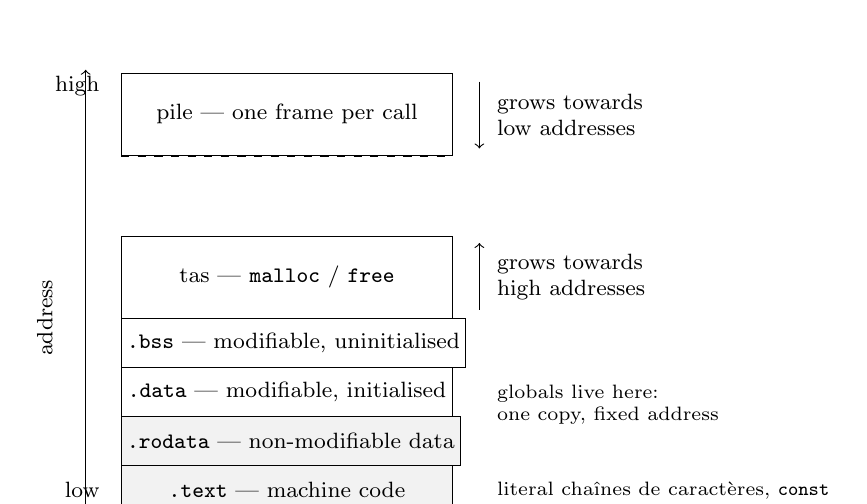
\begin{tikzpicture}[font=\footnotesize]
    \tikzset{seg/.style={draw, minimum width=4.2cm, minimum height=0.62cm,
             anchor=south west, align=center, inner sep=2pt}}
    \node[seg, fill=black!5] at (0,0.00) {\texttt{.text} --- machine code};
    \node[seg, fill=black!5] at (0,0.62) {\texttt{.rodata} --- non-modifiable data};
    \node[seg]               at (0,1.24) {\texttt{.data} --- modifiable, initialised};
    \node[seg]               at (0,1.86) {\texttt{.bss} --- modifiable, uninitialised};
    \node[seg, minimum height=1.05cm] at (0,2.48) {tas --- \texttt{malloc} / \texttt{free}};
    \node[seg, minimum height=1.05cm] at (0,4.55) {pile --- one frame per call};
    \draw[dashed] (0,3.53) -- (4.2,3.53);
    \draw[dashed] (0,4.55) -- (4.2,4.55);
    \draw[->] (4.55,2.60) -- (4.55,3.45);
    \node[right, align=left] at (4.65,3.02) {grows towards\\high addresses};
    \draw[->] (4.55,5.50) -- (4.55,4.65);
    \node[right, align=left] at (4.65,5.08) {grows towards\\low addresses};
    \node[left] at (-0.15,0.31) {low};
    \node[left] at (-0.15,5.45) {high};
    \draw[->] (-0.45,0.10) -- (-0.45,5.65);
    \node[rotate=90, anchor=south] at (-0.75,2.5) {address};
    \node[right, align=left, font=\scriptsize] at (4.65,1.40)
      {globals live here:\\one copy, fixed address};
    \node[right, align=left, font=\scriptsize] at (4.65,0.30)
      {literal chaînes de caractères, \texttt{const}};
  \end{tikzpicture}
\end{figure}

\begin{example}[Divers stockages de variables]
  This example puts one global, one addressed local and one optimised-away
  local in the same function and shows the assembly the compilateur emits.
  \begin{lstlisting}[language=C]
int globale = 123;

int f() {
  int locale = 456;
  int inlinee = 1+g(&locale);
  return inlinee;
}
  \end{lstlisting}
  \begin{lstlisting}[language=gas]
  .text
  .globl f
f:
  subq $24, %rsp
  movl $456, 12(%rsp)    ;;; locale dans 12(%rsp)
  leaq 12(%rsp), %rdi
  call g@PLT
  addl $1, %eax          ;;; inlinee dans %eax
  addq $24, %rsp
  ret
  .globl globale
  .data
globale:                 ;;; globale dans section data car modifiable
  .long 123              ;;; et initialisee
  ;;; dans une section bss si modifiable non initialisee
  ;;; dans une section rodata si non modifiable
  \end{lstlisting}
  Reading the three variables off the listing:
  \begin{center}
  \begin{tabular}{llll}
    \toprule
    Variable & Durée de vie & Where & Evidence \\
    \midrule
    \verb|globale| & the whole program & \verb|.data| & \verb|globale: .long 123| \\
    \verb|locale|  & one call to \verb|f| & the pile, at \verb|12(%rsp)| & \verb|movl $456, 12(%rsp)| \\
    \verb|inlinee| & one call to \verb|f| & the registre \verb|%eax| & \verb|addl $1, %eax| \\
    \bottomrule
  \end{tabular}
  \end{center}
  The \verb|subq $24, %rsp| / \verb|addq $24, %rsp| pair is the frame being
  opened and closed; \verb|locale| occupies four of those twenty-four bytes.
\end{example}

\begin{remark}
  \verb|locale| and \verb|inlinee| are both locals of the same function and yet
  they are stored differently. The discriminating fact is in the source code: the
  program writes \verb|&locale|, so \verb|locale| must have an address, and the
  compilateur is forced to give it a slot on the pile --- hence
  \verb|leaq 12(%rsp), %rdi|, which hands that address to \verb|g|.
  \verb|inlinee| is never addressed, is read once, and is therefore allowed to
  exist only in \verb|%eax|. ``Having an address'' is exactly the valeur gauche
  notion of the next subsection, and it is what decides registre versus pile.
\end{remark}

\subsubsection{Fonctions}
Syntaxe générale :
\begin{lstlisting}[language=C]
type_retour nom_fonction(type1 arg1, type2 arg2) {
   /// code de la fonction
   return valeur_retour;
}
\end{lstlisting}
Précisions : on met usuellement \verb|type_retour = void| si la fonction ne
renvoie rien, et le \verb|return| est facultatif (mais on ne sait alors pas ce
que la fonction renvoie).

\begin{example}
  \begin{lstlisting}[language=C]
int produit(int a, int b) { return a*b; }
int life() { return 42; }
void set(int v) { x=v; }
  \end{lstlisting}
\end{example}

\subsubsection{Expressions}
Les expressions en C sont (entre autres) composées :
\begin{itemize}
  \item des \textbf{constantes} \verb|42|, \verb|0xA2|, \verb|'H'| que l'on
    peut typer (p.~ex.\ \verb|42LL| est $42$ en \verb|long long|);
  \item des \textbf{variables};
  \item de \textbf{sous-expressions parenthésées};
  \item des \textbf{appels de fonctions};
  \item de diverses \textbf{opérations binaires infixes} : \verb|+|, \verb|-|,
    \verb|*|, \verb|/|, \verb|<|, \verb|>|, \verb|<=|, \verb|>=|, \verb|=|,
    \verb|==|, \verb|%|;
  \item de divers \textbf{opérateurs unaires} : \verb|!|, \verb|~|, \verb|-|,
    \verb|*|, \verb|&|, \verb|++|, \verb|--|.
\end{itemize}
Toute expression a un type qui définit la place nécessaire et le comportement.

\begin{remark}
  \verb|=| appears in the list of \textit{opérations binaires}, not in a separate
  list of statements. Assignment is an expression whose value is the value
  assigned, which is what makes \verb|y=(x=42*f(3,5*g(2)))| legal: the inner
  assignment to \verb|x| yields a value, and that value is then stored in
  \verb|y|.
\end{remark}

\begin{example}[Four expressions]
  \begin{center}
  \begin{tabular}{ll}
    \toprule
    Expression & What it does \\
    \midrule
    \verb|y=(x=42*f(3,5*g(2)))| & nested calls; the assignment to \verb|x| returns a value \\
    \verb|x=(1+(2<3))| & \verb|2<3| evaluates to $1$, so \verb|x| becomes $2$ \\
    \verb|0.+1/2| & \verb|1/2| is \textit{integer} division, i.e.\ $0$; the result is $0.0$ \\
    \verb|(0.+1)/2| & \verb|0.+1| is a \verb|double|, so the division is real: $0.5$ \\
    \bottomrule
  \end{tabular}
  \end{center}
  The last two differ only by a pair of parentheses and by a factor of
  infinity in the answer, because the type of a sub-expression --- not the type
  of the variable being assigned --- decides which division is compiled.
\end{example}

\subsubsection{Structures de contrôle}
\begin{lstlisting}[language=C]
while(condition) fairequelquechose

if(condition) fairequelquechose
if(condition) fairequelquechose else fairequelquechose
\end{lstlisting}
Si \verb|fairequelquechose| est composé de plusieurs instructions il faut les
mettre entre accolades. Une condition est \textbf{vraie} si en l'évaluant on
obtient une valeur \textit{différente de} $0$. There is no separate boolean
type to satisfy.

\begin{example}[Collatz]
  \begin{lstlisting}[language=C]
int n = 0; while(n<42) n++;
while(n!=1) {
  if(n%2)        /// teste la parite car n%2=0 <==> n est pair
    n = 3*n+1 ;  /// n est forcement pair maintenant
  n /= 2;
}
  \end{lstlisting}
  The condition \verb|n%2| is used directly as the test: it is $0$ when
  \verb|n| is even and $1$ when it is odd, and no comparison against a boolean
  is written. The comment records the loop's invariant --- after the
  \verb|if| body, \verb|n| is necessarily even, so the unconditional
  \verb|n /= 2| is exact.
\end{example}

\subsection{Pointeurs}
\subsubsection{Valeur gauche}
\begin{definition}[Valeur gauche]
  Une \textbf{valeur gauche} (\textit{left-value}) c'est une valeur qui peut
  être à gauche dans un \verb|=|. En C une valeur gauche c'est une valeur qui
  est \textbf{stockée quelque part en mémoire} (et qui a un type). Autrement
  dit, une valeur gauche c'est quelque chose qui \textbf{a une adresse en
  mémoire}.
\end{definition}

\begin{lstlisting}[language=C]
int a;
a = 42 ; /// autorise
42 = a ; /// interdit, on ne peut pas modifier 42
\end{lstlisting}
\verb|a| est une valeur gauche mais pas \verb|42|. There is no memory cell
called ``\,$42$\,'' to write into.

\subsubsection{Pointeur}
\begin{definition}[Pointeur]
  Un \textbf{pointeur} (\textit{pointer}) est un objet qui stocke l'adresse
  mémoire d'un certain type :
  \begin{itemize}
    \item \verb|T* p| déclare un pointeur \verb|p| vers un objet de type \verb|T|;
    \item \verb|&a| récupère l'adresse d'un objet \verb|a|;
    \item \verb|*p| renvoie l'objet de type \verb|T| pointé par \verb|p|;
    \item \verb|*p| est une valeur gauche car \verb|*p| est stocké à
      l'adresse \verb|p|.
  \end{itemize}
\end{definition}

\begin{remark}
  \verb|&| is the \textit{address-of} or \textit{referencing} operator and
  \verb|*| is the \textit{dereferencing} or \textit{indirection} operator:
  taking \verb|&a| is référencer, evaluating \verb|*p| is déréférencer. The
  operators themselves are unambiguous --- \verb|&| goes from an object to its
  address, \verb|*| goes from an address to the object --- and the two names
  are easy to swap, so read the symbols and not the names.
\end{remark}

\begin{lstlisting}[language=C]
int a, b ;
int * t ;  /// int* c'est un type de pointeur vers un int
t = &a ;   /// t stocke maintenant l'adresse de a
*t = 42 ;
t = &b ; *t = 17;  /// a vaut 42 et b vaut 17
\end{lstlisting}

\begin{figure}[h!]
  \centering
  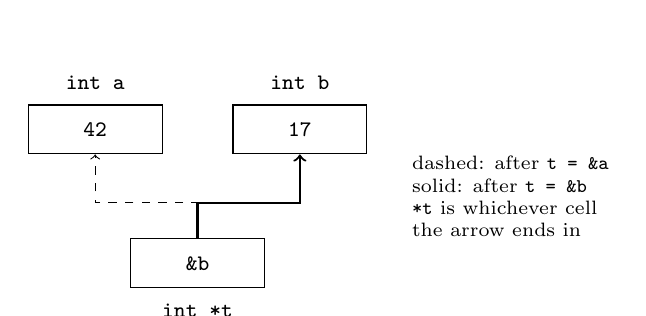
\begin{tikzpicture}[font=\footnotesize]
    \tikzset{cell/.style={draw, minimum width=1.7cm, minimum height=0.62cm}}
    \node[cell] (a) at (0,0)   {\texttt{42}};
    \node[cell] (b) at (2.6,0) {\texttt{17}};
    \node[above=2pt of a] {\texttt{int a}};
    \node[above=2pt of b] {\texttt{int b}};
    \node[cell] (t) at (1.3,-1.7) {\texttt{\&b}};
    \node[below=2pt of t] {\texttt{int *t}};
    \draw[->, thick]  (t.north) -- ++(0,0.45) -| (b.south);
    \draw[->, dashed] (t.north) -- ++(0,0.45) -| (a.south);
    \node[right, align=left, font=\scriptsize] at (3.9,-0.85)
      {dashed: after \texttt{t = \&a}\\solid: after \texttt{t = \&b}\\
       \texttt{*t} is whichever cell\\the arrow ends in};
  \end{tikzpicture}
\end{figure}

Two identities follow directly from the definition, and they are the ones to
recite in an exam.

\begin{prop}[Allers-retours]
  Quand \verb|a| est une valeur gauche, alors
  \begin{center}
    \verb|*(&a) == a|,
  \end{center}
  car \verb|&a| récupère l'adresse de \verb|a| et \verb|*| récupère ensuite la
  valeur à cette adresse. De même si \verb|a| pointe vers quelque chose alors
  \begin{center}
    \verb|&(*a) == a|,
  \end{center}
  car \verb|*a| crée une valeur gauche stockée à l'adresse \verb|a| et \verb|&|
  récupère ensuite l'adresse de la valeur gauche.
\end{prop}

\begin{remark}
  \verb|*a| est \textbf{toujours} une valeur gauche, \verb|&a| ne l'est
  \textbf{jamais}. The asymmetry is the whole content of the previous subsection: \verb|*a|
  names a cell, whereas \verb|&a| is a computed address that is not itself
  stored anywhere. Hence \verb|*p = 42| compiles and \verb|&a = 42| does not.
\end{remark}

\subsubsection{Arithmétique de pointeurs}
Le type des pointeurs change le comportement de l'arithmétique. For
\verb|p|, \verb|p1|, \verb|p2| of type \verb|T*| and \verb|i| an integer:
\begin{align*}
  p + i &\;\Longleftrightarrow\; p + \mathtt{sizeof}(T) \times i, \\
  p - i &\;\Longleftrightarrow\; p - \mathtt{sizeof}(T) \times i, \\
  p_1 - p_2 &\;\Longleftrightarrow\; (p_1 - p_2) \,/\, \mathtt{sizeof}(T)
    \qquad \text{for } p_1,\, p_2 \text{ of the same type } \text{\texttt{T*}}, \\
  \text{\texttt{p++}} &\;\Longleftrightarrow\; p = p + 1.
\end{align*}
Les opérations qui n'ont pas de sens échouent : $p_1 + p_2$, $p_1 * p_2$,
etc. Adding two addresses names nothing, whereas subtracting two addresses of
the same type names a count of elements.

\begin{remark}
  The scaling is silent. Si \verb|t| pointe vers un entier 4 octets,
  \verb|t+1| vers l'entier \textit{d'après} qui est 4 octets plus loin. The
  source code reads \verb|t+1| and the machine computes
  $\verb|t| + 4$. This is also why \verb|void *| arithmetic is ill-defined:
  \verb|sizeof(void)| is ``$1$ mais mal défini''.
\end{remark}

\subsubsection{Tableaux}
Les tableaux sont \textbf{presque que des pointeurs} :

\begin{lstlisting}[language=C]
int t[5] = {1,2,3,4,5} ;
int * x = t;
*x = 1 ;       /// modifie t[0]
*(x+2) = 2 ;   /// modifie t[2]
\end{lstlisting}

\begin{prop}[L'indexation est du sucre syntaxique]
  En C, \verb|t[i]| est du \textbf{sucre syntaxique} (\textit{syntactic sugar})
  pour
  \[ \verb|*(t+i)|. \]
\end{prop}

\begin{remark}
  \verb|+| is commutative, so \verb|*(t+i)| is \verb|*(i+t)|. On peut
  d'ailleurs écrire \verb|4[t]| plutôt que \verb|t[4]|. It compiles. The
  bracket is therefore not a primitive operation on a special ``array'' object
  but a règle de réécriture on a pointeur and an integer.
\end{remark}

L'initialisation de la forme \verb|int t[10]| marche quand on connaît la taille
du tableau. Cela réserve $10 \times \verb|sizeof(int)|$ octets. Si on ne
connaît \textit{pas} la taille du tableau à la compilation il faut demander de
la mémoire à l'OS. Il y a une fonction dans la libC qui gère l'allocation
mémoire : \verb|malloc|.

\begin{lstlisting}[language=C]
int * t = malloc(40) ;
  /// 40 octets, soit 10 int de taille 4

t = malloc( 10 * sizeof(int) ) ; /// autre maniere
/// de demander la meme chose
\end{lstlisting}

\begin{remark}
  The two calls request the same thing, but only the second survives a change
  of architecture: the literal \verb|40| silently assumes
  \verb|sizeof(int) == 4|, which the table of types above gives as only
  \textit{souvent} true. Write the \verb|sizeof| form.
\end{remark}

\subsubsection{Chaînes de caractères}
En C, les caractères sont de type \verb|char| et les \textbf{chaînes de
caractères} (\textit{strings}) sont simplement des tableaux de caractères, et
des pointeurs \verb|char*|. Une chaîne de la forme \verb|"machaine"| dans le
programme C est une valeur de type \verb|const char *|.

\begin{notation}
  Par convention, une chaîne de caractères se termine par le caractère
  \verb|'\0'| dont la valeur numérique est $0$. Nothing else records the
  length: the terminator \textit{is} the length.
\end{notation}

\begin{lstlisting}[language=C]
const char * s = "Hello World!"; /// C rajoute un '\0'
int len = 0 ;
while(s[len])  /// s'arrete quand s[len] vaut 0 = '\0'
  len++;
s[2] = '?' ;   /// que va faire cette ligne ?
\end{lstlisting}

\begin{remark}
  The loop needs no comparison: \verb|s[len]| is itself the condition, and it
  is false exactly on the terminator, since a condition is true when it differs
  from $0$ and \verb|'\0'| \textit{is} $0$. On exit, \verb|len| is the number of
  characters before the terminator.
\end{remark}

\begin{remark}
  The listing's last line is left as a question. Two independent things are
  wrong with \verb|s[2] = '?'|. The type of \verb|s| is \verb|const char *|, so
  the pointed-to object is declared non-modifiable and the compilateur objects.
  And by the storage rules above, non-modifiable data goes in \verb|.rodata|, a
  section the loader maps read-only --- so forcing the write past the
  compilateur gets it refused by the hardware at run time rather than executed.
\end{remark}

\subsection{Bibliothèque C}
\begin{definition}[libC]
  La \textbf{libC} (pour C library et donc bibliothèque C) est un ensemble de
  fonctions qui permettent à C d'interagir avec l'OS \textit{quel que soit}
  l'OS. It is the portability layer: the C program calls libC, and libC calls
  whichever system interface the platform actually has.
\end{definition}

La libC contient beaucoup de fonctions, vous devez en connaître 4 :
\begin{center}
\begin{tabular}{ll}
  \toprule
  Function & Role \\
  \midrule
  \verb|malloc| & alloue de la mémoire (déjà vue) \\
  \verb|free|   & libère de la mémoire allouée par \verb|malloc| \\
  \verb|printf| & affiche sur la sortie standard \\
  \verb|scanf|  & lit sur l'entrée standard \\
  \bottomrule
\end{tabular}
\end{center}

\subsubsection{printf}
La fonction \verb|printf| prend un nombre arbitraire de paramètres et le premier
paramètre est un \textbf{format} de type chaîne de caractères. The format is
copied to the output verbatim except at the \verb|%| placeholders, each of
which consumes one further argument.

\begin{example}
  \begin{lstlisting}[language=C]
printf("Hello World!");
printf("%d",42);
printf("%s","Hello World");
printf("a=%d / b=%d / chaine %s", 1, 2, "coucou");
\end{lstlisting}
  The last line is the general case: several arguments interleaved with literal
  text, consumed left to right in the order the placeholders appear.
\end{example}

\paragraph{Formats utiles}
Voici les formats qui peuvent être utiles dans ce cours :
\begin{center}
\begin{tabular}{lll}
  \toprule
  Format & Argument & Size of the argument \\
  \midrule
  \verb|%d|   & entier décimal sous forme de \verb|int| & souvent 4 octets \\
  \verb|%lld| & entier décimal sous forme de \verb|long long| & 8 octets \\
  \verb|%s|   & chaîne de caractères (pointeur vers le premier caractère) & 8 octets \\
  \verb|%c|   & affiche un unique caractère & --- \\
  \verb|%p|   & affiche l'adresse d'un pointeur & 8 octets \\
  \bottomrule
\end{tabular}
\end{center}

\begin{remark}
  \textbf{Attention} : pour \verb|printf| il faut faire attention à ce que
  \textit{les tailles des types soient les bonnes}. \verb|printf| is variadic:
  it cannot inspect what it was handed, so it reads as many bytes off the
  argument area as the format tells it to. Passing a \verb|long long| to
  \verb|%d| or an \verb|int| to \verb|%lld| makes \verb|printf| read the wrong
  number of bytes for that placeholder and print garbage; on ABIs that pass
  variadic arguments on the pile it additionally shifts every later argument.
  The compilateur has no type to check against. This is the practical face of
  ``le type n'existe qu'au moment de la compilation''.
\end{remark}

\subsubsection{scanf}
La fonction \verb|scanf| est similaire à \verb|printf| excepté qu'elle
\textit{lit}. Les arguments ne sont pas tout à fait les mêmes car \verb|printf|
prend des \textbf{valeurs}, \verb|scanf| doit prendre des \textbf{pointeurs} :
\begin{itemize}
  \item pour lire une chaîne de caractères, ça ne change pas le type, on passe
    un pointeur où l'on veut que \verb|scanf| stocke la chaîne (comme
    \verb|printf|);
  \item pour lire un entier, on passe un pointeur où stocker l'entier.
\end{itemize}

\begin{lstlisting}[language=C]
char chaine_lue[100] ;
int entier_lu ;
scanf("%s %d",chaine_lue, &entier_lu);
/// en lisant une chaine avec %s scanf s'arrete a la premiere espace ' ',
/// tabulation '\t' ou retour a la ligne '\n'
/// avec %d l'entier doit etre decimal (%i pour octal ou hexadecimal)
\end{lstlisting}

\begin{remark}
  \verb|chaine_lue| is passed bare and \verb|entier_lu| is passed as
  \verb|&entier_lu|. That is not an inconsistency: the array name already
  \textit{is} the address of its first element, so it is already the pointeur
  \verb|scanf| wants, whereas \verb|entier_lu| is an \verb|int| and needs the
  \verb|&|. Reading \verb|t[i]| as \verb|*(t+i)| makes this automatic.
\end{remark}

\begin{remark}
  Two behaviours of the format worth keeping. First, \verb|%s| s'arrête à la
  première espace \verb|' '|, tabulation \verb|'\t'| ou retour à la ligne
  \verb|'\n'|, so it reads one word and not one line. Second, avec \verb|%d|
  l'entier doit être \textit{décimal} (\verb|%i| pour octal ou hexadécimal, as
  well as decimal).
\end{remark}

\subsection{Tableaux}
\subsubsection{Tableaux 2D}
Une solution avec \texttt{malloc} : an array of pointeurs to arrays.

\begin{lstlisting}[language=C]
int ** t ;
/// un pointeur vers des
/// pointeurs vers des entiers

t = malloc( sizeof(int*) * 10 ) ;
/// attention sizeof(int*) !

int i = 0;
while(i<10) {
  t[i] = malloc( sizeof(int) * 10 ) ;
  i++;
}
\end{lstlisting}

\begin{figure}[h!]
  \centering
  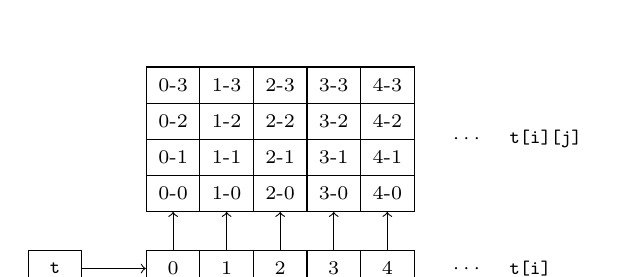
\begin{tikzpicture}[font=\scriptsize]
    \tikzset{c/.style={draw, minimum width=0.68cm, minimum height=0.46cm, inner sep=1pt}}
    \foreach \i in {0,...,4} {
      \node[c] (p\i) at (\i*0.68,0) {\i};
      \foreach \j in {0,...,3} {
        \node[c] at (\i*0.68, 0.95+\j*0.46) {\i-\j};
      }
      \draw[->] (\i*0.68,0.23) -- (\i*0.68,0.72);
    }
    \node at (3.75,0) {$\cdots$};
    \node at (3.75,1.65) {$\cdots$};
    \node[c] (root) at (-1.5,0) {\texttt{t}};
    \draw[->] (root.east) -- (p0.west);
    \node[right] at (4.15,1.65) {\texttt{t[i][j]}};
    \node[right] at (4.15,0)    {\texttt{t[i]}};
  \end{tikzpicture}
\end{figure}

\begin{remark}
  \textit{Attention} \verb|sizeof(int*)| in the first \verb|malloc|: the outer
  allocation holds \textit{pointeurs}, 8 bytes each, not integers. Writing
  \verb|sizeof(int)| there would reserve half the memory needed and corrupt the
  spine of the structure.
\end{remark}

\begin{remark}
  C'est le même fonctionnement en OCaml et en Python : un tableau
  multidimensionnel est un \textbf{tableau de tableaux}. The rows are separate
  allocations, so they need not be contiguous with one another and need not
  even have the same length.
\end{remark}

\subsubsection{Tableaux linéarisés}
The other solution is the built-in multidimensional array, which is not an
array of arrays at all.

\begin{lstlisting}[language=C]
int t[99][88][77] ; /// en fait c'est un tableau de taille 99x88x77

int i =3, j=4, k=5;
t[i][j][k] /// est remplace par *(t+i*88*77+j*77+k)
\end{lstlisting}

A single block of $99 \times 88 \times 77$ integers is reserved, and the
indices are folded into one offset. The compilateur turns
\begin{center}
  \verb|t[i][j][k]| $\longrightarrow$ \verb|*(t + i*88*77 + j*77 + k)|,
\end{center}
where the offset is counted in \textit{elements} --- the scaling by
\verb|sizeof(int)| is then supplied by the arithmétique de pointeurs of the
previous subsection. Note which dimensions appear: the first, $99$, does not, while
$88$ and $77$ do.

\begin{figure}[h!]
  \centering
  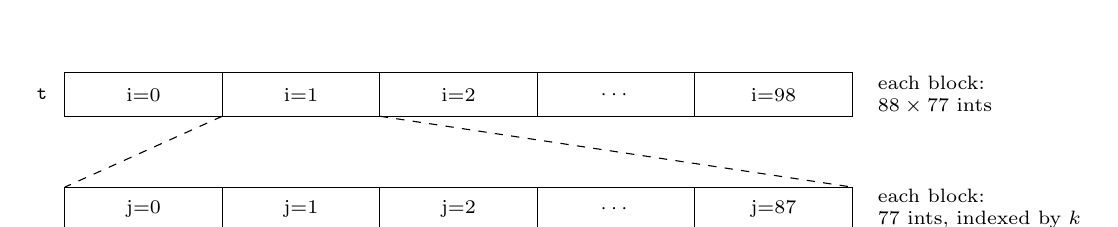
\begin{tikzpicture}[font=\scriptsize]
    % top strip: the i-blocks
    \draw (0,0) rectangle (10,0.55);
    \foreach \x in {2,4,6,8} \draw (\x,0) -- (\x,0.55);
    \foreach \x/\l in {1/{i=0}, 3/{i=1}, 5/{i=2}, 7/{$\cdots$}, 9/{i=98}}
      \node at (\x,0.275) {\l};
    \node[left] at (-0.1,0.275) {\texttt{t}};
    \node[right, align=left] at (10.2,0.275) {each block:\\$88\times 77$ ints};
    % guides
    \draw[dashed] (2,0) -- (0,-0.9);
    \draw[dashed] (4,0) -- (10,-0.9);
    % bottom strip: the j-blocks inside one i-block
    \draw (0,-1.45) rectangle (10,-0.9);
    \foreach \x in {2,4,6,8} \draw (\x,-1.45) -- (\x,-0.9);
    \foreach \x/\l in {1/{j=0}, 3/{j=1}, 5/{j=2}, 7/{$\cdots$}, 9/{j=87}}
      \node at (\x,-1.175) {\l};
    \node[right, align=left] at (10.2,-1.175) {each block:\\$77$ ints, indexed by $k$};
  \end{tikzpicture}
\end{figure}

\begin{remark}
  Le type tableau multidimensionnel est un pointeur avec l'information
  additionnelle des dimensions (sauf la première) et un peu compliqué
  à comprendre. Il vaut mieux éviter de faire des choses compliquées avec. The
  first dimension is absent because it is never needed to compute an offset
  --- only the strides below a given index matter.
\end{remark}

\begin{example}[Passing a slice]
  \begin{lstlisting}[language=C]
void f(int a[][77]) { a[2][3] = 42 ; } /// a est un pointeur
int (*x)[88][77] = t;
f(x[1]); /// calcule x+1*sizeof(int[88][77]) = 88*77*4
  \end{lstlisting}
  The parameter \verb|int a[][77]| is a pointeur that remembers the stride
  $77$, which is all \verb|a[2][3]| needs: the offset is $2 \times 77 + 3$
  elements. The variable \verb|x| is a pointeur to an \verb|int[88][77]|, so
  \verb|x[1]| advances by one whole $88 \times 77$ slab --- the comment records
  the arithmetic as $88 \times 77 \times 4$ bytes, the factor $4$ being
  \verb|sizeof(int)|.
\end{example}

\begin{conclusion}
  The two constructions have the same indexing syntax and nothing else in
  common. \verb|int **t| is one allocation of pointeurs plus one allocation per
  row: \verb|t[i][j]| costs two memory reads, the rows are independent, and
  \verb|free| must be called once per row plus once for the spine.
  \verb|int t[99][88][77]| is a single contiguous block: \verb|t[i][j][k]| costs
  one multiply-add and one read, nothing is separately allocated, and the
  dimensions are baked into the type. Knowing which one is in front of you is
  the difference between an offset computation and a chase from pointeur to
  pointeur.
\end{conclusion}

\section{Fonctions, la pile et la libC}
The machine has no notion of a function. It has registres, a flat array of bytes
and a program counter, and that is all. Everything that makes a function ---
parameters, local variables, a valeur de retour, the guarantee that the
appelant's data survives the call --- is an agreement between two pieces of code
that never meet. This chapter states that agreement. It begins with the memory a
processus is given, narrows to the region that agreement lives in (the pile),
then fixes the System V calling convention that \texttt{gcc} and the libC both
obey, and ends by calling \texttt{scanf} and \texttt{printf} from bare assembly.

\subsection{Organisation de la mémoire}
\begin{definition}[Les trois parties de la mémoire d'un programme]
  En simplifiant beaucoup, la mémoire d'un programme est composée de trois
  parties :
  \begin{itemize}
    \item la \textbf{mémoire statique} (\textit{static memory}) chargée par l'OS
      depuis l'ELF (le contenu des sections \texttt{.text}, \texttt{.data},
      \texttt{.bss}, etc.) ;
    \item la \textbf{pile} (\textit{stack}), qui est une mémoire fournie par
      l'OS \emph{pour les fonctions} ; l'OS fournit directement cette mémoire ;
    \item le \textbf{tas} (\textit{heap}), qui est une mémoire fournie par l'OS
      \emph{sur demande}.
  \end{itemize}
\end{definition}

The distinction that matters for this chapter is the second one. The mémoire
statique is fixed at the édition de liens and the tas has to be requested
(through \texttt{malloc}, i.e.\ ultimately through a system call); the pile is
simply \emph{there} when the processus starts, without being asked for, which is
why a function can allocate its working space in a single subtraction and free
it in a single addition.

\begin{figure}[h!]
  \centering
  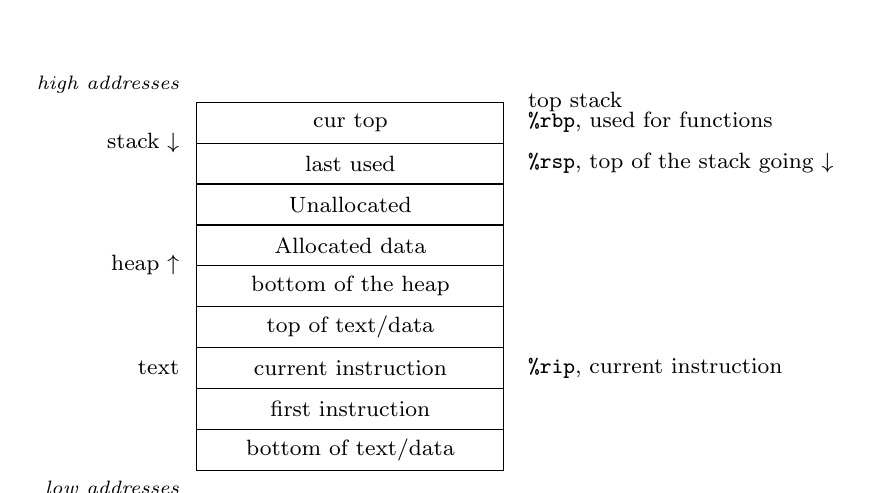
\begin{tikzpicture}[font=\footnotesize]
    \tikzset{
      cell/.style={draw, minimum width=3.9cm, minimum height=0.52cm,
                   inner sep=1pt, anchor=north},
      ann/.style={anchor=west, xshift=5pt},
    }
    \node[cell] (ra) at (0, 0.00) {cur top};
    \node[cell] (rb) at (0,-0.52) {last used};
    \node[cell] (rc) at (0,-1.04) {Unallocated};
    \node[cell] (rd) at (0,-1.56) {Allocated data};
    \node[cell] (re) at (0,-2.08) {bottom of the heap};
    \node[cell] (rf) at (0,-2.60) {top of text/data};
    \node[cell] (rg) at (0,-3.12) {current instruction};
    \node[cell] (rh) at (0,-3.64) {first instruction};
    \node[cell] (ri) at (0,-4.16) {bottom of text/data};

    \node[ann] at (ra.north east) {top stack};
    \node[ann] at (ra.east) {\texttt{\%rbp}, used for functions};
    \node[ann] at (rb.east) {\texttt{\%rsp}, top of the stack going $\downarrow$};
    \node[ann] at (rg.east) {\texttt{\%rip}, current instruction};

    \node[anchor=east] at (-2.05,-0.52) {stack $\downarrow$};
    \node[anchor=east] at (-2.05,-2.08) {heap $\uparrow$};
    \node[anchor=east] at (-2.05,-3.38) {text};

    \node[anchor=east, font=\scriptsize\itshape] at (-2.05, 0.22) {high addresses};
    \node[anchor=east, font=\scriptsize\itshape] at (-2.05,-4.90) {low addresses};
  \end{tikzpicture}
\end{figure}

Read the picture from the bottom: the text and data loaded from the ELF sit at
the low addresses, the tas grows \emph{upwards} from just above them, and the
pile grows \emph{downwards} from the top. Between the two lies unallocated
address space, which is what lets both grow. Three registres point into this
picture: \texttt{\%rip} into the text at the current instruction, \texttt{\%rsp}
at the top of the pile, and \texttt{\%rbp} somewhat higher up in the pile,
``used for functions''.

\subsubsection{Organisation de la pile pour les fonctions}
\begin{definition}[Organisation de la pile pour les fonctions (\textit{stack discipline})]
  Il est \emph{standard} --- not enforced by the hardware --- que :
  \begin{itemize}
    \item \textbf{presque toujours}, \texttt{\%rsp} pointe vers le premier
      octet utilisé de la pile ;
    \item \textbf{souvent} \texttt{\%rbp} pointe vers le début de la pile au
      début de l'appel de la fonction courante.
  \end{itemize}
\end{definition}

\begin{remark}
  The hedging is worth keeping. ``Presque toujours'' and ``souvent'' are the
  right words because nothing in the processor checks either claim:
  \texttt{\%rsp} and \texttt{\%rbp} are ordinary registres généraux. Only the
  instructions \texttt{push}, \texttt{pop}, \texttt{call} and \texttt{ret} ---
  and the interrupt machinery --- treat \texttt{\%rsp} specially.
  \texttt{\%rbp} is special to nobody at all; it is a convention kept by
  compilateurs.
\end{remark}

\paragraph{Manipuler la pile}
Les commandes suivantes permettent de manipuler la pile :
\begin{itemize}
  \item \texttt{push \%rbx} ou \texttt{pushq \$42} décale \texttt{\%rsp} de la
    bonne taille puis stocke \texttt{\%rbx}/\texttt{42} dans \texttt{(\%rsp)} ;
  \item \texttt{pop \%rbx} récupère la valeur \texttt{(\%rsp)} dans
    \texttt{\%rbx} puis décale \texttt{\%rsp} de la bonne taille.
\end{itemize}
Ces commandes peuvent s'écrire autrement (\texttt{add} + \texttt{mov}). Since
the pile grows towards the low addresses, ``décale \texttt{\%rsp} de la bonne
taille'' means \emph{subtracting} the operand size on a push and \emph{adding}
it on a pop:

\begin{lstlisting}[language=gas]
        pushq   %rbx            # is the pair
        subq    $8, %rsp
        movq    %rbx, (%rsp)

        popq    %rbx            # is the pair
        movq    (%rsp), %rbx
        addq    $8, %rsp
\end{lstlisting}

\begin{remark}
  Note the order inside each pair: a push decrements \emph{then} writes, a pop
  reads \emph{then} increments. \texttt{(\%rsp)} therefore always denotes a byte
  that is in use, never free space. Note also that the two halves are ordinary
  instructions, so nothing stops you from moving \texttt{\%rsp} by hand:
  \texttt{subq \$32, \%rsp} allocates thirty-two bytes in one stroke, which is
  exactly what a function prologue does, and is far cheaper than four pushes.
\end{remark}

\subsection{Fonctions en assembleur}
\begin{definition}[Les fonctions ne sont que des conventions]
  \emph{En assembleur les fonctions ne sont que des conventions.} In assembly a
  function is not a language construct; it is a pair of promises, one kept by
  the code that calls, the \textbf{appelant} (\textit{caller}), and one kept by
  the code that is called, the \textbf{fonction appelée} (\textit{callee}), about
  where arguments live, where the result is left, which registres survive, and
  where execution resumes.
\end{definition}

\subsubsection{L'appelant}
Avant d'appeler une fonction, \texttt{gcc} va :
\begin{itemize}
  \item sauvegarder les registres que la fonction appelée risque d'écraser ;
  \item stocker les arguments à des endroits prédéfinis (p.~ex.\ sur les
    registres puis la pile) ;
  \item stocker l'adresse de l'instruction à exécuter une fois que la fonction
    termine ;
  \item sauter au début de la fonction ;
  \item en revenant, retirer les arguments mis sur la pile ;
  \item restaurer la valeur des registres sauvegardés.
\end{itemize}
The third and fourth steps together are precisely what the \texttt{call}
instruction does; the rest is code the compilateur emits around it.

\subsubsection{La fonction appelée}
Pour une fonction appelée, \texttt{gcc} va :
\begin{itemize}
  \item allouer une \textbf{frame} et sauvegarder le \texttt{\%rbp} précédent ;
  \item faire le calcul ;
  \item libérer la frame ;
  \item revenir à l'appelant.
\end{itemize}
The first item is the \textbf{prologue}, the last two the \textbf{epilogue}.

\subsubsection{Quelques commandes utiles pour les fonctions}
\begin{center}
  \begin{tabularx}{\textwidth}{lX}
    \toprule
    instruction & effect \\
    \midrule
    \texttt{call label} &
      plus ou moins équivalent à \texttt{push \%rip+8} combiné à
      \texttt{jmp label} \\
    \texttt{ret} &
      plus ou moins équivalent à \texttt{pop \%rip} \\
    \texttt{enter 32} &
      équivalent à \texttt{pushq \%rbp}, \texttt{movq \%rsp, \%rbp},
      \texttt{subq \$32, \%rsp}, mais n'est généralement pas utilisé \\
    \texttt{leave} &
      équivalent à \texttt{movq \%rbp, \%rsp}, \texttt{pop \%rbp}, un peu plus
      souvent utilisé \\
    \bottomrule
  \end{tabularx}
\end{center}

\begin{remark}
  The ``plus ou moins'' in the first two rows is essential. \texttt{\%rip} is not
  an addressable registre général on x86-64: \texttt{push \%rip} and
  \texttt{pop \%rip} are not instructions you can assemble. The equivalence
  describes the \emph{effect} --- \texttt{call} pushes the return address and
  transfers control, \texttt{ret} pops it back into the program counter --- not
  a rewriting you may type. The \texttt{+8} likewise stands for ``the length of
  the \texttt{call} instruction''; what is pushed is the address of the
  instruction that follows the \texttt{call}.
\end{remark}

\begin{remark}
  \texttt{enter} and \texttt{leave} are single instructions that package a
  whole prologue and epilogue. \texttt{enter} is slow enough on modern
  processors that compilateurs avoid it; \texttt{leave} survives because it is
  one byte and does exactly the right thing.
\end{remark}

\subsubsection{La frame}
The standard prologue and epilogue, written out longhand, are
\begin{lstlisting}[language=gas]
f:      pushq   %rbp            # save the caller's frame pointer
        movq    %rsp, %rbp      # this frame starts here
        subq    $32, %rsp       # 32 bytes of local variables
        # ... the computation ...
        movq    %rbp, %rsp      # free the frame  (these two lines = leave)
        popq    %rbp
        ret
\end{lstlisting}
so that \texttt{enter 32} replaces the first three lines and \texttt{leave}
replaces the two that free the frame.

\begin{figure}[h!]
  \centering
  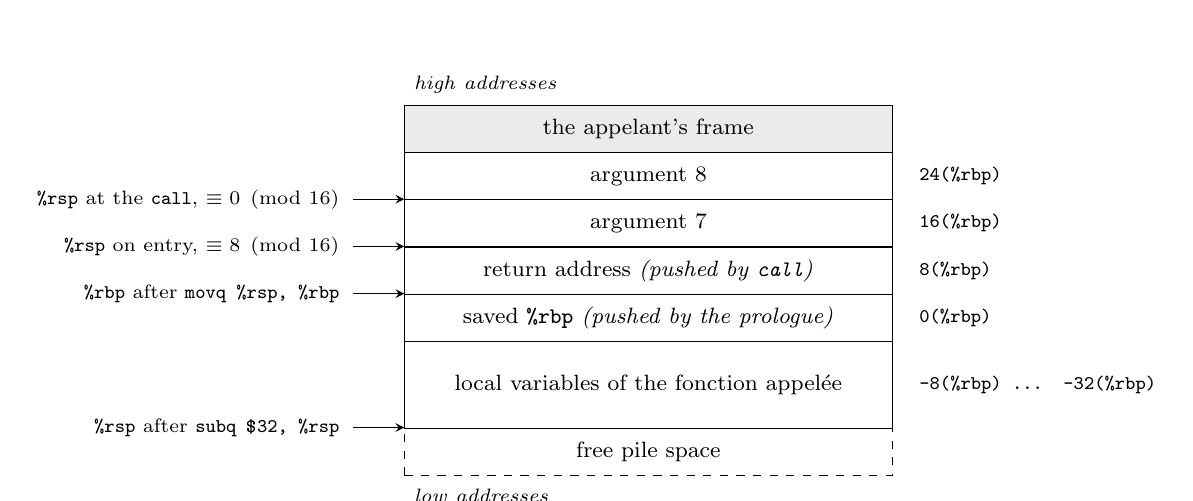
\begin{tikzpicture}[font=\footnotesize, >=stealth]
    \tikzset{
      cell/.style={draw, minimum width=6.2cm, inner sep=2pt, anchor=north},
      lab/.style={anchor=east, font=\scriptsize},
      off/.style={anchor=west, xshift=6pt, font=\scriptsize\ttfamily},
    }
    \node[cell, minimum height=0.6cm, fill=black!8] (c0) at (0, 0.00) {the appelant's frame};
    \node[cell, minimum height=0.6cm] (c1) at (0,-0.60) {argument 8};
    \node[cell, minimum height=0.6cm] (c2) at (0,-1.20) {argument 7};
    \node[cell, minimum height=0.6cm] (c3) at (0,-1.80) {return address \emph{(pushed by \texttt{call})}};
    \node[cell, minimum height=0.6cm] (c4) at (0,-2.40) {saved \texttt{\%rbp} \emph{(pushed by the prologue)}};
    \node[cell, minimum height=1.1cm] (c5) at (0,-3.00) {local variables of the fonction appelée};
    \node[cell, minimum height=0.6cm, dashed] (c6) at (0,-4.10) {free pile space};

    \node[off] at (c1.east) {24(\%rbp)};
    \node[off] at (c2.east) {16(\%rbp)};
    \node[off] at (c3.east) {8(\%rbp)};
    \node[off] at (c4.east) {0(\%rbp)};
    \node[off] at (c5.east) {-8(\%rbp) ... -32(\%rbp)};

    \draw[->] (-3.75,-1.20) -- (-3.10,-1.20);
    \node[lab] at (-3.80,-1.20) {\texttt{\%rsp} at the \texttt{call}, $\equiv 0 \pmod{16}$};
    \draw[->] (-3.75,-1.80) -- (-3.10,-1.80);
    \node[lab] at (-3.80,-1.80) {\texttt{\%rsp} on entry, $\equiv 8 \pmod{16}$};
    \draw[->] (-3.75,-2.40) -- (-3.10,-2.40);
    \node[lab] at (-3.80,-2.40) {\texttt{\%rbp} after \texttt{movq \%rsp, \%rbp}};
    \draw[->] (-3.75,-4.10) -- (-3.10,-4.10);
    \node[lab] at (-3.80,-4.10) {\texttt{\%rsp} after \texttt{subq \$32, \%rsp}};

    \node[anchor=west, font=\scriptsize\itshape] at (-3.10, 0.26) {high addresses};
    \node[anchor=west, font=\scriptsize\itshape] at (-3.10,-4.96) {low addresses};
  \end{tikzpicture}
\end{figure}

Once \texttt{\%rbp} has been set, every interesting slot has a fixed offset from
it, and those offsets stay valid no matter how much \texttt{\%rsp} subsequently
moves. That is the whole point of keeping a pointeur to the frame:
\texttt{0(\%rbp)} holds the appelant's saved \texttt{\%rbp}, \texttt{8(\%rbp)}
the return address,
\texttt{16(\%rbp)} the seventh argument if there is one, and the local variables
live at the negative offsets \texttt{-8(\%rbp)}, \texttt{-16(\%rbp)} and so on.
Addressing the same locals off \texttt{\%rsp} would require recomputing every
offset after each push.

\subsection{La convention d'appel}
The ``endroits prédéfinis'' of the appelant's second step are not a free choice.
On Linux they are fixed by the \textbf{System V AMD64 ABI}, which is the
convention \texttt{gcc} emits and the libC expects. Assembly that calls the libC
must obey it exactly; assembly that only calls itself may do as it pleases, but
there is no reason to invent a second convention. Naming the ABI and its
registres goes beyond this course, which says only that the arguments are stored
\textit{à des endroits prédéfinis} and that one must make \textit{des appels
alignés sur des multiples de 16}. This subsection fills those two phrases in
from the ABI itself.

\subsubsection{Où vont les arguments}
\begin{definition}[Registres d'argument (\textit{argument registers}), dans l'ordre]
  Arguments that are integers or pointeurs are passed in the registres
  \[
    \texttt{\%rdi},\quad \texttt{\%rsi},\quad \texttt{\%rdx},\quad
    \texttt{\%rcx},\quad \texttt{\%r8},\quad \texttt{\%r9}
  \]
  in that order; the seventh and later integer arguments are pushed on the
  pile. Floating-point arguments go in \texttt{\%xmm0} through
  \texttt{\%xmm7}. The two sequences are consumed independently.
\end{definition}

\begin{center}
  \begin{tabular}{lcccccccc}
    \toprule
    argument $n$ & 1 & 2 & 3 & 4 & 5 & 6 & 7 & 8 \\
    \midrule
    integer / pointeur &
      \texttt{\%rdi} & \texttt{\%rsi} & \texttt{\%rdx} & \texttt{\%rcx} &
      \texttt{\%r8} & \texttt{\%r9} & pile & pile \\
    floating point &
      \texttt{\%xmm0} & \texttt{\%xmm1} & \texttt{\%xmm2} & \texttt{\%xmm3} &
      \texttt{\%xmm4} & \texttt{\%xmm5} & \texttt{\%xmm6} & \texttt{\%xmm7} \\
    \bottomrule
  \end{tabular}
\end{center}

The arguments passed on the pile are laid out so that the seventh sits at the
\emph{lowest} address, that is, at \texttt{(\%rsp)} at the instant the
\texttt{call} executes, the eighth at \texttt{8(\%rsp)}, and so on. They are the
appelant's property: removing them after the call is the appelant's fifth step,
and it is one addition to \texttt{\%rsp}.

\begin{definition}[Valeur de retour (\textit{return value})]
  The result comes back in \texttt{\%rax} (in the pair
  \texttt{\%rdx}:\texttt{\%rax} for a 128-bit value) for integers and pointeurs,
  and in \texttt{\%xmm0} for floating point.
\end{definition}

\begin{definition}[\texttt{\%al} et fonctions variadiques]
  For a \textbf{fonction variadique} (\textit{variadic function}) --- one
  declared with \texttt{\dots}, such as \texttt{printf} and \texttt{scanf} ---
  the appelant must additionally set \texttt{\%al} to the number of vector
  (\texttt{\%xmm}) registres used to pass arguments.
\end{definition}

This is what the line \texttt{mov \$0, \%rax} does in every libC example below.
It is not decoration and it is not a cleared valeur de retour: it announces ``no
floating-point argument was passed''. A fonction variadique uses the count to
decide whether it must spill the eight \texttt{\%xmm} registres into its save
area for registres; leaving \texttt{\%rax} holding garbage makes \texttt{printf}
read vector registres it was never given, and the call may fault.

\subsubsection{Questions d'alignement}
\begin{definition}[Alignement (\textit{alignment}) naturel]
  Quand on lit un bloc de taille $2^{k}$, le processeur s'attend à ce que
  l'adresse lue soit un multiple de $2^{k}$.
\end{definition}
Pour \texttt{movq}, \texttt{movl}, \texttt{movw}, \texttt{movb} et toutes les
instructions vues jusqu'à présent ce n'est pas un problème, mais il existe des
instructions qui \emph{s'attendent} à des adresses alignées. x86 tolerates
misaligned ordinary loads and stores, at a speed penalty; the instructions that
expect aligned addresses fault otherwise. Même si vos instructions ignorent
l'alignement, la libC peut l'attendre, il faut donc faire des appels alignés sur
des multiples de $16$.

\begin{definition}[La règle des 16 octets avant un \texttt{call}]
  At the instant the \texttt{call} instruction executes, \texttt{\%rsp} must be
  a multiple of $16$. Since \texttt{call} then pushes an eight-byte return
  address, on entry to the fonction appelée
  \[
    \texttt{\%rsp} \equiv 8 \pmod{16},
  \]
  and the fonction appelée's own \texttt{pushq \%rbp} brings it back to a
  multiple of $16$.
\end{definition}

\begin{figure}[h!]
  \centering
  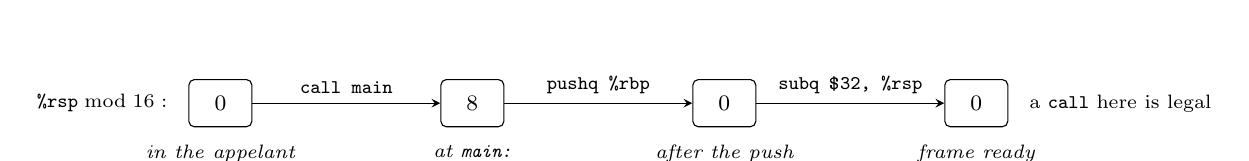
\begin{tikzpicture}[font=\footnotesize, >=stealth]
    \tikzset{
      st/.style={draw, rounded corners=2pt, minimum width=0.8cm,
                 minimum height=0.6cm, inner sep=2pt},
      op/.style={above, font=\scriptsize\ttfamily},
      frmcap/.style={below=3pt, font=\scriptsize\itshape},
    }
    \node[st] (A) at (0.0,0) {$0$};
    \node[st] (B) at (3.2,0) {$8$};
    \node[st] (C) at (6.4,0) {$0$};
    \node[st] (D) at (9.6,0) {$0$};

    \draw[->] (A) -- node[op]{call main} (B);
    \draw[->] (B) -- node[op]{pushq \%rbp} (C);
    \draw[->] (C) -- node[op]{subq \$32, \%rsp} (D);

    \node[frmcap] at (A.south) {in the appelant};
    \node[frmcap] at (B.south) {at \texttt{main:}};
    \node[frmcap] at (C.south) {after the push};
    \node[frmcap] at (D.south) {frame ready};

    \node[anchor=east, font=\scriptsize] at (-0.55,0) {$\texttt{\%rsp} \bmod 16:$};
    \node[anchor=west, font=\scriptsize] at (10.15,0) {a \texttt{call} here is legal};
  \end{tikzpicture}
\end{figure}

\begin{remark}
  Two corollaries that the exercises trip over. First, the frame size must be a
  multiple of $16$: after the entry offset of $8$ and the eight-byte
  \texttt{pushq \%rbp}, \texttt{subq \$32, \%rsp} preserves the alignement
  because $32 \equiv 0 \pmod{16}$, whereas \texttt{subq \$24, \%rsp} would
  destroy it and the next \texttt{call printf} would be misaligned. This is the
  meaning of the warning \textit{``attention gcc peut attendre un alignement 16
  octets''} in the libC skeleton below. Second, an odd number of pushes leaves
  the pile misaligned, so a function that pushes three registres sauvegardés par
  l'appelé must push a fourth value --- or subtract eight --- before it may call
  anything.
\end{remark}

\begin{remark}
  The ABI also reserves the $128$ bytes immediately below \texttt{\%rsp} as the
  \textbf{zone rouge} (\textit{red zone}), which a leaf function may scribble on
  without moving \texttt{\%rsp} at all. It goes beyond this course, and it is
  unusable in any function that makes a call, since the \texttt{call} itself
  overwrites the top of it.
\end{remark}

\subsubsection{Registres sauvegardés par l'appelant et par l'appelé}
The appelant's first and last steps --- \textit{sauvegarder les registres que la
fonction appelée risque d'écraser}, then \textit{restaurer la valeur des
registres sauvegardés} --- raise the obvious question of which registres those
are. The convention answers it by splitting the set of registres in two.

\begin{center}
  \begin{tabularx}{\textwidth}{lX}
    \toprule
    \textbf{sauvegardés par l'appelant}, volatile &
      \texttt{\%rax}, \texttt{\%rcx}, \texttt{\%rdx}, \texttt{\%rsi},
      \texttt{\%rdi}, \texttt{\%r8}--\texttt{\%r11}, and all the
      \texttt{\%xmm} registres \\
    \addlinespace
    \textbf{sauvegardés par l'appelé}, non-volatile &
      \texttt{\%rbx}, \texttt{\%rbp}, \texttt{\%rsp},
      \texttt{\%r12}--\texttt{\%r15} \\
    \bottomrule
  \end{tabularx}
\end{center}

\begin{definition}[Les deux promesses]
  A registre \textbf{sauvegardé par l'appelant} (\textit{caller-saved}) may be
  destroyed freely by the fonction appelée; if the appelant still needs its
  value after the call, the appelant must save it. A registre
  \textbf{sauvegardé par l'appelé} (\textit{callee-saved}) must have the same
  value when the function returns as it had on entry; if the fonction appelée
  wants to use it, the fonction appelée must push it in its prologue and pop it
  in its epilogue.
\end{definition}

\begin{remark}
  No registre is intrinsically ``safe''. The split only says \emph{who pays}. It
  is chosen so that the registres d'argument and the scratch registres are
  volatile --- an appelant that has already consumed its arguments loses nothing
  by them being clobbered --- while a fonction appelée that wants a long-lived
  value has \texttt{\%rbx} and \texttt{\%r12}--\texttt{\%r15} available at the
  price of one push each.
\end{remark}

\begin{remark}
  The fonction appelée's first step, ``allouer une frame et sauvegarder le
  \texttt{\%rbp} précédent'', is nothing other than \texttt{\%rbp} being
  sauvegardé par l'appelé, and \texttt{\%rsp} appears in the sauvegardés par
  l'appelé row for the same reason: the epilogue must hand \texttt{\%rsp} back
  exactly where it found it, or \texttt{ret} will pop the wrong word.
\end{remark}

\subsection{Utiliser la libC}
\subsubsection{Schéma général}
\begin{lstlisting}[language=gas]
        .data

        .text
        .globl main
main:   ; main est une fonction, on doit ret
        push %rbp
        movq %rsp, %rbp
        subq $32, %rsp ; attention gcc peut attendre
        ; un alignement 16 octets

        ret
        .section .note.GNU-stack
\end{lstlisting}

Three things in this skeleton are not optional. The global symbol is
\texttt{main} and not \texttt{\_start}: the édition de liens against the libC
brings in its startup code, which runs first, initialises the library and then
\emph{calls} \texttt{main}. \texttt{main} is therefore an ordinary function and
must \texttt{ret} --- as the comment in the listing says, \textit{main est une
fonction, on doit ret} --- returning its exit status in \texttt{\%eax}. Falling
off the end, or ending with an \texttt{exit} system call, would skip the
library's own shutdown.

\begin{remark}
  The final line \texttt{.section .note.GNU-stack} emits the empty note section
  by which a fichier objet declares that it does not need an executable pile. It
  carries no code; without it the linker assumes the worst and warns.
\end{remark}

\begin{remark}
  The frame here is thirty-two bytes and the comment on the \texttt{subq} flags
  exactly the trap of the previous subsection: a size that is not a multiple of
  sixteen leaves \texttt{\%rsp} misaligned for every subsequent call into the
  libC.
\end{remark}

\begin{remark}
  The skeleton is nevertheless incomplete as printed: it allocates the frame and
  never frees it. Between \texttt{subq \$32, \%rsp} and \texttt{ret} it has no
  \texttt{leave} and no \texttt{movq \%rbp, \%rsp} followed by
  \texttt{popq \%rbp}, so at the \texttt{ret} \texttt{\%rsp} still sits
  thirty-two bytes below the saved \texttt{\%rbp}: \texttt{ret} pops a local
  variable rather than the return address, and control jumps to garbage. The
  blank line is where the body goes, and the epilogue written longhand above ---
  \texttt{movq \%rbp, \%rsp} then \texttt{popq \%rbp}, or simply \texttt{leave}
  --- belongs immediately before the \texttt{ret}.
\end{remark}

\subsubsection{\texttt{scanf}}
\begin{lstlisting}[language=gas]
        .data
int_fmt:
        .string "%d" ; pour scanf, c'est un entier
        .text
        .globl main
main: ; main est une fonction, on doit ret
        pushq   $0 ; on alloue un espace sur la stack
        leaq    (%rsp), %rsi ; on met l'adresse dans %rsi
        leaq    int_fmt(%rip), %rdi ; format dans %rdi
        mov     $0, %rax ; on met 0 dans rax
        call    scanf
        popq    %rax
        ret
        .section .note.GNU-stack
\end{lstlisting}

Line by line, against the convention just stated:
\begin{itemize}
  \item \texttt{pushq \$0} allocates eight zeroed bytes on the pile. It does
    double duty: it is the storage \texttt{scanf} will write into, \emph{and} it
    moves \texttt{\%rsp} from $\equiv 8$ back to $\equiv 0 \pmod{16}$, so the
    coming \texttt{call} is aligned.
  \item \texttt{leaq (\%rsp), \%rsi} puts the \emph{address} of that slot into
    the second registre d'argument. \texttt{scanf} wants somewhere to store, so
    it takes a pointeur --- this is why the C call is \texttt{scanf("\%d", \&n)}.
  \item \texttt{leaq int\_fmt(\%rip), \%rdi} puts the address of the format, a
    chaîne de caractères, into the first registre d'argument.
  \item \texttt{mov \$0, \%rax} declares zero vector registres used, as every
    variadic call must.
  \item \texttt{popq \%rax} frees the slot --- and, as a bonus, leaves the value
    that was read in \texttt{\%rax}.
\end{itemize}

\begin{remark}[\texttt{\%rip}-relative addressing]
  \texttt{leaq int\_fmt(\%rip), \%rdi} computes the address of the label as an
  offset from the current pointeur d'instruction, so the instruction encodes a
  displacement rather than an absolute address. This is what makes the code
  position-independent, and \texttt{gcc} produces position-independent
  exécutables by default; a bare \texttt{mov \$int\_fmt, \%rdi} would embed an
  absolute address and fail to link or relocate. Every reference to a label in
  \texttt{.data} in these examples is written this way.
\end{remark}

\subsubsection{\texttt{printf} avec entier}
\begin{lstlisting}[language=gas]
        .data
int_fmt:
        .string "%d\n" ; entier avec retour a la ligne
        .text
        .globl main
main:
        push %rbp
        mov     $42, %rsi ; on met l'entier dans %rsi
        leaq    int_fmt(%rip), %rdi ; format dans %rdi
        mov     $0, %rax ; on met 0 dans rax
        call    printf
        xor     %rax, %rax
        pop %rbp
        ret
        .section .note.GNU-stack
\end{lstlisting}

The symmetry with \texttt{scanf} is the point to remember: \texttt{printf} is
given the \emph{value} $42$ in \texttt{\%rsi}, whereas \texttt{scanf} was given
an \emph{address}. The opening \texttt{push \%rbp} here allocates nothing; it
exists to realign \texttt{\%rsp} on a multiple of sixteen before
\texttt{call printf}, and the matching \texttt{pop \%rbp} undoes it. The
\texttt{xor \%rax, \%rax} after the call sets the valeur de retour of
\texttt{main} to zero, the conventional ``success'' exit status.

\subsubsection{\texttt{printf} avec string}
\begin{lstlisting}[language=gas]
        .data
int_fmt:
        .string "%s\n" ; string avec retour a la ligne
hello_world:
        .string "Hello World!" ; string a afficher
        .text
        .globl main
main:
        push %rbp
        leaq    hello_world(%rip), %rsi ; chaine -> %rsi
        leaq    int_fmt(%rip), %rdi ; format -> %rdi
        mov     $0, %rax ; 0 -> rax
        call    printf
        xor     %rax, %rax
        pop %rbp
        ret
        .section .note.GNU-stack
\end{lstlisting}

Exactly one \emph{instruction} changes with respect to the integer version:
\texttt{\%rsi} receives an address rather than an immediate, because a chaîne de
caractères in C \emph{is} a pointeur. The rest of the difference is data --- the
format directive
changes from \texttt{\%d} to \texttt{\%s} to match, and two new lines in
\texttt{.data} declare the label \texttt{hello\_world} and the literal it names.

\begin{remark}
  The label is still called \texttt{int\_fmt} although it now holds
  \verb|"%s\n"|. A label is only a name for an address; the assembler attaches
  no type to it and does not care.
\end{remark}

\begin{remark}
  \texttt{.string} emits the bytes of the literal followed by a terminating
  \texttt{NUL}, which is what makes it usable as a chaîne de caractères in C.
  \texttt{.ascii}
  would emit the bytes alone.
\end{remark}

\subsection{Quelques exercices}
Seven exercises, in increasing order of difficulty:
\begin{enumerate}
  \item lire un entier $n$ (avec \texttt{scanf}) puis l'afficher (avec
    \texttt{printf}) ;
  \item lire un entier $n$ puis afficher $2n$ ;
  \item lire un entier $n$ puis afficher $n/2$ s'il est pair et $3n+1$ sinon ;
  \item lire un entier $n$ puis afficher $n!$ en utilisant une boucle ;
  \item lire un entier $n$ puis afficher $n!$ en utilisant une fonction ;
  \item lire trois entiers $a$, $b$, $c$ puis afficher $a^{b} \bmod c$ en
    utilisant une exponentiation rapide ;
  \item lire un entier $n$ puis afficher le triangle de Sierpiński de taille
    $2^{n}$ en utilisant de l'ASCII art.
\end{enumerate}

The last one is recursive in its shape: the triangle $T_{N+1}$ is $T_{N}$ placed
above two side-by-side copies of $T_{N}$.
\begin{lstlisting}
N=0        N=1        N=2        N+1
#          #          #          T_N
           ##         ##         T_N T_N
                      # #
                      ####
\end{lstlisting}

\begin{example}[Exercise 1, assembled from the two schemas]
  Reading an integer and printing it back is the concatenation of the
  \texttt{scanf} skeleton and the \texttt{printf} skeleton, sharing the single
  slot on the pile:
\begin{lstlisting}[language=gas]
        .data
in_fmt:
        .string "%d"
out_fmt:
        .string "%d\n"
        .text
        .globl main
main:
        pushq   $0                  # the slot for n, and %rsp back to 0 mod 16
        leaq    (%rsp), %rsi        # &n           -> 2nd argument
        leaq    in_fmt(%rip), %rdi  # "%d"         -> 1st argument
        mov     $0, %rax            # no %xmm argument
        call    scanf
        movl    (%rsp), %esi        # n            -> 2nd argument
        leaq    out_fmt(%rip), %rdi # "%d\n"       -> 1st argument
        mov     $0, %rax
        call    printf
        popq    %rax                # free the slot
        xor     %rax, %rax          # exit status 0
        ret
        .section .note.GNU-stack
\end{lstlisting}
  Both calls execute with \texttt{\%rsp} $\equiv 0 \pmod{16}$: the entry offset
  of eight is cancelled by the single \texttt{pushq}, and nothing between the
  two calls moves \texttt{\%rsp}.
\end{example}

\begin{remark}
  The transfer is \texttt{movl} into \texttt{\%esi}, not \texttt{movq} into
  \texttt{\%rsi}, because the conversion \texttt{\%d} denotes a 32-bit C
  \texttt{int}: \texttt{scanf} writes four bytes and \texttt{printf} reads four
  bytes. Writing a 32-bit registre zeroes the upper half of its 64-bit
  counterpart, so nothing is left dangling in \texttt{\%rsi}.
\end{remark}

\begin{remark}
  Exercises 4 and 5 are deliberately the same computation twice. The point of
  the second is that turning the loop into a function forces every item of this
  chapter into play at once: the argument arrives in \texttt{\%rdi}, the result
  must leave in \texttt{\%rax}, any accumulator kept across the recursive call
  must live in a registre sauvegardé par l'appelé or on the pile, and the pile
  must be aligned at each \texttt{call}.
\end{remark}

\subsection{Faut-il programmer en assembleur ?}
\begin{conclusion}
  Dans la plupart des cas, \textbf{non} :
  \begin{itemize}
    \item compliqué à lire ;
    \item compliqué à écrire ;
    \item pas portable ;
    \item du code plus rapide, mais les compilateurs ne sont pas mauvais et il
      vaut mieux travailler sur les algorithmes.
  \end{itemize}
  Ici, \textbf{oui} :
  \begin{itemize}
    \item comprendre le CPU ;
    \item comprendre les points de ralentissement ;
    \item nécessaire pour le projet.
  \end{itemize}
\end{conclusion}

The honest reading of the first list is that hand-written assembly loses on
every axis except one, and loses on that one too as soon as the algorithm is in
question: a better asymptotic beats a better inner loop. The second list is why
the chapter exists anyway. The calling convention, the frame and the alignement
rule are not facts about writing assembly by hand --- they are facts about what
a compilateur must emit, and the back end built later in this module has to emit
them correctly.

\section{Grammaires et analyse syntaxique}
The lexeur turns a stream of characters into a stream of lexèmes; the
\textit{parseur} turns that stream of lexèmes into a tree. This chapter is about
the second step, and about the objects that make it possible: grammaires
formelles, the restriction to grammaires non contextuelles that makes the
problème de l'appartenance decidable at all, ambiguity and how a grammar is
rewritten to remove it, a cubic-time recognition algorithm together with a full
hand-run trace of it, and finally the linear-time restriction --- LL(1) --- that
real compilateurs actually use. The chapter is written top-down in the sense
that it starts with the most general
object and removes power at every step, because every restriction buys
something: decidability, then polynomial time, then linear time.

\subsection{Grammaires formelles}

\begin{definition}[Grammaire formelle]
  Une \textbf{grammaire formelle} (\textit{formal grammar}) c'est :
  \begin{itemize}
    \item un ensemble de \textbf{symboles terminaux} (\textit{terminal
      symbols}) souvent noté $\Sigma$ ;
    \item un ensemble de \textbf{symboles non-terminaux} (\textit{non-terminal
      symbols}), noté $N$ ;
    \item un \textbf{symbole de départ} (\textit{start symbol}) $S$ ;
    \item un ensemble de \textbf{règles de production} (\textit{production
      rules}) $(\Sigma \union N)^{+} \to (\Sigma \union N)^{*}$.
  \end{itemize}
\end{definition}

\begin{notation}
  On donne souvent les symboles $\Sigma$ en minuscules et ceux de $N$ en
  majuscules. La grammaire est donc \emph{juste un ensemble de règles} ---
  $\Sigma$, $N$ and $S$ are read off the rules themselves.
\end{notation}

The left-hand side of a rule is a non-empty \emph{mot} of symbols, not a
single non-terminal. That is the whole generality of the definition, and it is
exactly what will be given up in the next subsection.

\begin{example}[A grammar that is not context-free]
  $S \to aSb$, \quad $S \to \epsilon$, \quad $ab \to ba$.
\end{example}

\begin{definition}[Langage d'une grammaire]
  Le \textbf{langage} $L(G)$ d'une grammaire $G$ c'est l'ensemble des mots de
  $\Sigma^{*}$ que l'on peut obtenir en appliquant des \textbf{règles de
  réécriture} (\textit{rewriting rules}) depuis la chaîne contenant $S$ (and
  nothing else).
\end{definition}

\begin{example}[$aababb$ belongs to the language above]
  $aababb$ est dans le langage de $S \to aSb$, $ab \to ba$ car
  \[
    S \to aSb \to aaSbb \to aaaSbbb \to aaabbb \to aababb .
  \]
  The first three steps use $S \to aSb$, the fourth uses $S \to \epsilon$, and
  the last one uses $ab \to ba$ on the middle of $aaabbb$.
\end{example}

\begin{remark}
  Quel est le langage des mots reconnus par cette grammaire ? The answer is the
  set of words over $\{a,b\}$ containing as many $a$ as
  $b$: the first two rules generate exactly $a^{n}b^{n}$, and $ab \to ba$ lets a
  $b$ migrate leftwards past an $a$ as often as one likes, which reaches every
  arrangement of $n$ letters $a$ and $n$ letters $b$ (run the rule backwards and
  one is merely bubble-sorting the word into $a^{n}b^{n}$). The rule
  $ab \to ba$ can never fire before the $S$ is gone, since no mot containing
  $S$ has an $a$ immediately followed by a $b$.
\end{remark}

\subsubsection{Le problème de l'appartenance}
\begin{problem}[Problème de l'appartenance (\textit{membership problem})]
  Étant donné $w$ et $G$, décider si $w \in L(G)$.
\end{problem}

\begin{theorem}
  For general grammaires formelles the problème de l'appartenance is
  \textbf{indécidable} (\textit{undecidable}).
\end{theorem}

\noindent $\Rightarrow$ on va devoir restreindre l'ensemble des grammaires. Il
existe plusieurs restrictions utiles et étudiées. The rest of the chapter is a
tour of the two that matter for a compilateur.

\subsection{Grammaires non contextuelles}

\begin{definition}[Grammaire non contextuelle]
  Une \textbf{grammaire non contextuelle} (\textit{context-free grammar}, CFG)
  ou \textit{grammaire hors-contexte} ou \textit{grammaire algébrique} c'est une
  grammaire dans laquelle les règles de production sont toutes de la forme
  \[
    N \to (\Sigma \union N)^{*} .
  \]
\end{definition}

The name says what has been given up: the left-hand side is a single
non-terminal, so a rule may be applied to an occurrence of $N$ \emph{without
looking at its context}. The grammar $ab \to ba$ of the previous subsection is
excluded.

\begin{example}
  $S \to S + S$, \quad $S \to S * S$, \quad $S \to 1$.
\end{example}

\noindent For this class the problème de l'appartenance is
\textbf{décidable et polynomial} --- the algorithm and its exponent are the
subject of the next two subsections.

\subsubsection{Arbre de dérivation}
\begin{definition}[Arbre de dérivation]
  Pour $G$ une CFG, un \textbf{arbre de dérivation} (\textit{derivation tree}),
  c'est un arbre $A$ dans lequel :
  \begin{itemize}
    \item les feuilles sont étiquetées par des terminaux ;
    \item les nœuds internes sont étiquetés par des non-terminaux ;
    \item la racine est étiquetée par $S$ ;
    \item les enfants $n_{1} \dots n_{k}$ d'un nœud étiqueté par $X$ doivent
      être étiquetés par $s_{1} \dots s_{k}$ tel que
      $X \to s_{1} \dots s_{k} \in G$.
  \end{itemize}
  Le \textbf{mot de $A$} c'est le mot des étiquettes des feuilles dans l'ordre.
\end{definition}

\begin{remark}
  $w \in L(G)$ si et seulement si $w$ est le mot d'un arbre de dérivation. On
  dit qu'une grammaire est \textbf{non-ambiguë} (\textit{unambiguous}) s'il
  existe un \emph{unique} arbre de dérivation pour chaque mot.
\end{remark}

The arbre de dérivation, not the derivation, is the object a compilateur wants:
the order in which the rules were applied is irrelevant, the shape of the tree
is the meaning. A word with two arbres de dérivation is a program with two
meanings.

\begin{figure}[h!]
  \centering
  \begin{tikzpicture}[font=\small, level distance=0pt]
    % ---- left tree : 0*1+1 grouped as 0*(1+1)
    \begin{scope}[xshift=0cm]
      \node (a)  at (2.0, 3.0) {$S$};
      \node (b)  at (0.6, 2.1) {$S$};
      \node (c)  at (2.0, 2.1) {$*$};
      \node (d)  at (3.4, 2.1) {$S$};
      \node (e)  at (0.6, 1.2) {$0$};
      \node (f)  at (3.4, 1.2) {$S$};
      \node (g)  at (2.4, 0.3) {$S$};
      \node (h)  at (3.4, 0.3) {$+$};
      \node (i)  at (4.4, 0.3) {$S$};
      \node (j)  at (2.4,-0.6) {$1$};
      \node (k)  at (4.4,-0.6) {$1$};
      \foreach \u/\v in {a/b,a/c,a/d,b/e,d/f,f/g,f/h,f/i,g/j,i/k}
        { \draw (\u) -- (\v); }
      \node[font=\footnotesize] at (2.2,-1.3) {$0*(1+1)$};
    \end{scope}
    % ---- right tree : 0*1+1 grouped as (0*1)+1
    \begin{scope}[xshift=7.4cm]
      \node (A)  at (2.4, 3.0) {$S$};
      \node (B)  at (1.2, 2.1) {$S$};
      \node (C)  at (2.4, 2.1) {$+$};
      \node (D)  at (3.6, 2.1) {$S$};
      \node (E)  at (1.2, 1.2) {$S$};
      \node (F)  at (3.6, 1.2) {$1$};
      \node (G)  at (0.2, 0.3) {$S$};
      \node (H)  at (1.2, 0.3) {$*$};
      \node (I)  at (2.2, 0.3) {$S$};
      \node (J)  at (0.2,-0.6) {$0$};
      \node (K)  at (2.2,-0.6) {$1$};
      \foreach \u/\v in {A/B,A/C,A/D,B/E,D/F,E/G,E/H,E/I,G/J,I/K}
        { \draw (\u) -- (\v); }
      \node[font=\footnotesize] at (2.0,-1.3) {$(0*1)+1$};
    \end{scope}
  \end{tikzpicture}
\end{figure}

\noindent Both trees have word $0*1+1$, so the grammar
$S \to S+S \mid S*S \mid 1 \mid 0$ is ambiguous, and it is ambiguous in the
worst possible way: the two trees are the two different arithmetic values.

\begin{remark}
  The same grammar has smaller trees, and their words are read off the leaves
  in the same way. The tree $S \to S + S$ whose left child derives $1$ and whose
  right child derives $0$ has a $0$ as its right leaf, so its word is $1+0$.
  The two trees above both have word $0*1+1$, as their leaves show.
\end{remark}

\subsection{Grammaire ambiguë}

On s'attend en général à ce que la structure des programmes écrits ne soit pas
ambiguë. The canonical counter-example is the dangling \verb|else|:

\begin{lstlisting}[language=C]
if(cond1)
  if (cond2)
    printf("a");
else
    print("b");
\end{lstlisting}

\begin{center}
  \begin{tabular}{c c c}
    \toprule
    \verb|cond1| & \verb|cond2| & affichage \\
    \midrule
    Vrai  & Vrai  & ``a'' \\
    Vrai  & Faux  & ? \\
    Faux  & \dots & ? \\
    \bottomrule
  \end{tabular}
\end{center}

\noindent The indentation suggests the \verb|else| belongs to the outer
\verb|if|; the language says otherwise. \textbf{La syntaxe du C est claire, le
\texttt{else} se raccroche au \texttt{if} le plus imbriqué.} The code therefore
parses as\newline \verb|if(cond1) { if(cond2) printf("a"); else print("b"); }|, so the
second row prints \verb|"b"| --- the inner \verb|else| fires --- and the third row
prints nothing at all, the whole outer statement being skipped. These are the
answers the rule forces in the two \verb|?| cells of the table. That the rule
has to be stated at all is a decision
the language designer had to take, and it has to be forced by the grammar rather
than by a footnote.

\subsubsection{Modéliser le \texttt{else} ambigu}
Modélisons l'exemple \verb|if if printf else printf|. Grammaire :
\[
  S \to \texttt{printf}, \qquad
  S \to \texttt{if}\, S, \qquad
  S \to \texttt{if}\, S\ \texttt{else}\, S .
\]

\begin{figure}[h!]
  \centering
  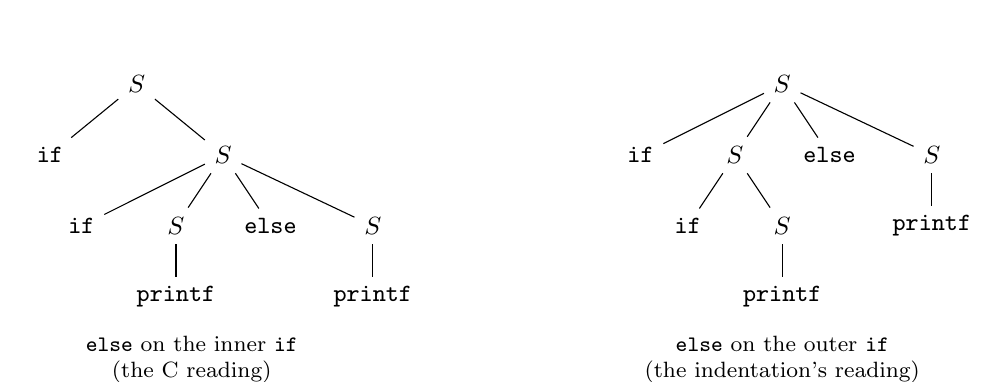
\begin{tikzpicture}[font=\small]
    % ---- else attaches to the inner if
    \begin{scope}
      \node (a) at (1.6, 2.7) {$S$};
      \node (b) at (0.5, 1.8) {\texttt{if}};
      \node (c) at (2.7, 1.8) {$S$};
      \node (d) at (0.9, 0.9) {\texttt{if}};
      \node (e) at (2.1, 0.9) {$S$};
      \node (f) at (3.3, 0.9) {\texttt{else}};
      \node (g) at (4.6, 0.9) {$S$};
      \node (h) at (2.1, 0.0) {\texttt{printf}};
      \node (i) at (4.6, 0.0) {\texttt{printf}};
      \foreach \u/\v in {a/b,a/c,c/d,c/e,c/f,c/g,e/h,g/i} { \draw (\u) -- (\v); }
      \node[font=\footnotesize, align=center] at (2.3,-0.8)
        {\texttt{else} on the inner \texttt{if}\\ (the C reading)};
    \end{scope}
    % ---- else attaches to the outer if
    \begin{scope}[xshift=7.6cm]
      \node (A) at (2.2, 2.7) {$S$};
      \node (B) at (0.4, 1.8) {\texttt{if}};
      \node (C) at (1.6, 1.8) {$S$};
      \node (D) at (2.8, 1.8) {\texttt{else}};
      \node (E) at (4.1, 1.8) {$S$};
      \node (F) at (1.0, 0.9) {\texttt{if}};
      \node (G) at (2.2, 0.9) {$S$};
      \node (H) at (4.1, 0.9) {\texttt{printf}};
      \node (I) at (2.2, 0.0) {\texttt{printf}};
      \foreach \u/\v in {A/B,A/C,A/D,A/E,C/F,C/G,E/H,G/I} { \draw (\u) -- (\v); }
      \node[font=\footnotesize, align=center] at (2.2,-0.8)
        {\texttt{else} on the outer \texttt{if}\\ (the indentation's reading)};
    \end{scope}
  \end{tikzpicture}
\end{figure}

\begin{problem}[Exercice --- rendre la grammaire non ambiguë]
  Modifier la grammaire pour la rendre non ambiguë.
\end{problem}

\begin{example}[Solution]
  \[
    \begin{aligned}
      S  &\to \texttt{if}\, S       & \qquad IE &\to \texttt{printf} \\
      S  &\to IE                    & \qquad IE &\to \texttt{if}\, IE\ \texttt{else}\, S
    \end{aligned}
  \]
  A new non-terminal $IE$ is introduced and the then-branch of an
  \verb|if|\dots\verb|else| is restricted to it: only $IE$, never $S$, may sit
  between an \verb|if| and its \verb|else|. That is what puts the \verb|else| on
  the inner \verb|if| in the tree below, and it disambiguates the example the
  exercise was set on.
\end{example}

\begin{remark}
  It does \emph{not} disambiguate the grammar in general, and it is worth seeing
  why, because the tempting justification --- that $IE$ is \emph{closed}, i.e.\
  cannot swallow a following \verb|else| --- is false. The rule
  $IE \to \texttt{if}\, IE\ \texttt{else}\, S$ ends in $S$, and $S \to
  \texttt{if}\, S$, so an $IE$ can itself end in an unmatched \verb|if|. The
  shortest witness is
  \[ \texttt{if if printf else if printf else printf} \]
  which still has \textbf{two} arbres de dérivation: the final \verb|else| can
  bind the third \verb|if| (via $S \to \texttt{if}\, S$ with the inner $S$ an $IE$),
  or bind the outermost one (via $S \to IE$ with
  $\texttt{if if printf else if printf}$ derived as the inner $IE$), leaving the
  third \verb|if| dangling. Every shorter mot has a unique tree, which is why
  a single illustrative derivation, like the one drawn below, looks conclusive.
  Closing the construction properly requires the else-branch to be closed too:
  $IE \to \texttt{if}\, IE\ \texttt{else}\, IE$.
\end{remark}

\begin{figure}[h!]
  \centering
  \begin{tikzpicture}[font=\small]
    \node (a) at (1.8, 3.6) {$S$};
    \node (b) at (0.6, 2.7) {\texttt{if}};
    \node (c) at (3.0, 2.7) {$S$};
    \node (d) at (3.0, 1.8) {$IE$};
    \node (e) at (1.1, 0.9) {\texttt{if}};
    \node (f) at (2.4, 0.9) {$IE$};
    \node (g) at (3.6, 0.9) {\texttt{else}};
    \node (h) at (5.0, 0.9) {$S$};
    \node (i) at (2.4, 0.0) {\texttt{printf}};
    \node (j) at (5.0, 0.0) {$IE$};
    \node (k) at (5.0,-0.9) {\texttt{printf}};
    \foreach \u/\v in {a/b,a/c,c/d,d/e,d/f,d/g,d/h,f/i,h/j,j/k} { \draw (\u) -- (\v); }
  \end{tikzpicture}
\end{figure}

\subsubsection{Gérer la précédence des opérateurs}
The same disease, in its arithmetic form. Take
\[
  S \to \texttt{int}, \qquad S \to S+S, \qquad S \to S*S, \qquad S \to S \hat{\ } S ,
\]
and again the exercise is: modifier la grammaire pour la rendre non ambiguë.

\begin{example}[A first solution, and why it is wrong]
  \[
    S \to E+S, \qquad S \to E*S, \qquad S \to E \hat{\ } S, \qquad E \to \texttt{int} .
  \]
  Forcing the left operand down to a single \verb|int| does remove the
  ambiguity --- every operator now cuts the expression at its first occurrence
  --- but it removes it the wrong way.
  $6 + 5 * 4 \hat{\ } 3 * 2 + 1$ est lu comme
  \[
    6 + \bigl(5 * (4 \hat{\ } (3 * (2 + 1)))\bigr)
    \qquad\text{whereas one would rather want}\qquad
    6 + \bigl(5 * (4 \hat{\ } 3) * 2\bigr) + 1 .
  \]
  All three operators have become right-associative and all three have the same
  precedence, because a single non-terminal $S$ is doing the work of three
  different levels.
\end{example}

\begin{example}[A better solution: stratify by precedence]
  Attribuer une \textbf{précédence} à chaque opérateur, $0$ pour $+$, $1$ pour
  $*$ et $2$ pour $\hat{\ }$. Then give each level its own non-terminal
  $S_{i}$:
  \[
    \begin{aligned}
      S_{0} &\to S_{0} + S_{1}   & S_{1} &\to S_{1} * S_{2}          & S_{2} &\to S_{3} \hat{\ } S_{2} \\
      S_{0} &\to S_{1}           & S_{1} &\to S_{2}                  & S_{2} &\to S_{3} \\
            &                    &       &                          & S_{3} &\to \texttt{int}
    \end{aligned}
  \]
  A level-$i$ expression is a chain of level-$i$ operators whose operands are
  level-$(i{+}1)$ expressions, and the ``escape'' rule $S_{i} \to S_{i+1}$ lets
  a tighter-binding expression be used wherever a looser one is expected. The
  precedence is now structural: $*$ cannot appear at the top of an $S_{0}$
  chain except inside an $S_{1}$.
\end{example}

\begin{remark}[Associativité comes for free]
  Cela gère même l'\textbf{associativité} (\textit{associativity}) droite ou
  gauche --- the knob is which side the recursion is on. With
  \[
    \begin{aligned}
      S_{0} &\to S_{0} + S_{1} & S_{1} &\to S_{1} * S_{2} & S_{2} &\to S_{3} \hat{\ } S_{2} \\
      S_{0} &\to S_{0} - S_{1} & S_{1} &\to S_{1} / S_{2} & S_{2} &\to S_{3} \\
      S_{0} &\to S_{1}         & S_{1} &\to S_{2}         & S_{3} &\to \texttt{int}
    \end{aligned}
  \]
  one gets
  \[
    2 \hat{\ } 3 \hat{\ } 4 \;\Rightarrow\; 2^{(3^{4})} \neq (2^{3})^{4} ,
    \qquad
    1 - 2 - 3 \;\Rightarrow\; (1-2)-3 .
  \]
  $S_{0}$ recurses on the \emph{left}, so $+$ and $-$ are left-associative;
  $S_{2}$ recurses on the \emph{right}, so $\hat{\ }$ is right-associative.
  That is the arithmetic one wants, and it costs one character of grammar.
\end{remark}

\subsection{Reconnaître une grammaire non contextuelle}

\subsubsection{Binarisation}
\begin{definition}[CFG binaire]
  Une CFG est \textbf{binaire} si toutes les règles de production sont de la
  forme
  \[
    N \to \epsilon \union (N \union \Sigma) \union (N \union \Sigma)^{2} ,
  \]
  i.e.\ if every right-hand side is empty, a single symbol, or a pair of
  symbols.
\end{definition}

\begin{theorem}[Binarisation]
  Toute CFG $G$ admet une CFG binaire $G'$ telle que $L(G) = L(G')$.
\end{theorem}

\begin{proofsketch}
  On répète la procédure suivante : si $G$ contient $X \to s_{1} \dots s_{k}$
  (with $k > 2$), on réécrit cette règle en les deux règles $X \to s_{1}F$ et
  $F \to s_{2} \dots s_{k}$ avec $F$ un symbole non-terminal frais. Each step
  decreases the total length of the right-hand sides that are too long, so the
  procedure terminates. \qed
\end{proofsketch}

\begin{remark}
  This is \emph{not} Chomsky normal form: $\epsilon$-productions and unit
  productions $N \to M$ survive binarisation, and the recognition algorithm
  below is written to cope with both. The price of binarisation is that the
  arbres de dérivation of $G'$ are not those of $G$ --- the fresh symbols $F$
  appear as spurious internal nodes, which have to be flattened out again if the
  tree is what one is after.
\end{remark}

\subsubsection{Algorithme de reconnaissance}
\begin{definition}[La relation \textit{match}]
  Étant donné un mot $w = w_{0} \dots w_{n-1}$ et une grammaire binaire $G$, on
  dit que $(\alpha, i, j) \in \mathit{match}$ pour $\alpha$ un symbole de $G$ et
  $0 \leq i \leq j \leq n$ si $\alpha$ peut se dériver en
  $w_{i} \dots w_{j-1}$.
\end{definition}

\begin{notation}
  The triple is written both as $(\alpha,i,j)$ and as $(i,j,\alpha)$; they
  are the same object. The convention throughout is that the span is
  \emph{half-open}: $(i,j)$ covers $w_{i} \dots w_{j-1}$, so a single lexème
  $w_{i}$ has span $(i,i+1)$ and the whole word has span $(0,n)$.
\end{notation}

\begin{definition}[\textit{match} comme plus petit point fixe (\textit{fixpoint})]
  L'ensemble $\mathit{match}$ est le plus petit ensemble qui contient :
  \begin{itemize}
    \item $(i,i,\alpha)$ si $\alpha \to \epsilon \in G$ ;
    \item $(i,i+1,w_{i})$ pour tout $i < n$ ;
    \item $(i,j,\alpha)$ si $\alpha \to \beta \in G$ et
      $(i,j,\beta) \in \mathit{match}$ ;
    \item $(i,j,\alpha)$ si $\alpha \to \beta\gamma \in G$,
      $(i,k,\beta) \in \mathit{match}$ et $(k,j,\gamma) \in \mathit{match}$.
  \end{itemize}
\end{definition}

\begin{theorem}
  On a $w \in L(G)$ si et seulement si $(S,0,n) \in \mathit{match}$.
\end{theorem}

\subsubsection{Calcul de \textit{match}}
The definition is a point fixe; the algorithm is the obvious worklist that
saturates it. Initialiser $\mathit{match}$ avec
\begin{itemize}
  \item $(i,i,\alpha)$ si $\alpha \to \epsilon \in G$ ;
  \item $(i,i+1,w_{i})$ pour tout $i < n$.
\end{itemize}
Ensuite on traite les éléments $(i,j,\alpha)$ de $\mathit{match}$ \emph{un par
un} en appliquant les règles suivantes :
\begin{itemize}
  \item si $\beta \to \alpha \in G$ on ajoute $(i,j,\beta)$ ;
  \item si $\beta \to \alpha\gamma \in G$, pour $k \geq j$ t.q.\
    $(j,k,\gamma) \in \mathit{match}$ on ajoute $(i,k,\beta)$ ;
  \item si $\beta \to \gamma\alpha \in G$, pour $k \leq i$ t.q.\
    $(k,i,\gamma) \in \mathit{match}$ on ajoute $(k,j,\beta)$.
\end{itemize}

Pour $(i,j)$ donnés, chaque production est considérée au plus $2n$ fois.
Hence
\[
  \boxed{\text{Complexity } O(n^{3} \times |G|)} .
\]

\begin{remark}[Which algorithm this is]
  This is the \textbf{CYK} algorithm (Cocke--Younger--Kasami), in agenda form.
  The textbook presentation fills a triangular table indexed by $(i,j)$ in order
  of increasing span length and demands Chomsky normal form; the presentation
  here computes exactly the same relation $\mathit{match}$ as a least point fixe
  driven by a worklist, and asks only for binarisation. The two shapes of the
  last rule --- extend to the right with $\beta \to \alpha\gamma$, extend to the
  left with $\beta \to \gamma\alpha$ --- are what replaces the ordered sweep:
  since items are not produced in order of length, a new item must be offered
  both as a left part and as a right part of every binary production. The factor
  $2n$ in the count is precisely those two directions times the $n$ possible
  values of $k$.
\end{remark}

\subsubsection{Retrouver l'arbre de dérivation}
Recognition is not analyse syntaxique: $(S,0,n) \in \mathit{match}$ answers yes
or no and returns no tree. One recovers the tree by carrying a witness alongside
every item. On ajoute à $\mathit{match}$ un \textbf{tableau} $D$ avec
\begin{itemize}
  \item $D[i,i,\alpha] = \alpha$ si $\alpha \to \epsilon \in G$ ;
  \item $D[i,i+1,w_{i}] = w_{i}$ pour tout $i < n$.
\end{itemize}
Ensuite pour les éléments $(i,j,\alpha) \to t$ de $\mathit{match}$, on a :
\begin{itemize}
  \item si $\beta \to \alpha \in G$ alors $D[i,j,\beta] = \beta(t)$ ;
  \item si $\beta \to \alpha\gamma \in G$, pour $k \geq j$ t.q.\
    $D[j,k,\gamma] = t' \neq \emptyset$ alors $D[i,k,\beta] = \beta(t,t')$ ;
  \item si $\beta \to \gamma\alpha \in G$, pour $k \leq i$ t.q.\
    $D[k,i,\gamma] = t' \neq \emptyset$ alors $D[k,j,\beta] = \beta(t',t)$.
\end{itemize}
Pour $(i,j)$ donnés, chaque production est considérée au plus $2n$ fois. The
complexity is therefore unchanged: $O(n^{3} \times |G|)$.

\begin{remark}
  In the unit bullet, $D[i,j,\beta] = \beta(t)$ is a $\beta$-node with the
  $\alpha$-subtree $t$ as its only child. The node is labelled $\beta$ because
  the item being filled is the one for $\beta$, exactly as in the two binary
  bullets; $\alpha$ labels only the root of its child.
\end{remark}

\begin{remark}
  $D$ stores \emph{one} tree per cell, so it returns one parse of an ambiguous
  word and silently drops the others. Storing the set of all trees would cost
  exponential space; what is stored instead, in a real implementation, is the
  set of backward \emph{pointeurs} per cell --- the shared packed parse forest
  --- which stays cubic.
\end{remark}

\subsection{Faisons tourner l'algorithme}
Here the algorithm is run by hand on the grammar below, in its
\textbf{non-binarised} version: the right-hand sides are matched whole against
consecutive spans rather than two symbols at a time. Nothing else changes ---
the items are still triples $(i,j,\alpha)$ and the closure rules are still the
same --- but the trace stays readable, because the rule
$S \to \texttt{let var} = S\ \texttt{in}\ S$ is applied in one step instead of
five.

\[
  \begin{aligned}
    S &\to \texttt{let var} = S\ \texttt{in}\ S & \qquad P &\to T   & \qquad T &\to \texttt{var} \\
    S &\to P                                    & \qquad P &\to T*P & \qquad T &\to \texttt{int} \\
    S &\to P+S                                  &          &       &          &
  \end{aligned}
\]

\noindent The input is \verb|1+let x = 2 in x*3+4|, which the lexeur has already
turned into twelve lexèmes; $n = 12$ and the boundaries run from $0$ to $12$.

\begin{center}
  \begin{tabular}{c|c|c|c|c|c|c|c|c|c|c|c}
    \toprule
    \texttt{1} & \texttt{+} & \textit{let} & \texttt{x} & \texttt{=} & \texttt{2}
    & \textit{in} & \texttt{x} & \texttt{*} & \texttt{3} & \texttt{+} & \texttt{4} \\
    0 & 1 & 2 & 3 & 4 & 5 & 6 & 7 & 8 & 9 & 10 & 11 \\
    \bottomrule
  \end{tabular}
\end{center}

The trace works from the right end of the input towards the left. At each step
the items that can no longer be useful are dropped from the display, which is
why the list does not simply grow.

\begin{center}
  \begin{tabular}{r l l}
    \toprule
    & Item derived & Justification \\
    \midrule
    1 & $(11,12,T)$, $(11,12,P)$, $(11,12,S)$
      & $\texttt{4} \leftarrow T \leftarrow P \leftarrow S$ \\
    2 & $(9,10,T)$, $(9,10,P)$
      & $\texttt{3} \leftarrow T \leftarrow P$ \\
    3 & $(7,8,T)$
      & $\texttt{x} \leftarrow T$ (rule $T \to \texttt{var}$) \\
    4 & $(7,10,P)$
      & $P \to T*P$ on $(7,8,T)$, $(8,9,*)$, $(9,10,P)$ \\
    5 & $(7,12,S)$
      & $S \to P+S$ on $(7,10,P)$, $(10,11,+)$, $(11,12,S)$ \\
    6 & $(5,6,S)$
      & $\texttt{2} \leftarrow T \leftarrow P \leftarrow S$ \\
    7 & $(2,12,S)$
      & $S \to \texttt{let var} = S\ \texttt{in}\ S$ on $(5,6,S)$ and $(7,12,S)$ \\
    8 & $(0,1,P)$
      & $\texttt{1} \leftarrow T \leftarrow P$ \\
    9 & $(0,12,S)$
      & $S \to P+S$ on $(0,1,P)$, $(1,2,+)$, $(2,12,S)$ \\
    \bottomrule
  \end{tabular}
\end{center}

\noindent $(S,0,12) \in \mathit{match}$ with $n = 12$, so the word is accepté.

\begin{figure}[h!]
  \centering
  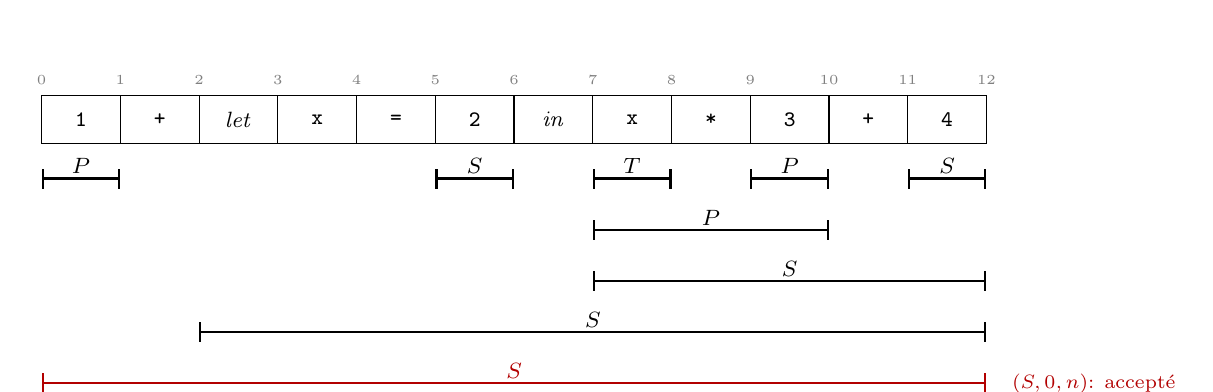
\begin{tikzpicture}[font=\footnotesize, x=1.0cm]
    % token cells
    \foreach \i/\t in {0/{\texttt{1}},1/{\texttt{+}},2/{\textit{let}},3/{\texttt{x}},
                       4/{\texttt{=}},5/{\texttt{2}},6/{\textit{in}},7/{\texttt{x}},
                       8/{\texttt{*}},9/{\texttt{3}},10/{\texttt{+}},11/{\texttt{4}}} {
      \draw (\i,0) rectangle (\i+1,0.6);
      \node at (\i+0.5,0.3) {\t};
    }
    % boundary numbers
    \foreach \i in {0,...,12} {
      \node[anchor=south, font=\tiny, gray] at (\i,0.62) {\i};
    }
    % span bars
    \tikzset{span/.style={|-|, thick}}
    \foreach \a/\b/\lab/\y in {%
      0/1/{$P$}/-0.45, 5/6/{$S$}/-0.45, 7/8/{$T$}/-0.45,
      9/10/{$P$}/-0.45, 11/12/{$S$}/-0.45} {
      \draw[span] (\a,\y) -- (\b,\y);
      \node[anchor=south, inner sep=1.5pt] at ({(\a+\b)/2},\y) {\lab};
    }
    \draw[span] (7,-1.1) -- (10,-1.1);
    \node[anchor=south, inner sep=1.5pt] at (8.5,-1.1) {$P$};
    \draw[span] (7,-1.75) -- (12,-1.75);
    \node[anchor=south, inner sep=1.5pt] at (9.5,-1.75) {$S$};
    \draw[span] (2,-2.4) -- (12,-2.4);
    \node[anchor=south, inner sep=1.5pt] at (7,-2.4) {$S$};
    \draw[span, red!70!black] (0,-3.05) -- (12,-3.05);
    \node[anchor=south, inner sep=1.5pt, red!70!black] at (6,-3.05) {$S$};
    \node[anchor=west, font=\scriptsize, red!70!black] at (12.2,-3.05)
      {$(S,0,n)$: accepté};
  \end{tikzpicture}
\end{figure}

\begin{remark}[Checking the trace]
  Two checks apply to any trace. First, a span always has $i \leq j$: the
  lexème \verb|3| sits at index $9$, so step 2 yields $(9,10,T)$ alongside
  $(9,10,P)$. Second, every justification names productions of the grammar:
  the last step is $S \to P + S$ applied to $(0,1,P)$, $(1,2,+)$ and
  $(2,12,S)$.
\end{remark}

\begin{remark}[Why is this grammar not ambiguous?]
  The answer is that the three non-terminaux are \emph{stratified} exactly as
  in the precedence construction above: $T$ derives a single lexème, $P$
  derives a $*$-chain of $T$s, and $S$ derives a $+$-chain of $P$s or a
  \verb|let|-expression. So for any given span at most one production can apply:
  a span containing a top-level $+$ is not a $P$, and no $P$ or $T$ can start
  with \verb|let|. Where a rule mentions the same non-terminal twice --- $T*P$,
  $P+S$ --- the recursion is on the right only, so the cut is forced at the
  \emph{first} operator of the chain and there is nothing left to choose. Both
  operators therefore come out right-associative.
\end{remark}

\subsection{Utilisation en pratique}
La reconnaissance de mots par CFG est en $O(n^{3} \times |G|)$, cela peut
sembler raisonnable mais :

\begin{itemize}
  \item les fichiers de code contiennent parfois plusieurs milliers de lignes
    (et plus si on compte les entêtes inclus) ;
  \item cela peut faire de l'ordre de la centaine de milliers voire du million
    de symboles ;
  \item un processeur des années 70 faisait $\sim 10^{6}$ opérations par
    seconde $\Rightarrow$ il aurait fallu $30\,000$ ans pour faire $10^{18}$
    opérations ;
  \item un processeur moderne fait $\sim 10^{9}$ opérations par seconde
    $\Rightarrow$ il faut $32$ ans pour faire $10^{18}$ opérations.
\end{itemize}

\begin{remark}
  $10^{18}$ is $n^{3}$ for $n = 10^{6}$, so the two lines are the same
  computation on the same file. The point is the exponent, not the constant:
  four decades of hardware progress moved a cubic algorithm from
  ``geologically impossible'' to ``merely impossible''. Hence les langages
  utilisent souvent des grammaires avec \textbf{test linéaire}
  (\textit{linear test}).
\end{remark}

\begin{figure}[h!]
  \centering
  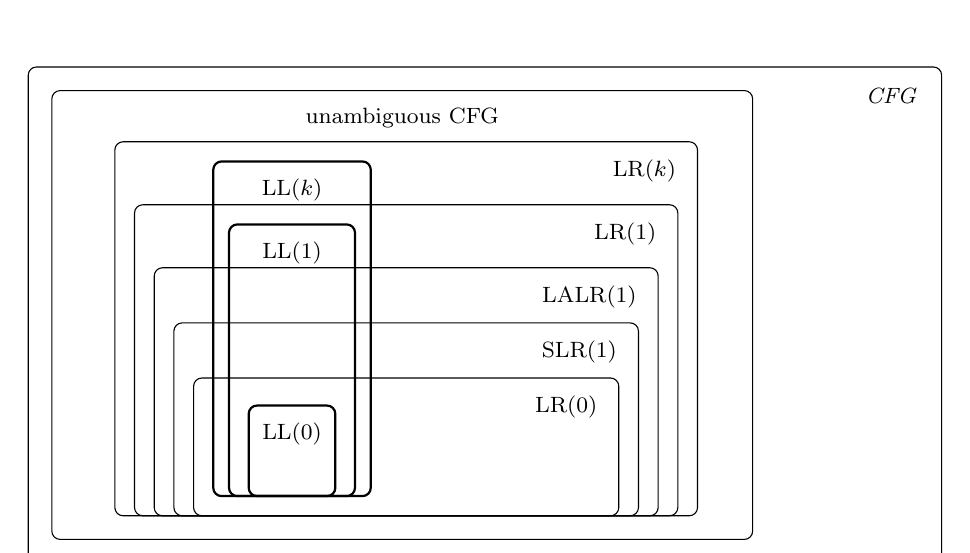
\begin{tikzpicture}[font=\footnotesize]
    \tikzset{cls/.style={draw, rounded corners=3pt}}
    % outermost : CFG
    \draw[cls] (0,0) rectangle (11.6,6.3);
    \node[anchor=north east, font=\footnotesize\itshape] at (11.4,6.15) {CFG};
    % unambiguous CFG
    \draw[cls] (0.3,0.3) rectangle (9.2,6.0);
    \node[anchor=north] at (4.75,5.9) {unambiguous CFG};
    % LR chain
    \draw[cls] (1.1,0.6) rectangle (8.5,5.35);
    \node[anchor=north east] at (8.35,5.25) {LR($k$)};
    \draw[cls] (1.35,0.6) rectangle (8.25,4.55);
    \node[anchor=north east] at (8.1,4.45) {LR($1$)};
    \draw[cls] (1.6,0.6) rectangle (8.0,3.75);
    \node[anchor=north east] at (7.85,3.65) {LALR($1$)};
    \draw[cls] (1.85,0.6) rectangle (7.75,3.05);
    \node[anchor=north east] at (7.6,2.95) {SLR($1$)};
    \draw[cls] (2.1,0.6) rectangle (7.5,2.35);
    \node[anchor=north east] at (7.35,2.25) {LR($0$)};
    % LL chain, crossing the LR boxes on the left
    \draw[cls, thick] (2.35,0.85) rectangle (4.35,5.1);
    \node[anchor=north] at (3.35,5.0) {LL($k$)};
    \draw[cls, thick] (2.55,0.85) rectangle (4.15,4.3);
    \node[anchor=north] at (3.35,4.2) {LL($1$)};
    \draw[cls, thick] (2.8,0.85) rectangle (3.9,2.0);
    \node[anchor=north] at (3.35,1.9) {LL($0$)};
  \end{tikzpicture}
\end{figure}

\noindent Read the picture as inclusions of \emph{grammar} classes, not of
languages: $\text{LR}(0) \subset \text{SLR}(1) \subset \text{LALR}(1) \subset
\text{LR}(1) \subset \text{LR}(k)$, all of them non-ambiguës, and the LL boxes
cut across them --- $\text{LL}(0) \subset \text{LL}(1) \subset \text{LL}(k)$
with each $\text{LL}(i)$ inside the corresponding $\text{LR}(i)$. The
\textit{lookahead} $k$ is the number of lexèmes the parser is allowed to peek at,
and the classes with $k = 1$ are the ones for which parser generators exist.

\subsection{Analyse syntaxique descendante}

Comment reconnaître \emph{rapidement} une telle grammaire ? Take the stratified
expression grammar, reduced to two operators:
\[
  \begin{aligned}
    S_{0} &\to S_{1} + S_{0} & \qquad S_{1} &\to S_{2} * S_{1} & \qquad S_{2} &\to \texttt{int} \\
    S_{0} &\to S_{1}         & \qquad S_{1} &\to S_{2}         &              &
  \end{aligned}
\]

\begin{example}[Recursive descent by hand]
  With two primitives on the lexème stream --- \verb|peek()| donne le prochain
  symbole à lire sans le consommer, \verb|eat()| donne et consomme le prochain
  symbole --- one function per non-terminal suffices.

\begin{lstlisting}[language=Python]
peek() # donne le prochain symbole a lire sans le consommer
eat()  # donne et consomme le prochain symbole

def s0():                def s1():                def s2():
  a = s1()                 a = s2()                 a = peek()
  if peek() != '+':        if peek() != '*':        assert(a == 'int')
    return a                 return a               eat()
  eat()                    eat()                    return a
  return (a,'+',s0())      return (a,'*',s1())
\end{lstlisting}

  Each function returns the subtree it has just recognised; the tuple
  \verb|(a,'+',s0())| \emph{is} the node of the arbre de dérivation. Note that
  the recursive call sits in the returned tuple, i.e.\ at the right of the node,
  matching the right recursion of $S_{0} \to S_{1} + S_{0}$.
\end{example}

\begin{remark}
  This is why the method is called \textbf{descendante} (\textit{top-down}): the
  parser starts at $S$ and descends, choosing a production before it has seen
  what it derives. The CYK algorithm of the previous section is the opposite ---
  bottom-up, combining items already recognised. Analyse syntaxique descendante
  is linear and fits in twelve lines; the price is that the choice of production
  has to be decidable from the next lexème alone, which is exactly the LL(1)
  condition.
\end{remark}

\subsubsection{Pourquoi cela marche et peut-on généraliser ?}
Commençons par réécrire la grammaire, so that the choice is never between two
productions that begin the same way --- \textbf{factorisation à gauche}
(\textit{left factoring}):
\[
  \begin{aligned}
    S_{0} &\to S_{1}F_{0} & \qquad S_{1} &\to S_{2}F_{1} & \qquad S_{2} &\to \texttt{int} \\
    F_{0} &\to +S_{0}     & \qquad F_{1} &\to *S_{1}     &              & \\
    F_{0} &\to \epsilon   & \qquad F_{1} &\to \epsilon   &              &
  \end{aligned}
\]
The common prefix $S_{1}$ of the two $S_{0}$-rules has been pulled out, and what
was the choice between $S_{1} + S_{0}$ and $S_{1}$ has become the choice, inside
$F_{0}$, between consuming a $+$ and producing nothing. The rewritten grammar is
a transcription of the code: the \verb|if peek() != '+': return a| is exactly
$F_{0} \to \epsilon$.

\begin{definition}[Les trois ensembles]
  \leavevmode
  \begin{itemize}
    \item \textit{Null}: the set of non-terminaux $X$ such that
      $X \Rightarrow \epsilon$;
    \item $\mathit{Suivant}(X)$ (\textit{follow}) : les terminaux qui peuvent
      suivre $X$ ;
    \item $\mathit{Premier}(X)$ (\textit{first}) : les terminaux qui peuvent
      commencer un mot dérivé de $X$.
  \end{itemize}
\end{definition}

\begin{remark}
  \textit{Null} is a set of \emph{non-terminaux}. A terminal derives only
  itself, so no \emph{terminal} $X$ satisfies $X \Rightarrow \epsilon$, and a
  \textit{Null} made of terminaux would always be empty. The computed value
  $\{F_{0},F_{1}\}$ below is indeed a set of non-terminaux.
\end{remark}

\begin{example}[The three sets on the factored grammar]
  \[
    \mathit{Null} = \{F_{0}, F_{1}\}
  \]
  \[
    \begin{aligned}
      \mathit{Premier}(S_{i}) &= \{\texttt{int}\} & \qquad
      \mathit{Suivant}(S_{0}) = \mathit{Suivant}(F_{0}) &= \{\} \\
      \mathit{Premier}(F_{0}) &= \{+\}            & \qquad
      \mathit{Suivant}(S_{1}) = \mathit{Suivant}(F_{1}) &= \{+\} \\
      \mathit{Premier}(F_{1}) &= \{*\}            & \qquad
      \mathit{Suivant}(S_{2}) &= \{*, +\}
    \end{aligned}
  \]
  Every $S_{i}$ begins with \verb|int| because every chain bottoms out at
  $S_{2} \to \texttt{int}$. $\mathit{Suivant}(S_{0})$ is empty because $S_{0}$
  is the symbole de départ and nothing follows the whole input.
  $\mathit{Suivant}(S_{2}) = \{*,+\}$ collects $\mathit{Premier}(F_{1}) = \{*\}$
  from $S_{1} \to S_{2}F_{1}$ and, because $F_{1}$ is nullable,
  $\mathit{Suivant}(S_{1}) = \{+\}$ as well.
\end{example}

\begin{definition}[Grammaire LL(1)]
  \textbf{Grammaire LL(1)} : grammaire qui ne contient pas $X \to \alpha$ et
  $X \to \beta$ ($\alpha \neq \beta$) telles que (any one of the following is
  enough) :
  \begin{itemize}
    \item $\alpha$ et $\beta$ dérivent toutes deux $\epsilon$ ;
    \item $\mathit{Premier}(\alpha) \intersect \mathit{Premier}(\beta) \neq \emptyset$ ;
    \item $\alpha$ dérive $\epsilon$ et
      $\mathit{Premier}(\beta) \intersect \mathit{Suivant}(X) \neq \emptyset$.
  \end{itemize}
\end{definition}

\noindent $\Rightarrow$ définition alternative de LL(1) : \textbf{le prochain
symbole détermine la production à utiliser}. Each of the three clauses is one
way for two productions of the same $X$ to be indistinguishable on one lexème
of lookahead --- both empty,
both able to start with the same terminal, or one empty and the other able to
start with something that could equally well have been the continuation after
$X$.\\

The factored grammar above violates none of the three, so it is
\textbf{LL(1)} --- and that is the theorem behind the twelve lines of code: for
an LL(1) grammar the recursive-descent parser is well defined, deterministic,
and runs in time linear in the number of lexèmes.

\subsubsection{Exercice --- un analyseur syntaxique descendant pour la grammaire \texttt{let}}
\begin{problem}
  Comprendre pourquoi cette grammaire n'est pas LL(1) puis la modifier pour la
  rendre LL(1) et enfin écrire un analyseur syntaxique descendant.
  \[
    \begin{aligned}
      S &\to \texttt{let var} = S\ \texttt{in}\ S & \qquad P &\to T   & \qquad T &\to \texttt{var} \\
      S &\to P                                    & \qquad P &\to T*P & \qquad T &\to \texttt{int} \\
      S &\to P+S                                  &          &       &          &
    \end{aligned}
  \]
  Terminaux : \verb|var|, \verb|int|, \verb|+|, \verb|*|, \verb|let|, \verb|=|,
  \verb|in|.
\end{problem}

\begin{example}[Worked answer]
  What follows applies the method of the previous subsection.

  \medskip
  \textbf{Why it fails.} $\mathit{Premier}(P) = \mathit{Premier}(T) =
  \{\texttt{var}, \texttt{int}\}$, so the two productions $S \to P$ and
  $S \to P+S$ have intersecting $\mathit{Premier}$ sets and the second clause of
  the definition fires: on seeing \verb|var| the parser cannot tell which to
  choose. The pair $P \to T$ and $P \to T*P$ fails for the same reason. The
  \verb|let| production is fine --- it is the only one beginning with
  \verb|let|.

  \medskip
  \textbf{The fix.} Left-factor both offending pairs, exactly as $S_{0}$ was
  factored into $S_{0} \to S_{1}F_{0}$:
  \[
    \begin{aligned}
      S &\to \texttt{let var} = S\ \texttt{in}\ S & \qquad P &\to T G     & \qquad T &\to \texttt{var} \\
      S &\to P F                                  & \qquad G &\to *P      & \qquad T &\to \texttt{int} \\
      F &\to +S                                   & \qquad G &\to \epsilon &         & \\
      F &\to \epsilon                             &          &            &          &
    \end{aligned}
  \]
  Now $\mathit{Premier}(\texttt{let} \dots) = \{\texttt{let}\}$ is disjoint from
  $\mathit{Premier}(PF) = \{\texttt{var},\texttt{int}\}$; $F$ and $G$ each offer
  a production starting with a distinct operator against an
  $\epsilon$-production, and $+ \notin \mathit{Suivant}(F)$,
  $* \notin \mathit{Suivant}(G)$, so the third clause does not fire either.

  \medskip
  \textbf{The parser.}
\begin{lstlisting}[language=Python]
def s():
  if peek() == 'let':
    eat()                       # let
    v = eat()                   # var
    eat()                       # =
    e1 = s()
    eat()                       # in
    return ('let', v, e1, s())
  a = p()
  if peek() != '+':             # F -> epsilon
    return a
  eat()
  return (a,'+',s())            # F -> + S

def p():
  a = t()
  if peek() != '*':             # G -> epsilon
    return a
  eat()
  return (a,'*',p())            # G -> * P

def t():
  a = peek()
  assert(a == 'var' or a == 'int')
  eat()
  return a
\end{lstlisting}
  One function per non-terminal of the \emph{unfactored} grammar; the factored
  $F$ and $G$ appear as the trailing \verb|if| inside \verb|s()| and \verb|p()|
  rather than as functions of their own, which is the usual way the
  factorisation is written back into code.
\end{example}

\subsection{De nombreuses classes\dots}
Il existe d'autres classes intéressantes, considérons maintenant les CFG où
toutes les productions sont de la forme
\[
  N \to \Sigma \times N \union \epsilon ,
\]
that is, every right-hand side is either a terminal followed by a single
non-terminal, or empty.

\begin{theorem}
  These are exactly the \textbf{langages réguliers} (\textit{regular
  languages}).
\end{theorem}

\begin{remark}
  Such grammars are the \textbf{right-linear} ones, and the correspondence with
  automates finis is immediate: read each non-terminal as an état, each rule
  $N \to cM$ as a transition $N \xrightarrow{\,c\,} M$, and each rule
  $N \to \epsilon$ as ``$N$ is accepting''. The symbole de départ is the état
  initial. Nothing is lost and nothing is added, which is why the next chapter
  can speak of automates and of grammars interchangeably.
\end{remark}

\begin{figure}[h!]
  \centering
  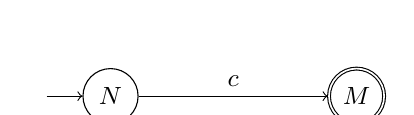
\begin{tikzpicture}[font=\small, node distance=2.4cm,
                      every state/.style={minimum size=7mm, inner sep=1pt}]
    \node[state, initial, initial text={}] (N) {$N$};
    \node[state, accepting, right=of N] (M) {$M$};
    \path[->] (N) edge node[above] {$c$} (M);
  \end{tikzpicture}
\end{figure}

\noindent The rules $N \to cM$ and $M \to \epsilon$, read as an automate.

\begin{conclusion}
  Four thresholds structure the chapter, and each one is a restriction paid for
  with an algorithm. General grammaires formelles: problème de l'appartenance
  indécidable. Restrict the left-hand side to a single non-terminal and one gets
  the grammaires non contextuelles, where the problème de l'appartenance is
  decided in $O(n^{3} \times |G|)$ by saturating the relation $\mathit{match}$
  --- CYK --- after binarising the productions. Cubic is still hopeless on a
  file of a million lexèmes, so restrict further to the grammars whose next
  production is determined by the next lexème: LL(1), tested with
  \textit{Null}, $\mathit{Premier}$ and $\mathit{Suivant}$, parsed in linear
  time by one recursive function per non-terminal. Restrict once more, to
  right-linear productions, and one has fallen out of analyse syntaxique
  altogether into the langages réguliers and automates finis --- which is where
  the lexeur lives, and where the next chapter begins.\\

  The recurring technique, across all four levels, is \emph{rewriting the
  grammar rather than the parser}: stratify by precedence to fix associativité,
  introduce a closed non-terminal to fix the dangling \verb|else|, binarise to
  fit CYK, left-factor to fit LL(1). The language recognised never changes; only
  the shape of the trees, and the algorithm that can afford to build them.
\end{conclusion}

\section{Langages réguliers et analyse lexicale}
The chapter on analyse syntaxique ended by narrowing grammaires non
contextuelles until nothing much was left: les CFG où toutes les productions
sont de la forme
\[
  N \;\to\; \Sigma \times N \;\cup\; \epsilon ,
\]
that is, a terminal followed by a single non-terminal, or nothing at all. That
class has a name --- \emph{les langages réguliers}. This chapter is that class
seen from three sides at once: as expressions régulières, which a human
writes; as automates, which a machine runs; and as the front end of the
compilateur which uses both, the \textit{lexeur}. It closes on writing a lexeur
from scratch.

\subsection{Langages réguliers}
\begin{definition}[Diverses définitions]
  On peut définir les langages réguliers de diverses manières :
  \begin{itemize}
    \item via les \textbf{opérations rationnelles} (\textit{rational
      operations}) ;
    \item par les expressions régulières ;
    \item par les automates ;
    \item comme image inverse de \textbf{monoïdes finis} (\textit{finite
      monoids}) ;
    \item par la \textbf{logique} (\textit{logic}) ;
    \item etc.
  \end{itemize}
\end{definition}

\begin{remark}
  The list is not padding. A class of languages with one definition is a
  curiosity; a class with five unrelated-looking definitions that all pick out
  the same sets is a robust object, and each definition is good at a different
  job. The right-linear grammars above are a sixth entry, reached from the side
  of analyse syntaxique. Only two of them are developed here, and they are
  chosen for opposite reasons: expressions because they are what one writes,
  automates because they are what one runs.
\end{remark}

\subsection{Expressions régulières}
\subsubsection{Syntaxe}
\begin{definition}[Expressions régulières, inductivement]
  On définit inductivement les expressions régulières :
  \[
    \begin{array}{r@{\;}l@{\qquad}l}
      r \mathrel{\Coloneqq} & \emptyset      & \text{langage vide --- the empty language} \\
                            & \epsilon       & \text{mot vide --- the empty word} \\
                            & c              & c \text{ un caractère --- a character} \\
                            & [c_1 - c_2]    & \text{une classe de caractères --- a character class} \\
                            & r \mid r       & \text{union} \\
                            & r\,r           & \text{concaténation} \\
                            & r{*}           & \text{répétition (zéro ou plus)} \\
                            & r{+}           & \text{répétition (au moins une fois)}
    \end{array}
  \]
\end{definition}

Eight cases, of which the first four are atoms and the last four are
constructors. Note that this is a definition of \emph{syntax} only: at this
stage $r{*}$ is a tree node with one child, nothing more. What it denotes comes
next, and is a separate definition.

\begin{remark}
  $\emptyset$ and $\epsilon$ are not the same expression and not the same
  language. $\emptyset$ denotes the language with no words at all;
  $\epsilon$ denotes the language whose single word is the word of length zero.
  Concatenating anything with $\emptyset$ gives $\emptyset$; concatenating
  anything with $\epsilon$ changes nothing. The distinction matters as soon as
  one writes a lexeur rule that can match nothing.
\end{remark}

\subsubsection{Le langage associé}
\begin{definition}[Langage associé]
  On peut aussi définir le \textbf{langage associé} (\textit{associated
  language}) :
  \[
    \begin{array}{r@{\quad}l}
      \text{Expression } r & \text{Langage } L(r) \\[2pt]
      \emptyset    & \emptyset \\
      \epsilon     & \{\epsilon\} \\
      c            & \{c\} \\
      {}[c_1 - c_2]  & \{ c \mid c_1 \le c \le c_2 \} \\
      r_a \mid r_b & L(r_a) \union L(r_b) \\
      r_a r_b      & \{ w_a w_b \mid w_a \in L(r_a),\, w_b \in L(r_b) \} \\
      r{*}         & \{ w_1 \ldots w_k \mid k \ge 0 \wedge \forall i,\, w_i \in L(r) \} \\
      r{+}         & \{ w_1 \ldots w_k \mid k \ge 1 \wedge \forall i,\, w_i \in L(r) \}
    \end{array}
  \]
\end{definition}

The whole table is one structural recursion: the language of a compound
expression is built out of the languages of its parts, so $L$ is total and
unambiguous on the syntax above.

\begin{remark}
  The star and the plus differ in exactly one character of the definition,
  $k \ge 0$ against $k \ge 1$, so $r{+}$ is redundant: $L(r\,r{*}) = L(r{+})$.
  It is kept because it is the case one actually writes --- an integer literal
  is $[0-9]{+}$, never $[0-9][0-9]{*}$ --- and an implementation that omits
  the constructor simply builds it, writing \texttt{Concat(digit, Star(digit))}
  for \texttt{digits}, as in the examples below.
\end{remark}

\begin{remark}
  The character class $[c_1 - c_2]$ is defined by the \emph{order} on
  characters, $c_1 \le c \le c_2$: it is a range in the character encoding, not
  an arbitrary set. That is why \texttt{[a-z]} and \texttt{[A-Z]} have to be
  written as two classes joined by a union --- in ASCII they are not contiguous.
\end{remark}

\subsubsection{Des exemples}
The examples are given not as chaînes de caractères in concrete syntax but as
constructor calls: an expression is a value of an algebraic data type with one
constructor per line of the grammar.

\begin{lstlisting}[language=Python]
digit = CharRange('0','9') # one digit
digits = Concat(digit, Star(digit))
letter = Union(CharRange('a','z'),CharRange('A','Z'))
let_tok = Concat(Char('l'), Concat(Char('e'),Char('t')))
in_tok = Concat(CharRange('i','i'),CharRange('n','n'))
opp = Char('+')
opf = Char('*')
opm = Char('-')
ope = Char('=')
ident = Concat(letter,Star(Union(digit,letter)))
space = Union(Char(' '),Char('\t'))
\end{lstlisting}

These are the very definitions that the lexeur written at the end of this
chapter starts from. Two details of the encoding are worth
reading. \texttt{let\_tok} shows that concatenation is binary, so a three-letter
keyword is a nest of two \texttt{Concat}s; the surface syntax \texttt{let} hides
an association choice that the data type must make explicit. And
\texttt{in\_tok} uses \texttt{CharRange('i','i')} where \texttt{Char('i')} would
do --- a degenerate class of one character, harmless because $c \le c \le c$.

\begin{remark}
  The constructor set is \texttt{Char}, \texttt{CharRange}, \texttt{Union},
  \texttt{Concat}, \texttt{Star}: five of the eight cases of the grammar. There
  is no constructor for $\emptyset$, none for $\epsilon$ and none for $r{+}$, so
  an implementation of the lexeur only has to handle five cases --- with $r{+}$
  spelled \texttt{Concat(r, Star(r))} as in \texttt{digits}.
\end{remark}

\subsection{Les reconnaître}
Knowing what $L(r)$ \emph{is} does not say how to test membership. A
recogniser can work directly on the syntax tree, by mutual recursion over a
fixed word.

\begin{definition}[La fonction match]
  Étant donné un mot $w_0 \ldots w_{n-1}$ fixé on définit
  \[
    \operatorname{match}(R, i) \;=\; \{\, j \mid w_i \ldots w_{j-1} \in L(R) \,\}
  \]
  --- the set of positions at which a factor of $w$ starting at $i$ and matched
  by $R$ may end. On a alors :
  \[
    \begin{array}{r@{\;}c@{\;}l}
      \operatorname{match}(\epsilon, i)      &=& \{i\} \\[2pt]
      \operatorname{match}(c, i)             &=& \{ i+1 \mid \text{si } w_i = c \} \\[2pt]
      \operatorname{match}([c_1, c_2], i)    &=& \{ i+1 \mid \text{si } w_i \in [c_1, c_2] \} \\[2pt]
      \operatorname{match}(R_a \mid R_b, i)  &=& \operatorname{match}(R_a, i) \union \operatorname{match}(R_b, i) \\[2pt]
      \operatorname{match}(R_a / R_b, i)     &=& \bigcup_{j \in \operatorname{match}(R_a, i)} \operatorname{match}(R_b, j) \\[2pt]
      \operatorname{match}(R{*}, i)          &=& \text{point fixe}_X \Big( \{i\} \cup_{j \in X} \operatorname{match}(R, j) \Big)
    \end{array}
  \]
\end{definition}

\begin{notation}
  The fifth line is the concatenation case: it writes $R_a / R_b$ where the
  grammar writes $R_a R_b$, the slash standing in for the invisible
  concatenation operator. One may also write $\mathit{matches}(R, w, j)$ with
  the word passed explicitly; since $w$ is fixed throughout, it is the same
  function as $\operatorname{match}(R, j)$. Note also that the word is indexed
  here from $0$, as $w_0 \ldots w_{n-1}$, whereas the automate and the lexeur
  below index it from $1$, as $w_1 \ldots w_n$. Neither convention is wrong;
  only mixing them inside one implementation is.
\end{notation}

The shape of these equations is what makes them implementable. Every case
returns a \emph{set} of end positions, not a yes/no answer, because an
expression régulière can match several prefixes of the same suffix at once, and the appelant
--- the lexeur --- is going to want the largest of them. Union takes the union
of the two sets. Concatenation is a relational composition: run $R_a$ from $i$,
and from every place it can stop, run $R_b$.

\begin{example}[Several answers at once]
  Take $w = \mathtt{let}$ (so $n = 3$) and
  $R = \mathtt{ident} = \mathit{letter}\,(\mathit{digit} \mid \mathit{letter}){*}$.
  Then $\operatorname{match}(\mathit{letter}, 0) = \{1\}$, and starring the tail
  from position $1$ reaches $1$, $2$ and $3$, so
  \[
    \operatorname{match}(R, 0) = \{1, 2, 3\},
  \]
  because \texttt{l}, \texttt{le} and \texttt{let} are all identifiers. The
  recogniser answers ``it matches, and here is every place it could stop''; it
  is the lexeur that will pick $3$.
\end{example}

\begin{remark}
  The star case is stated as a point fixe in $X$ rather than as a recursive
  call, and that is not stylistic. The naive reading --- ``$\operatorname{match}(R{*},i)$
  is $\{i\}$ together with $\operatorname{match}(R{*}, j)$ for every
  $j \in \operatorname{match}(R,i)$'' --- fails to terminate whenever
  $\epsilon \in L(R)$, since then $i \in \operatorname{match}(R,i)$ and the
  recursion calls itself at the same position for ever. Reading it as the
  \emph{least} point fixe of a monotone map on subsets of
  $\{0, \ldots, n\}$ fixes this: one starts from $\{i\}$ and saturates, adding
  end positions until nothing new appears. The set is finite and the map only
  grows, so the iteration stops after at most $n+1$ rounds.
\end{remark}

\begin{remark}
  Working directly on the expression tree is correct but not cheap: on a word of
  length $n$ each position may be visited once per node of the tree, and the
  concatenation case may fan out over a whole set of intermediate positions.
  This is precisely the inefficiency that the automate view removes.
\end{remark}

\subsection{Automates}
\begin{definition}[Automate fini déterministe (\textit{deterministic finite automaton})]
  Un \textbf{automate} (\textit{automaton}) fini déterministe c'est :
  \begin{itemize}
    \item un ensemble d'\textbf{états} (\textit{states}) $Q$ ;
    \item un ensemble d'\textbf{états finaux} (\textit{final states})
      $F \subseteq Q$ ;
    \item un \textbf{état initial} (\textit{initial state}) $i \in Q$ ;
    \item une \textbf{fonction de transition} (\textit{transition function})
      $\delta : Q \times \Sigma \to Q$.
  \end{itemize}
  Un mot $w_1 \ldots w_n$ est \textbf{accepté} (\textit{accepted}) par
  l'automate si $q_n \in F$ avec $q_0 = i$ et $q_{i+1} = \delta(q_i, w_{i+1})$.
\end{definition}

Acceptance is thus a single left-to-right pass with one variable holding the
état: read a character, replace the état by
$\delta(\text{state}, \text{character}), $ and at the end ask whether it is an
état final. The cost is exactly one transition lookup per character, whatever
the expression behind the automate looked like.

\begin{remark}
  $\delta$ is a \emph{function} on all of $Q \times \Sigma$, so it is total:
  every état has an outgoing transition for every character of the alphabet,
  and the run never gets stuck --- it simply may end outside $F$. In a drawing
  one does not draw the transitions that lead nowhere useful; they all go to an
  implicit non-final \textbf{état puits} (\textit{sink state}) that loops on
  every character. Determinism is the other half of the definition: one target
  état per pair, hence one run per word, hence no backtracking.
\end{remark}

\begin{example}[The two automates behind the example lexeur]
  The rules \texttt{[0-9]+} and \texttt{[a-z]([a-z]|[0-9])*} of the worked
  example below become these two automates. Double circles are états finaux;
  the état puits is not drawn.
  \begin{figure}[h!]
    \centering
    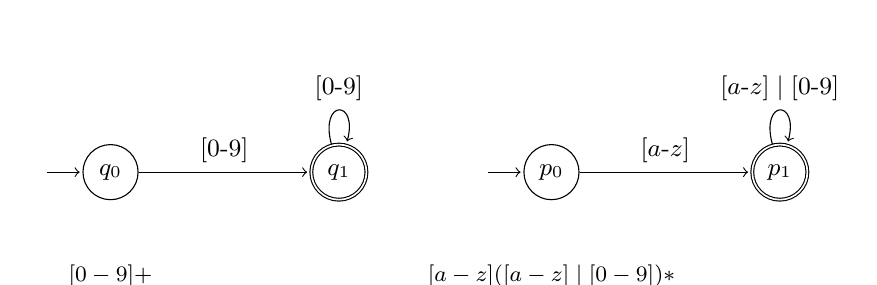
\begin{tikzpicture}[shorten >=1pt, node distance=2.9cm, on grid, auto,
      every state/.style={draw, minimum size=7mm, inner sep=1pt, font=\small},
      font=\small]
      \node[state, initial, initial text={}] (a0) {$q_0$};
      \node[state, accepting, right=of a0] (a1) {$q_1$};
      \path[->]
        (a0) edge node {$[0\text{-}9]$} (a1)
        (a1) edge [loop above] node {$[0\text{-}9]$} ();
      \node[below=1.05cm of a0, anchor=north, font=\footnotesize] {$[0-9]{+}$};

      \node[state, initial, initial text={}, right=5.6cm of a0] (b0) {$p_0$};
      \node[state, accepting, right=of b0] (b1) {$p_1$};
      \path[->]
        (b0) edge node {$[a\text{-}z]$} (b1)
        (b1) edge [loop above] node {$[a\text{-}z] \mid [0\text{-}9]$} ();
      \node[below=1.05cm of b0, anchor=north, font=\footnotesize]
        {$[a-z]([a-z] \mid [0-9]){*}$};
    \end{tikzpicture}
  \end{figure}
  Both have two useful états, and both spend one transition per character.
  Compare with running $\operatorname{match}$ over the syntax tree of the same
  expressions: the automate has already done that work, once, at construction
  time.
\end{example}

\subsubsection{Comparaison}
\begin{center}
  \begin{tabularx}{\textwidth}{@{}lX@{}}
    \toprule
    \textbf{Automates} & facile à manipuler pour l'ordinateur (union,
      intersection, test d'appartenance, etc.) ; difficile à comprendre pour un
      humain \\
    \midrule
    \textbf{Expressions régulières} & facile à comprendre pour un humain ; moins
      efficace algorithmiquement \\
    \bottomrule
  \end{tabularx}
\end{center}

\begin{conclusion}
  \emph{Ce que l'on veut : écrire des expressions régulières puis les compiler
  en automates !} One writes the notation that is readable and compiles it into
  the representation that is fast --- which is the same division of labour the
  whole module is about, one level down.
\end{conclusion}

\subsection{Analyse lexicale : le lexeur}
The \textit{lexeur} --- the analyseur lexical, the first pass of the
compilateur --- is the first real consumer of all of this.

\begin{definition}[Règles et actions]
  Une manière de faire des analyseurs lexicaux consiste à utiliser une liste
  d'expressions régulières $e_1 \ldots e_k$ et une liste d'actions
  $a_1 \ldots a_k$. Le lexeur va découper le mot en \textbf{lexèmes}
  $t_1 \ldots t_\ell$ et pour le lexème $t_j$ reconnu par $e_i$ il va faire
  l'action $a_i(t_j)$.
\end{definition}

\begin{figure}[h!]
  \centering
  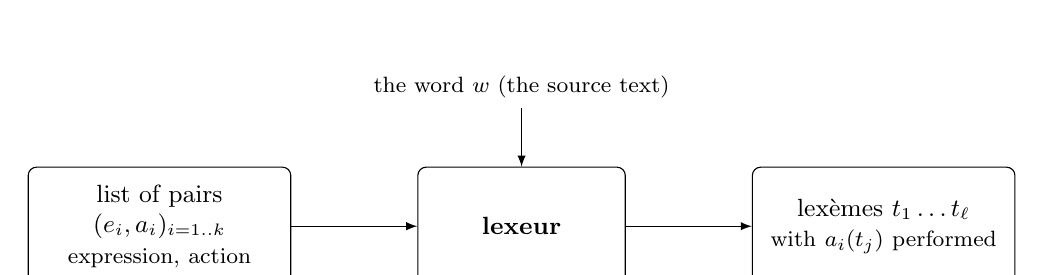
\begin{tikzpicture}[font=\small, node distance=0.6cm]
    \node[draw, rounded corners=3pt, minimum height=1.5cm, text width=3.1cm,
          align=center] (rules)
      {list of pairs\\ $(e_i, a_i)_{i=1..k}$\\ \footnotesize expression, action};
    \node[draw, rounded corners=3pt, minimum height=1.5cm, text width=2.4cm,
          align=center, right=1.6cm of rules] (lex) {\textbf{lexeur}};
    \node[draw, rounded corners=3pt, minimum height=1.5cm, text width=3.1cm,
          align=center, right=1.6cm of lex] (out)
      {lexèmes $t_1 \ldots t_\ell$\\ \footnotesize with $a_i(t_j)$ performed};
    \node[above=0.75cm of lex, font=\footnotesize] (src) {the word $w$ (the source text)};
    \path[->, >=latex]
      (rules) edge (lex)
      (lex) edge (out)
      (src) edge (lex);
  \end{tikzpicture}
\end{figure}

\subsubsection{Un exemple}
One text is run through one rule table, in order. Texte :
\begin{center}
  \texttt{let y\ \ \ = 42 in zzz+1\ \ \ \ 2+my\_var}
\end{center}
and the rules, \emph{in this order}, are

\begin{center}
  \begin{tabular}{@{}ll@{}}
    \toprule
    Expression & Action($x$) \\
    \midrule
    $[0-9]{+}$                        & Afficher \texttt{INT}($x$) \\
    \texttt{let}                      & Afficher \texttt{LET} \\
    \texttt{in}                       & Afficher \texttt{IN} \\
    \texttt{=}                        & Afficher \texttt{EQ} \\
    \texttt{'\ '}                     & Ignorer \\
    \texttt{+}                        & Afficher \texttt{PLUS} \\
    $[a-z]([a-z] \mid [0-9]){*}$      & Afficher \texttt{VAR}($x$) \\
    \bottomrule
  \end{tabular}
\end{center}

\noindent
Affichage :
\[
  \begin{array}{l}
    \texttt{LET},\;
    \texttt{VAR("y")},\;
    \texttt{EQ},\;
    \texttt{INT("42")},\;
    \texttt{IN},\;
    \texttt{VAR("zzz")},\;
    \texttt{PLUS}, \\[2pt]
    \texttt{INT("1")},\;
    \texttt{INT("2")},\;
    \texttt{PLUS},\;
    \texttt{VAR("my")},\;
    \textbf{ERREUR}.
  \end{array}
\]

\begin{figure}[h!]
  \centering
  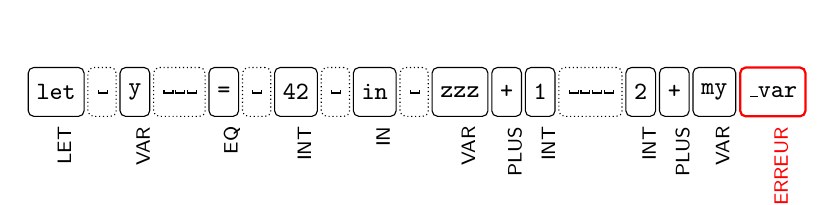
\begin{tikzpicture}[font=\ttfamily\small, node distance=0pt]
    \tikzset{
      tok/.style={draw, rounded corners=2pt, minimum height=0.62cm,
                  inner xsep=3pt, anchor=west},
      ign/.style={draw, densely dotted, rounded corners=2pt,
                  minimum height=0.62cm, inner xsep=3pt, anchor=west},
      lab/.style={font=\sffamily\scriptsize, rotate=90, anchor=east, yshift=-3pt},
    }
    \node[tok] (t1) at (0,0) {let};
    \node[ign, right=1pt of t1] (s1) {\textvisiblespace};
    \node[tok, right=1pt of s1] (t2) {y};
    \node[ign, right=1pt of t2] (s2) {\textvisiblespace\textvisiblespace\textvisiblespace};
    \node[tok, right=1pt of s2] (t3) {=};
    \node[ign, right=1pt of t3] (s3) {\textvisiblespace};
    \node[tok, right=1pt of s3] (t4) {42};
    \node[ign, right=1pt of t4] (s4) {\textvisiblespace};
    \node[tok, right=1pt of s4] (t5) {in};
    \node[ign, right=1pt of t5] (s5) {\textvisiblespace};
    \node[tok, right=1pt of s5] (t6) {zzz};
    \node[tok, right=1pt of t6] (t7) {+};
    \node[tok, right=1pt of t7] (t8) {1};
    \node[ign, right=1pt of t8] (s6) {\textvisiblespace\textvisiblespace\textvisiblespace\textvisiblespace};
    \node[tok, right=1pt of s6] (t9) {2};
    \node[tok, right=1pt of t9] (t10) {+};
    \node[tok, right=1pt of t10] (t11) {my};
    \node[tok, right=1pt of t11, draw=red, thick] (t12) {\_var};

    \node[lab] at (t1.south) {LET};
    \node[lab] at (t2.south) {VAR};
    \node[lab] at (t3.south) {EQ};
    \node[lab] at (t4.south) {INT};
    \node[lab] at (t5.south) {IN};
    \node[lab] at (t6.south) {VAR};
    \node[lab] at (t7.south) {PLUS};
    \node[lab] at (t8.south) {INT};
    \node[lab] at (t9.south) {INT};
    \node[lab] at (t10.south) {PLUS};
    \node[lab] at (t11.south) {VAR};
    \node[lab, text=red] at (t12.south) {ERREUR};
  \end{tikzpicture}
\end{figure}

Dotted boxes are the matches whose action is \emph{Ignorer}; they consume input
and emit nothing. The run stops at the underscore: no rule of the table matches
a prefix beginning with \verb|_|, so \texttt{my\_var} comes out as
\texttt{VAR("my")} followed by an error rather than as one identifier.

\subsubsection{L'algorithme, formellement}
\begin{definition}[La boucle du lexeur]
  Formellement, l'analyseur procède sur le mot $w = w_1 \ldots w_n$ de la façon
  suivante :
  \begin{itemize}
    \item s'il a fini de lire le mot ($n = 0$) il s'arrête ;
    \item sinon il regarde le \textbf{plus grand préfixe} $w_1 \ldots w_k$ du
      mot qui est reconnu par une des expressions $e_i$ ;
    \item si aucune expression ne reconnaît de préfixe, on déclenche une
      erreur ;
    \item parmi les expressions $e_i$ qui reconnaissent le préfixe
      $w_1 \ldots w_k$, il choisit celle avec le $i$ le \textbf{plus petit} ;
    \item il effectue $a_i(w_1 \ldots w_k)$ ;
    \item et continue sur le mot $w_{k+1} \ldots w_n$.
  \end{itemize}
\end{definition}

Two tie-breaks, applied in this order and only in this order. First the length:
the longest prefix matched by \emph{any} rule wins, whichever rule that is ---
le \textbf{plus grand préfixe} (\textit{maximal munch}). Only then, among the
rules that match that same longest prefix, the earliest in the list wins ---
la \textbf{priorité de la règle} (\textit{rule priority}). Everything a lexeur
specification does is arranged by these two.

\begin{example}[Priorité de la règle : why \texttt{let} is not a variable]
  At the start of the text, the prefix \texttt{let} is matched by rule $2$
  (\texttt{let}) and by rule $7$ ($[a-z]([a-z] \mid [0-9]){*}$), both of length
  $3$, and no rule matches anything longer --- the next character is a space.
  Length does not separate them; the priorité de la règle does, and rule $2$
  wins, so the lexème is \texttt{LET} and not \texttt{VAR("let")}. A keyword is
  simply a rule placed above the identifier rule.
\end{example}

\begin{example}[Plus grand préfixe : why \texttt{lettre} is not a keyword]
  Reverse the situation and feed the lexeur the text \texttt{lettre}. Rule $2$
  matches the prefix \texttt{let}, of length $3$; rule $7$ matches
  \texttt{lettre}, of length $6$. The first tie-break is the length, and $6 > 3$,
  so the priorité de la règle is never consulted: the lexème is
  \texttt{VAR("lettre")}. This is the whole reason the length test comes first
  --- with the priorité de la règle first, no identifier could ever begin with a
  keyword.
\end{example}

\begin{figure}[h!]
  \centering
  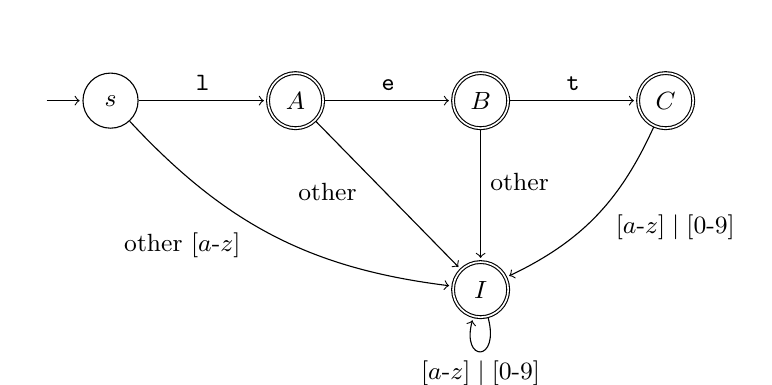
\begin{tikzpicture}[shorten >=1pt, node distance=2.35cm, on grid, auto,
    every state/.style={draw, minimum size=7mm, inner sep=1pt, font=\small},
    font=\small]
    \node[state, initial, initial text={}] (s) {$s$};
    \node[state, accepting, right=of s] (A) {$A$};
    \node[state, accepting, right=of A] (B) {$B$};
    \node[state, accepting, right=of B] (C) {$C$};
    \node[state, accepting, below=2.4cm of B] (I) {$I$};
    \path[->]
      (s) edge node {$\mathtt{l}$} (A)
      (A) edge node {$\mathtt{e}$} (B)
      (B) edge node {$\mathtt{t}$} (C)
      (s) edge [bend right=20] node[swap, pos=0.42] {other $[a\text{-}z]$} (I)
      (A) edge node[swap, pos=0.35] {other} (I)
      (B) edge node[pos=0.4] {other} (I)
      (C) edge [bend left=20] node[pos=0.42] {$[a\text{-}z]\mid[0\text{-}9]$} (I)
      (I) edge [loop below] node {$[a\text{-}z]\mid[0\text{-}9]$} ();
  \end{tikzpicture}
\end{figure}

The picture is the two rules \texttt{let} and $[a-z]([a-z]\mid[0-9]){*}$ merged
into one automate, which is what a lexeur generator actually builds; the edges
marked ``other'' carry every letter or digit except the one that continues the
keyword. The états $A$, $B$, $I$ are final for the identifier rule only, so
reaching them means \texttt{VAR}; $C$ is final for both rules at once, and it is
there that the priorité de la règle decides in favour of \texttt{LET}. The
scanner does not test the rules one after another --- it runs this single
automate, remembers the last état final it passed and which rules were
satisfied there, and on getting stuck falls back to that position. That is the
plus grand préfixe and the priorité de la règle, compiled.

\begin{remark}
  The rule \texttt{'\ '} of the table is a single quoted space --- one character,
  not one or more. Since its action is \emph{Ignorer}, a run of several spaces
  simply goes round the loop several times, which is why the four-space run in
  \texttt{zzz+1\ \ \ \ 2} costs four iterations and produces nothing (and the
  three-space gap before the \texttt{=} costs three). The
  \texttt{ocamllex} version below writes \texttt{[' ' '\textbackslash t'
  '\textbackslash n']+} instead, folding the repetition into the expression and
  also accepting tabs and newlines.
\end{remark}

\begin{remark}
  The error case is the only place the lexeur can fail, and it fails on a
  \emph{character}, not on a structure: it reports that no rule can start here.
  Everything about how the lexèmes fit together --- that \texttt{let} must be
  followed by a variable, that \texttt{+} needs two operands --- is beyond the
  lexeur's reach and is the parser's problem.
\end{remark}

\subsubsection{ocamllex}
Rather than write the loop by hand, one declares the rule table in a
\texttt{.mll} file and lets a generator emit the automate and the scanner.

\begin{lstlisting}[language=Caml]
{ open Lexing }

rule token = parse
  | ['0'-'9']+ as s { `INT (int_of_string s) }
  | "let"     { `LET }
  | "in"      { `IN }
  | '+'       { `PLUS }
  | '='       { `EQ }
  | [' ' '\t' '\n']+ { token lexbuf }
  | ['a'-'z']['a'-'z''0'-'9']* as id { `VAR id }
  | eof       { `EOF }
\end{lstlisting}

À mettre dans \texttt{lexer.mll} puis compiler avec \texttt{ocamllex lexer.mll}
--- \emph{utile pour votre compilateur !}\\

The correspondence with the table of the worked example is exact: each
\texttt{|} line is a pair $(e_i, a_i)$, the expression on the left in the
concrete syntax of the tool, the action on the right as an OCaml expression
between braces. Three points are specific to the tool.

\begin{itemize}
  \item \verb|as s| binds the matched text --- what the definition calls
    $w_1 \ldots w_k$, the argument $x$ of the action --- to a variable, so
    \texttt{INT} and \texttt{VAR} can carry it. Rules whose action ignores the
    text, such as \texttt{"let"}, need no binding.
  \item The whitespace rule's action is \texttt{token lexbuf}: it calls the
    scanner again on the rest of the input and returns whatever that returns.
    A recursive call \emph{is} how one writes \emph{Ignorer} when every rule has
    to produce a lexème.
  \item \texttt{eof} is an extra pattern the tool provides for end of input,
    turning the loop's termination condition into an ordinary rule; here it
    yields \texttt{`EOF}, a lexème the parser can match on.
\end{itemize}

\begin{remark}
  The results are backtick-prefixed --- \texttt{`INT}, \texttt{`LET} --- so they
  are OCaml \emph{polymorphic variants}: they need no type declared in advance,
  which is convenient for a type of lexèmes that grows as the compilateur does.
  The order of the lines is still load-bearing: \texttt{"let"} sits above the
  identifier rule for exactly the reason of the priorité de la règle example
  above.
\end{remark}

\subsubsection{Pourquoi un lexeur ?}
\begin{conclusion}
  Tout ce que le lexeur fait peut souvent être fait dans la grammaire mais ça :
  \begin{itemize}
    \item permet de décomposer le problème ;
    \item permet d'utiliser des expressions régulières ;
    \item simplifie beaucoup l'écriture et la lecture des grammaires ;
    \item diminue la complexité des grammaires.
  \end{itemize}
\end{conclusion}

The first clause is the honest one: a grammaire non contextuelle can generate
identifiers and integer literals character by character, so the lexeur is not a
necessity. It is a separation of concerns that pays. A grammar written over
lexèmes rather than characters has no rules for whitespace anywhere, does not
have to encode the plus grand préfixe as grammar rules, and --- since the
langages réguliers are a strict subclass of the languages of grammaires non
contextuelles --- hands the cheap part of the work to the cheap machine.

\subsection{Écrire un lexeur}
\begin{problem}[Objectif]
  Vous devez écrire du code qui implémente un petit lexeur, c'est-à-dire qui :
  \begin{itemize}
    \item récupère une liste de paires (expression régulière, nom) ;
    \item une chaîne de caractères ;
    \item et renvoie le résultat de l'analyse lexicale.
  \end{itemize}
\end{problem}

\noindent
\emph{Travailler avec méthode} : vous pouvez écrire les fonctions dans l'ordre
en testant chacune ; pensez à l'algorithme et s'il est correct ; réfléchissez à
ce qui est nécessaire au niveau du code.

\subsubsection{L'interface du lexeur}
Two extension files, \texttt{parser.ml} and \texttt{parser.py} --- the
continuation \emph{pour aller plus loin}, described in the last remark of this
chapter --- are written against the finished lexeur, so they pin down its
interface exactly. The rule list is the table of the worked example reordered
and slightly widened --- a rule for \texttt{*} is added, \texttt{INT} moves
below \texttt{ID}, \texttt{ident} also accepts capitals and \texttt{space} also
accepts a tab --- with a name in place of an action:

\begin{lstlisting}[language=Python]
rules = [
    (let_tok, "LET"), (in_tok, "IN"), (ope, "EQ"), (opp, "PLUS"),
    (opf, "FOIS"), (ident, "ID"), (digits, "INT"),
    (space, "SPACE")    # as in the worked example
]
\end{lstlisting}

\noindent
and it is consumed by a single function:

\begin{lstlisting}[language=Python]
list_tokens = lexer(rules, input_string)
rev_list_of_tokens = [("EOF","")] + list(reversed(
    [e for e in list_tokens if e[0] != "SPACE"]))
\end{lstlisting}

\begin{lstlisting}[language=Caml]
let token = ref ((lexer rules input_string
                  |> List.filter (fun (x,_) -> x != `SPACE))
                 @ [(`EOF,"")])
\end{lstlisting}

So \texttt{lexer} takes the rule list and the input chaîne de caractères and
returns a \emph{list of pairs} (name, matched text), in order of appearance ---
the OCaml version using polymorphic variants \texttt{`LET}, \texttt{`ID} as
names where the Python version uses chaînes de caractères. Three consequences
for the implementation.

\begin{itemize}
  \item The action of a rule is not a callback: it is just the name attached to
    the lexème, and the appelant decides what to do. \emph{Ignorer} is therefore
    not implemented in the lexeur at all --- \texttt{SPACE} lexèmes are produced
    like any other and the appelant filters them out, which is exactly what both
    snippets do before the analyse syntaxique.
  \item The matched text must be returned alongside the name, since the parser
    needs \texttt{"42"} to build the integer and the identifier's spelling to
    look it up in its environment (\texttt{Hashtbl.create 17} in OCaml,
    \texttt{dict()} in Python).
  \item The position of a rule in \texttt{rules} is the index $i$ of its
    priorité de la règle, so the list must be traversed in order: \texttt{LET}
    and \texttt{IN} precede \texttt{ID}, and an implementation that returns the
    first rule matching
    \emph{any} prefix, instead of the first rule matching the \emph{longest}
    prefix, will lex \texttt{lettre} as \texttt{LET} followed by
    \texttt{ID("tre")}.
\end{itemize}

\begin{remark}
  The natural shape of the code follows the two definitions of this chapter, in
  order: a \texttt{match} over the expression tree in the sense of the
  recognition equations, returning the set of end positions from a given start;
  then the loop of the lexeur, which at each position asks every rule for its
  end positions, keeps the largest $k$ over all rules, breaks ties by the
  smallest $i$, emits the pair and restarts at $k$. The error case is the one
  where every rule returns an empty set.
\end{remark}

\begin{remark}
  Une extension naturelle consiste à utiliser votre lexeur pour faire de
  l'analyse syntaxique. Vous pouvez utiliser les fichiers \texttt{parser.ml} ou
  \texttt{parser.py} à compléter pour avoir un parseur d'un langage contenant
  des entiers, des expressions \texttt{+}, \texttt{*} et des variables
  introduites par la syntaxe : \texttt{let \ldots = \ldots in \ldots}. The
  parser evaluates the expression to a number and fails if it is not parsable
  or uses an undefined variable. The skeleton they give --- a mutable list of
  lexèmes with \texttt{peek\_type} and \texttt{eat}, a hash table for the
  environment --- is a recursive-descent parser of exactly the kind the grammar
  chapter builds, which is why the grammar it is aimed at is the one that
  chapter asks to be made LL(1).
\end{remark}

\end{document}
